\documentclass[a4paper]{article}
\usepackage[a4paper,  fancysections,  titlepage]{pdfEPUSP}
\usepackage[brazilian]{babel}
\usepackage[hidelinks]{hyperref}
\usepackage[alf]{abntex2cite}
\usepackage{tcolorbox}
\usepackage[hypcap=false]{caption}
\usepackage{amsmath, amssymb}
\usepackage{placeins}

\usepackage{minted}
\setminted{
autogobble,
baselinestretch=0.9,
encoding=utf8,
fontsize=\footnotesize,
python3=true,
style=vs,
}

\author{
\begin{align*}
    &\text{Gabriel Pereira de Carvalho} \qquad &\text{NUSP: 11257668} \\
    &\text{Lucas Xavier de Morais} \qquad &\text{NUSP: 18066592} \\
    &\text{Joaquin Lorenzo Pereira Condori} \qquad &\text{NUSP: 11857963}
\end{align*}
}
\date{}
\title{PSI5723: Introdução ao Projeto de Sistemas VLSI em CMOS}
\subtitle{Lista de Exercícios 1}

\begin{document}

\maketitle

\tableofcontents
\newpage

\section{Cálculo dos parâmetros da porta NAND}

A porta NAND de duas entradas foi implementada em lógica CMOS estática no Cadence Virtuoso, conforme a Figura~\ref{fig:nand-esquematico}. Observa-se que na condição pedida para simulações com $A = B$, a porta se comporta como um inversor.

A rede de transistores PMOS é formada por dois dispositivos em paralelo entre a alimentação e a saída, enquanto a rede NMOS possui dois dispositivos em série entre a saída e o terra. Assim, a saída assume nível baixo apenas quando ambas as entradas estão em nível alto. Nas demais combinações, pelo menos um PMOS conduz e o caminho de descarga pelos NMOS é interrompido, estabelecendo nível alto na saída.

\begin{figure}[!htbp]
    \centering
    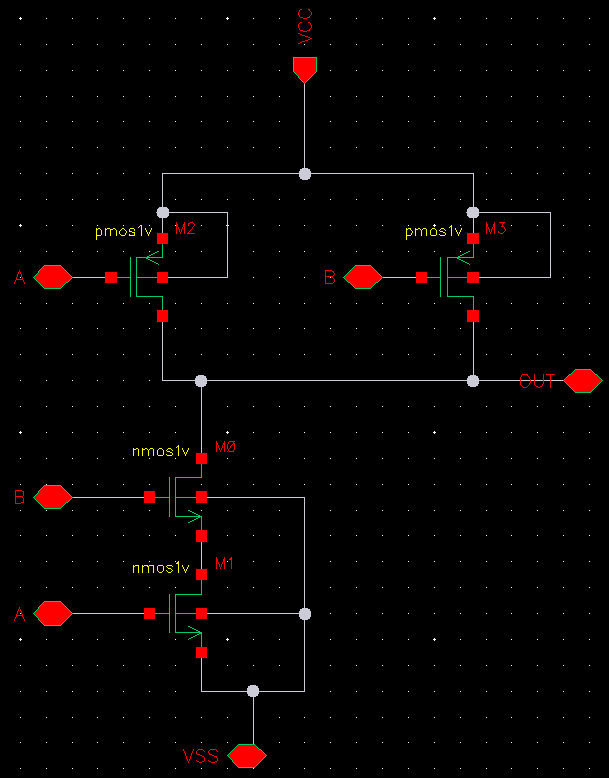
\includegraphics[width=0.95\linewidth]{imagens/NAND_schematic_2.png}
    \caption{Esquemático da porta NAND de duas entradas, com PMOS em paralelo e NMOS em série.}
    \label{fig:nand-esquematico}
\end{figure}

No esquemático, os quatro transistores apresentam comprimento de canal de $L = 130\,\mathrm{nm}$. Cada NMOS possui largura de $W_n = 1\,\mu\mathrm{m}$, enquanto a largura dos PMOS é parametrizada para permitir o ajuste do comportamento dinâmico da porta.

O circuito de teste é apresentado na Figura~\ref{fig:nand-testbench}. A alimentação é de $V_{DD} = 1{,}2\,\mathrm{V}$, com $V_{SS} = 0\,\mathrm{V}$, e a saída está conectada a uma capacitância de carga de $C_L = 10\,\mathrm{fF}$. Assim como especificado no enunciado, as entradas são excitadas por fontes pulsadas entre $0$ e $1{,}2\,\mathrm{V}$, com tempo de subida configurado em $60\,\mathrm{ps}$. %Essa carga deve ser considerada na interpretação dos tempos medidos, pois precisa ser carregada ou descarregada a cada transição da saída.

\begin{figure}[!htbp]
    \centering
    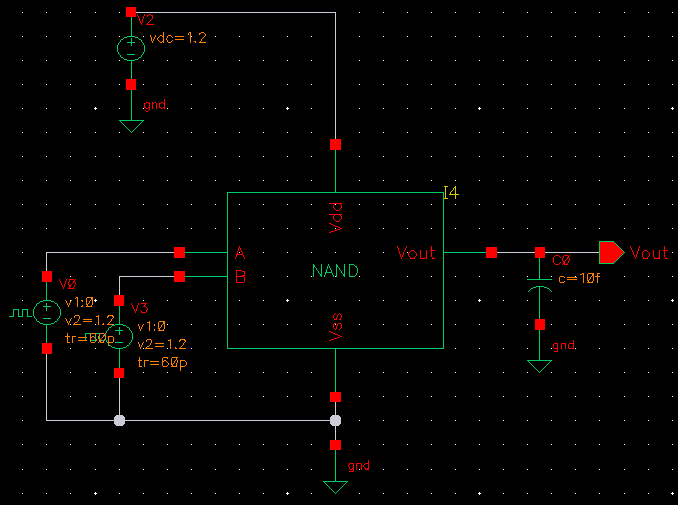
\includegraphics[width=0.70\linewidth]{imagens/NAND_tb_schematic.PNG}
    \caption{Circuito de teste da porta NAND, com alimentação de $1{,}2\,\mathrm{V}$, duas fontes de entrada e carga de $10\,\mathrm{fF}$.}
    \label{fig:nand-testbench}
\end{figure}

\subsection{Configuração da simulação no ADE}

A Figura~\ref{fig:nand-ade} mostra a configuração usada para análise transitória no Analog Design Environment (ADE). A simulação abrange o intervalo de $0$ a $5\,\mathrm{ns}$, à temperatura de $27\,^{\circ}\mathrm{C}$, com a variável \texttt{W\_pmos} representando a largura dos dispositivos PMOS. Para os plots foram selecionados o sinal de saída e das duas entradas, além de expressões para os tempos de carga e descarga, \texttt{tplh} e \texttt{tphl}, respectivamente.

\begin{figure}[!htbp]
    \centering
    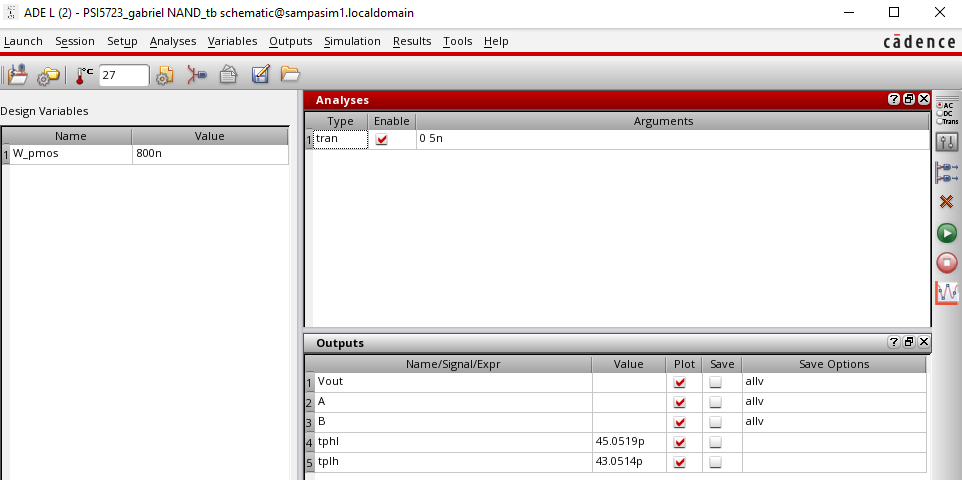
\includegraphics[width=0.90\linewidth]{imagens/NAND_tb_ADE.PNG}
    \caption{Configuração e resultados da simulação da NAND no ADE, com $W_p=800\,\mathrm{nm}$, temperatura de $27\,^{\circ}\mathrm{C}$ e análise transitória até $5\,\mathrm{ns}$.}
    \label{fig:nand-ade}
\end{figure}

\subsection{Varredura da largura dos transistores PMOS}

A variável \texttt{W\_pmos} foi utilizada na ferramenta Parametric Analysis, variada de $0{,}5$ a $2{,}0\,\mu\mathrm{m}$. A varredura permite comparar o atraso de propagação associado à subida da saída, $t_{pLH}$, com aquele associado à descida, $t_{pHL}$. Na Figura~\ref{fig:nand-atrasos-varredura}, observa-se que $t_{pLH}$ diminui com o aumento de \texttt{W\_pmos}, enquanto $t_{pHL}$ aumenta moderadamente.

A redução do atraso de subida é compatível com o aumento da capacidade de condução da rede PMOS. Já o aumento do atraso de descida é compatível com o acréscimo de capacitâncias associado ao aumento dos dispositivos, sem alteração da largura dos NMOS responsáveis pela descarga.

\begin{figure}[!htbp]
    \centering
    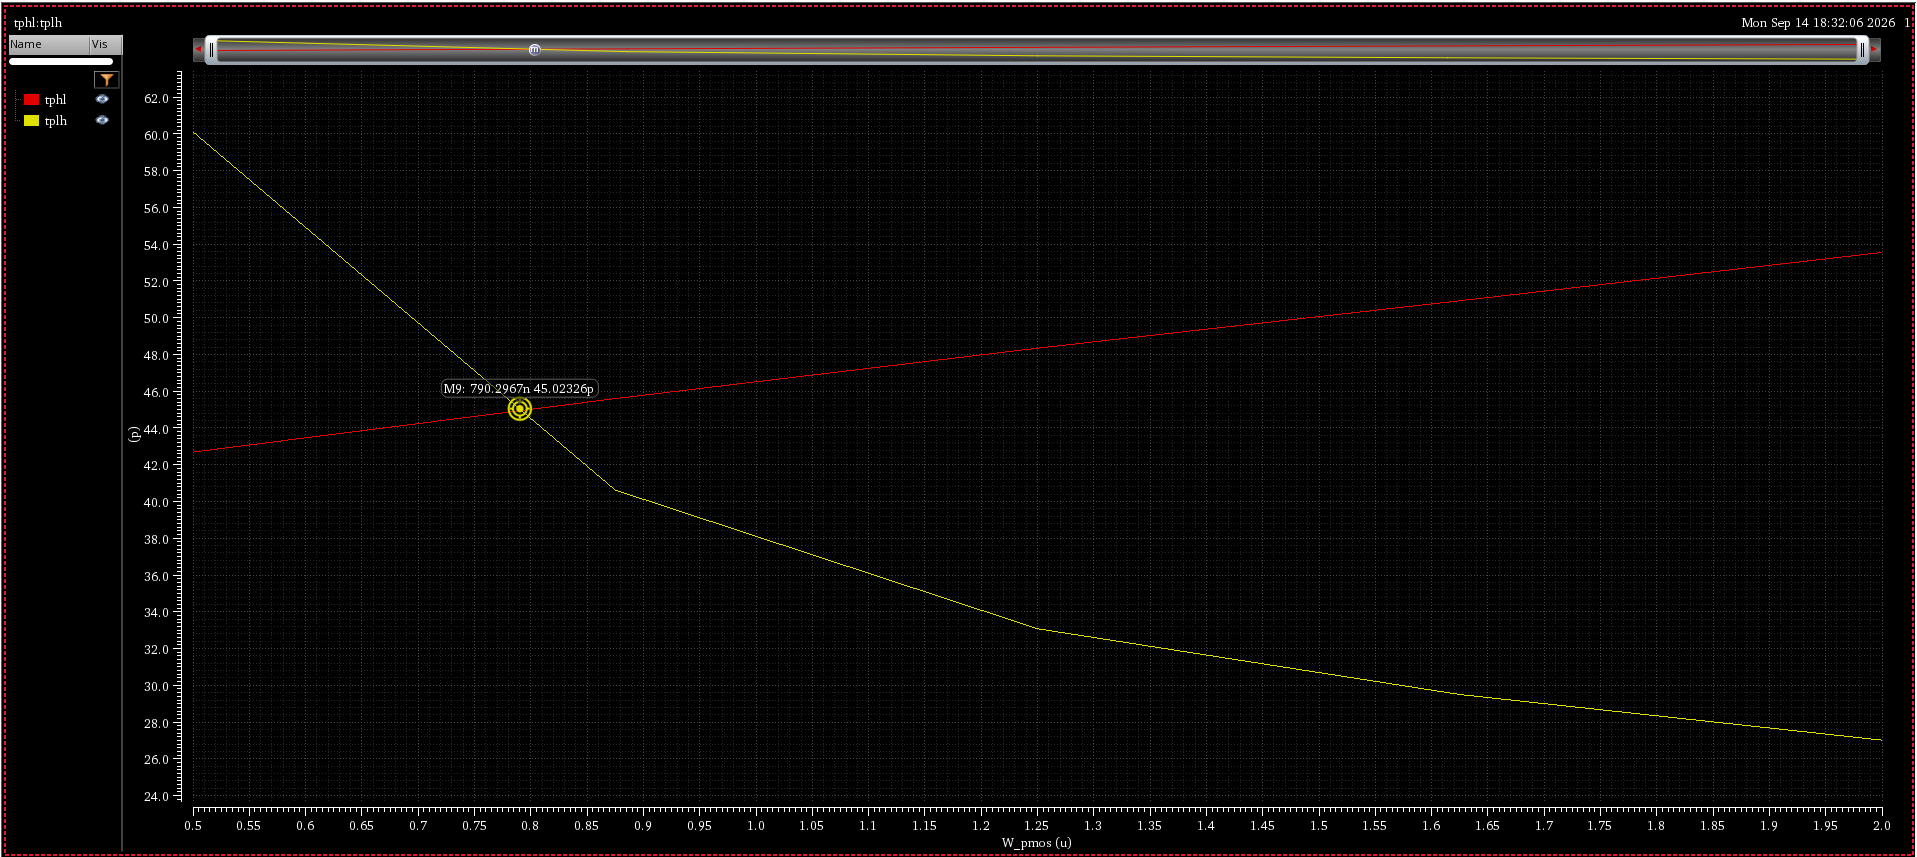
\includegraphics[width=\linewidth]{imagens/NAND_tb_tplh_tphl.PNG}
    \caption{Atrasos de propagação em função de \texttt{W\_pmos}: $t_{pLH}$ em amarelo e $t_{pHL}$ em vermelho. O marcador indica a região de equilíbrio entre os atrasos.}
    \label{fig:nand-atrasos-varredura}
\end{figure}

O marcador próximo à interseção das curvas indica uma largura de aproximadamente $790{,}3\,\mathrm{nm}$ e um atraso de $45{,}02\,\mathrm{ps}$. Portanto, a escolha de $W_p \approx 800\,\mathrm{nm}$ por transistor é uma referência para obter $t_{pLH} \approx t_{pHL}$ nas condições dessa varredura. Esse critério busca equilibrar os atrasos, não necessariamente minimizar cada um deles isoladamente.

\begin{tcolorbox}[
    title={Estimativa teórica para a largura dos PMOS da NAND},
    colback=bleu303pale,
    colframe=bleu303,
    fonttitle=\bfseries
]
Na condição simulada $A=B$, o caminho de carga é formado pelos dois PMOS em paralelo e na descarga os dois NMOS conduzem em série. Dessa forma, calculam-se os tempos de carga e descarga com $R_{p,\text{eq}} = \frac{R_p}{2}$ e $R_{n,\text{eq}} = 2R_n$ respectivamente

\begin{align}
    t_{pLH} &= 0,69 \left(\frac{R_p}{2}\right) C_L \\
    t_{pHL} &= 0,69 (2R_n) C_L
\end{align}

A igualdade $t_{pLH} = t_{pHL}$ ocorre quando
\begin{equation}
    4 \frac{R_n}{R_p} = 1 \iff 4 \left(\frac{W_p}{W_n}\right) \left(\frac{\mu_p}{\mu_n}\right) = 1 \iff W_p = \frac{1}{4}  \left(\frac{\mu_n}{\mu_p}\right) W_n
\end{equation}

Para $W_n=1\,\mu\mathrm{m}$ e adotando $\frac{\mu_n}{\mu_p} \approx 2$, a estimativa é $W_p \approx 500 \,\mathrm{nm}$. Assim, o valor experimental $W_p\approx 800 \,\mathrm{nm}$ está próximo do dimensionamento teórico da NAND.
\end{tcolorbox}

\subsection{Atrasos de propagação na análise transitória}

A Figura~\ref{fig:nand-marcadores} mostra a resposta transitória da saída e das duas entradas, identificadas nos gráficos como \texttt{/net5} e \texttt{/net6} com marcadores horizontais mostrando os pontos onde as curvas atingem $50\%$ da alimentação. No trecho apresentado, as entradas comutam simultaneamente: quando ambas sobem, a saída desce; quando ambas descem, a saída sobe. Esse comportamento é coerente com a função NAND para as combinações $A=B=0$ e $A=B=1$.

Conforme orientação do Professor Bruno, ignoramos os primeiros dois périodos na simulação, onde condições iniciais definidas no software poderiam impactar os valores medidos e utilizamos o trecho dos dois períodos seguintes para apresentar no relatório e realizar as medidas pedidas.

Os atrasos de propagação são medidos entre os cruzamentos da entrada e da saída por $50\%$ da alimentação, isto é, $0{,}6\,\mathrm{V}$:
\begin{align}
    t_{pLH} &= t_{\mathrm{out},\uparrow}(50\%) - t_{\mathrm{in},\downarrow}(50\%), \\
    t_{pHL} &= t_{\mathrm{out},\downarrow}(50\%) - t_{\mathrm{in},\uparrow}(50\%).
\end{align}

\begin{figure}[!htbp]
    \centering
    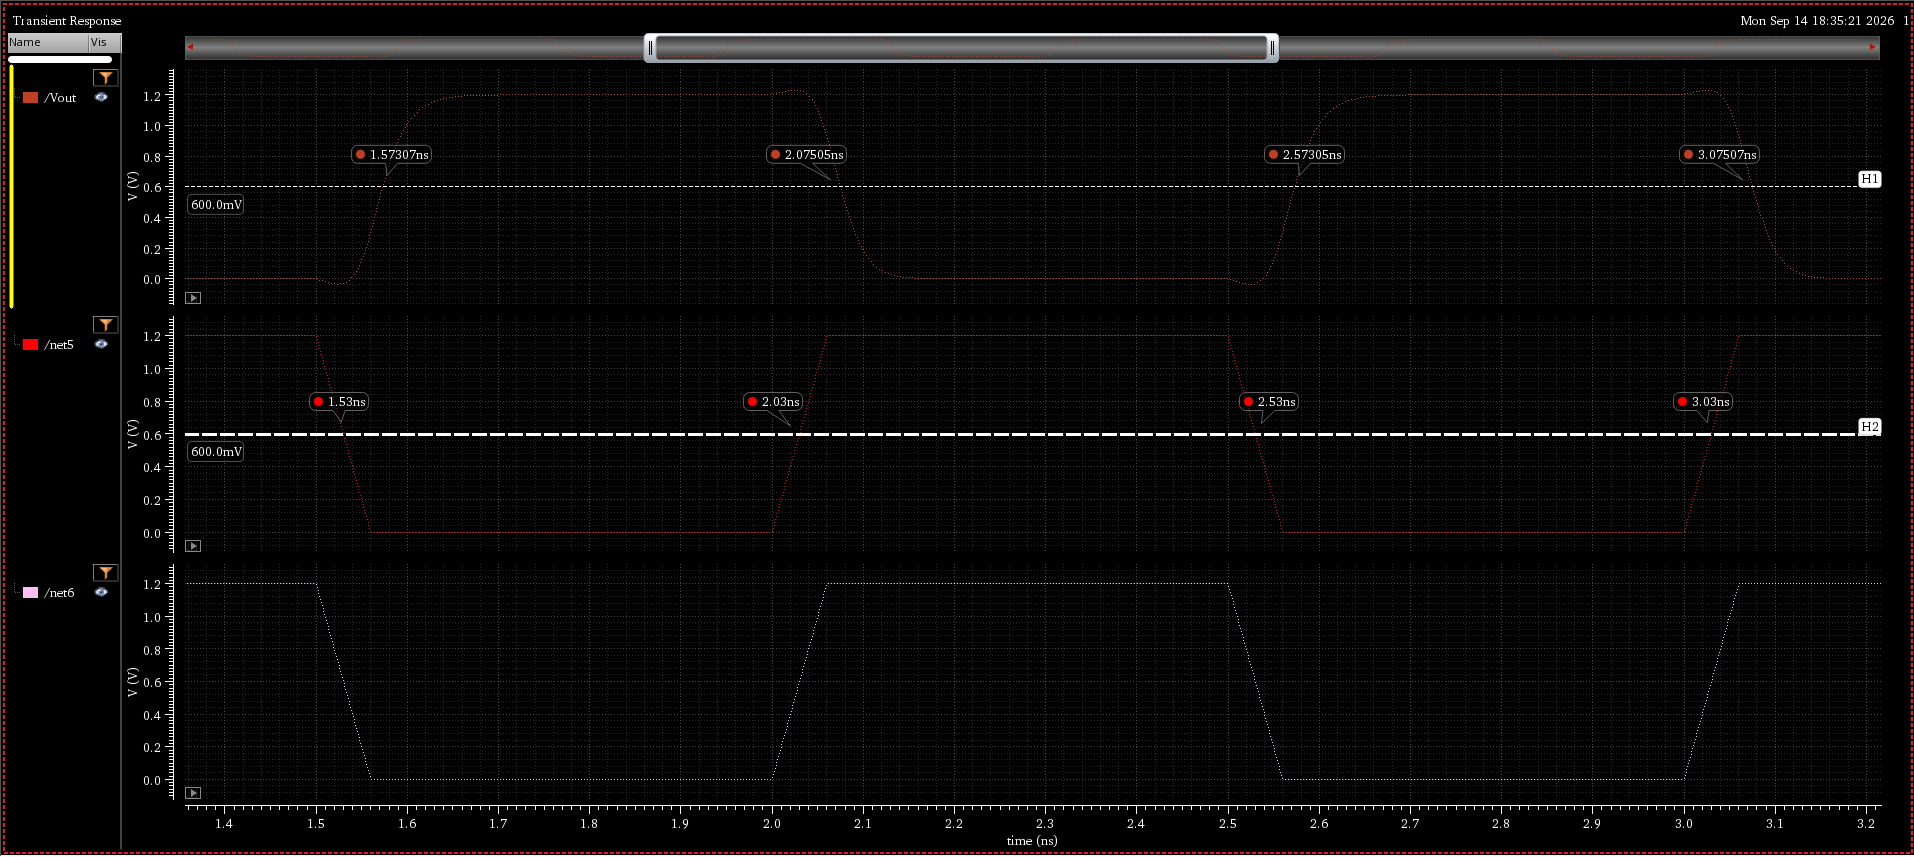
\includegraphics[width=\linewidth]{imagens/NAND_horizontal_markers.PNG}
    \caption{Medição dos atrasos de propagação por marcadores no nível de $600\,\mathrm{mV}$, correspondente a $50\%$ de $V_{DD}$.}
    \label{fig:nand-marcadores}
\end{figure}

Utilizando os marcadores do primeiro par de transições exibido na Figura~\ref{fig:nand-marcadores}, obtêm-se
\begin{align}
    t_{pLH} &= (1{,}57307 - 1{,}53000)\,\mathrm{ns}
             = 43{,}07\,\mathrm{ps}, \\
    t_{pHL} &= (2{,}07505 - 2{,}03000)\,\mathrm{ns}
             = 45{,}05\,\mathrm{ps}.
\end{align}
O atraso médio de propagação nesse par de transições é, portanto,
\begin{equation}
    t_p = \frac{t_{pLH}+t_{pHL}}{2}
        = 44{,}06\,\mathrm{ps}.
\end{equation}
No ciclo seguinte, os marcadores fornecem $t_{pLH} = 43{,}05\,\mathrm{ps}$ e $t_{pHL} = 45{,}07\,\mathrm{ps}$, valores próximos aos anteriores. Esses resultados são extraídos diretamente da resposta transitória e são consistentes com os valores das expressões inseridas no ADE para $W_p=800\,\mathrm{nm}$ (Figura~\ref{fig:nand-ade}). %As pequenas diferenças nas últimas casas decimais não alteram a conclusão de que os atrasos são próximos, mas devem ser distinguidos do valor na interseção da varredura.

\subsection{Tempos de subida e de descida}

Além dos atrasos de propagação, foram medidos os tempos de transição da própria saída, conforme a Figura~\ref{fig:nand-subida-descida} utilizando a ferramenta Direct Measurements do ADE. O critério selecionado na ferramenta utiliza os níveis de $10\%$ e $90\%$, aproximadamente $0{,}12\,\mathrm{V}$ e $1{,}08\,\mathrm{V}$. O tempo de subida, $t_r$, corresponde ao intervalo de $10\%$ a $90\%$, enquanto o tempo de descida, $t_f$, corresponde ao intervalo de $90\%$ a $10\%$.

\begin{figure}[!htbp]
    \centering
    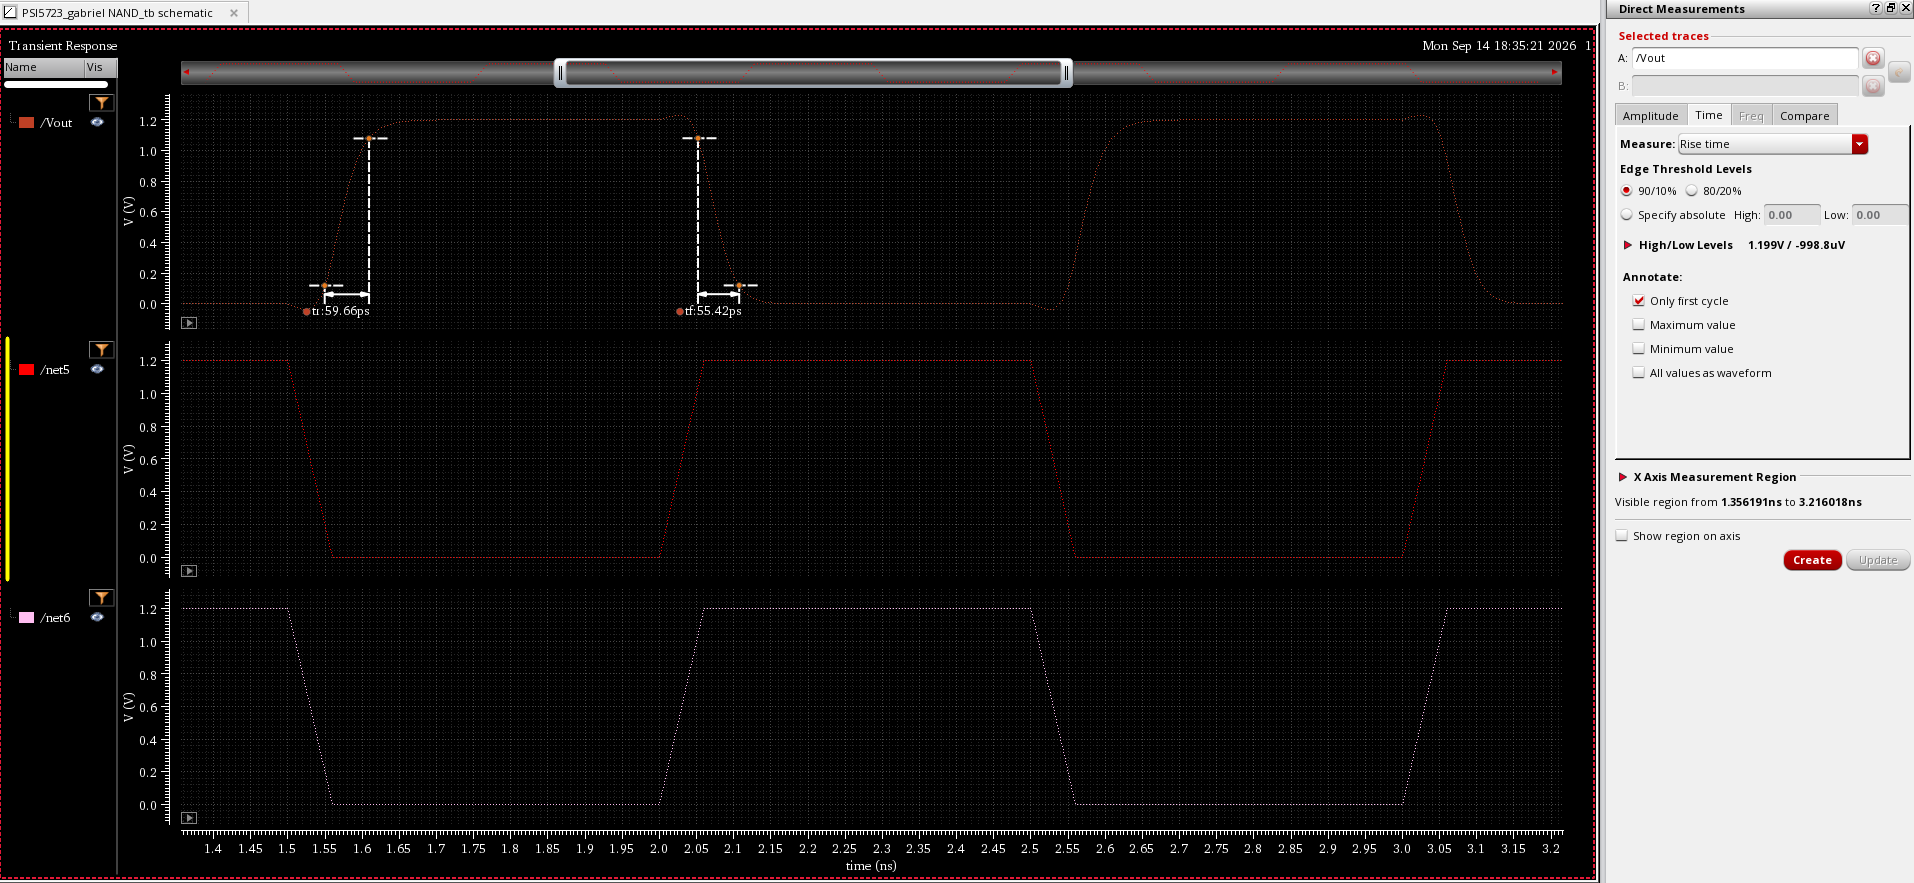
\includegraphics[width=\linewidth]{imagens/NAND_rise_fall_time.PNG}
    \caption{Medição dos tempos de subida e de descida da saída pelo critério de $10\%$--$90\%$, com $t_r = 59{,}66\,\mathrm{ps}$ e $t_f = 55{,}42\,\mathrm{ps}$.}
    \label{fig:nand-subida-descida}
\end{figure}

Os resultados de todas as medições que discutimos estão reunidos na Tabela~\ref{tab:nand-tempos}. Diferentemente dos atrasos de propagação, que relacionam uma transição de entrada à resposta da saída, $t_r$ e $t_f$ descrevem a duração das bordas da saída. Na condição apresentada, a subida é ligeiramente mais lenta que a descida, embora os atrasos de propagação sejam próximos.

\begin{table}[!htbp]
    \centering
    \caption{Resumo das medições transitórias da porta NAND em nível de esquemático, com $V_{DD}=1{,}2\,\mathrm{V}$ e $C_L=10\,\mathrm{fF}$. Os atrasos correspondem ao primeiro par de transições analisado.}
    \label{tab:nand-tempos}
    \begin{tabular}{lcc}
        \hline
        Grandeza & Critério de medição & Valor ($\mathrm{ps}$) \\
        \hline
        Atraso de subida, $t_{pLH}$ & Entrada--saída, $50\%$ & $43{,}07$ \\
        Atraso de descida, $t_{pHL}$ & Entrada--saída, $50\%$ & $45{,}05$ \\
        Atraso médio, $t_p$ & $(t_{pLH}+t_{pHL})/2$ & $44{,}06$ \\
        Tempo de subida, $t_r$ & Saída, $10\% \rightarrow 90\%$ & $59{,}66$ \\
        Tempo de descida, $t_f$ & Saída, $90\% \rightarrow 10\%$ & $55{,}42$ \\
        \hline
    \end{tabular}
\end{table}

% Essas medições caracterizam a porta no teste com comutação simultânea das entradas e carga de $10\,\mathrm{fF}$, sem resultados de extração de parasitas de layout apresentados nesta etapa. Elas constituem a referência de esquemático para a comparação posterior com o circuito extraído, mas não estabelecem, por si só, o pior caso de atraso entre todas as possíveis transições de entrada.

\subsection{Simulação nos corners SLOW e FAST}

A simulação da porta NAND nos corners SLOW e FAST, mantendo o mesmo valor de $W_p = 800 \,\mathrm{nm}$ e a capacitância de carga de $10\,\mathrm{fF}$ permite avaliar a influência das variações de processo, tensão de alimentação e temperatura. As Figuras~\ref{fig:nand-slow-config} e~\ref{fig:nand-fast-config} apresentam, respectivamente, as configurações das simulações SLOW e FAST. Os valores mostrados pelo ADE para os atrasos foram obtidos entre os cruzamentos das entradas e da saída por $50\%$ da tensão de alimentação. Dessa forma, os níveis de referência são $540\,\mathrm{mV}$ no corner SLOW e $660\,\mathrm{mV}$ no corner FAST.

\begin{figure}[!htbp]
    \centering
    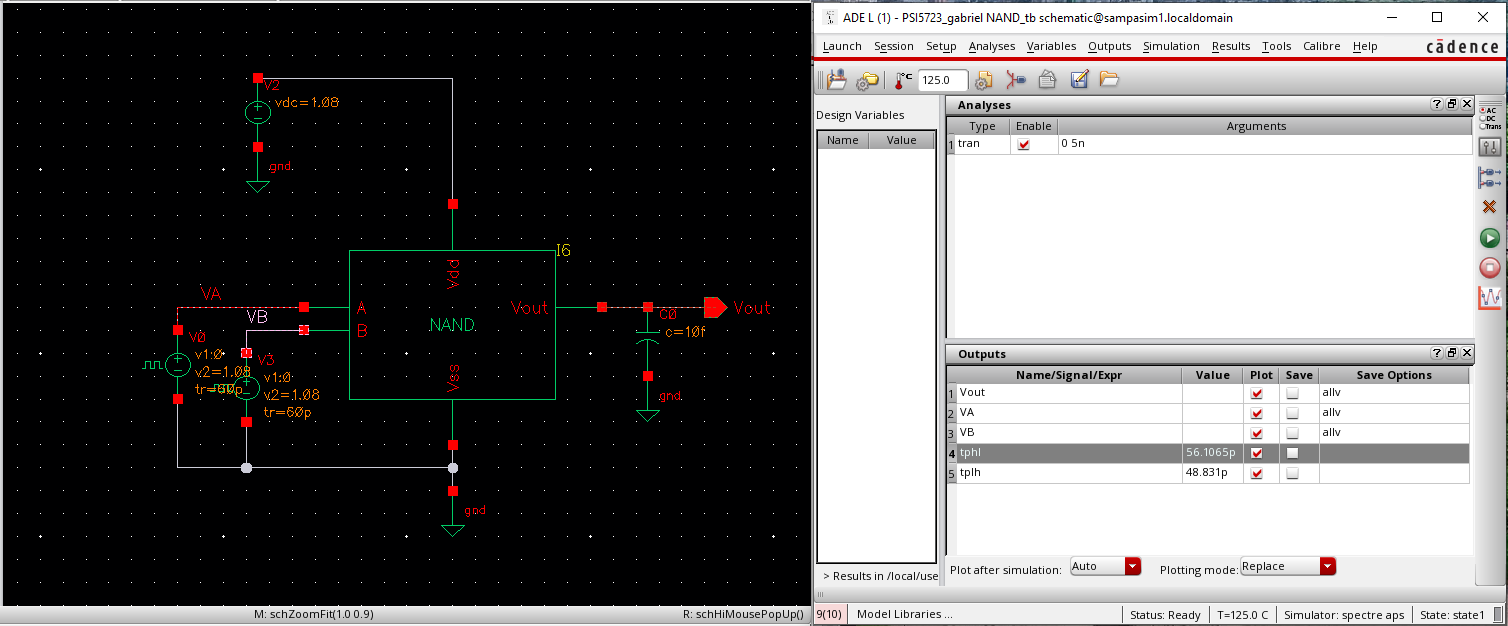
\includegraphics[width=\linewidth]{imagens/NAND_SLOW.PNG}
    \caption{Configuração da simulação da NAND no corner SLOW (WCS), com $V_{DD}=1{,}08\,\mathrm{V}$ e temperatura de $125\,^{\circ}\mathrm{C}$. O ADE fornece $t_{pHL}=56{,}1065\,\mathrm{ps}$ e $t_{pLH}=48{,}831\,\mathrm{ps}$.}
    \label{fig:nand-slow-config}
\end{figure}

\begin{figure}[!htbp]
    \centering
    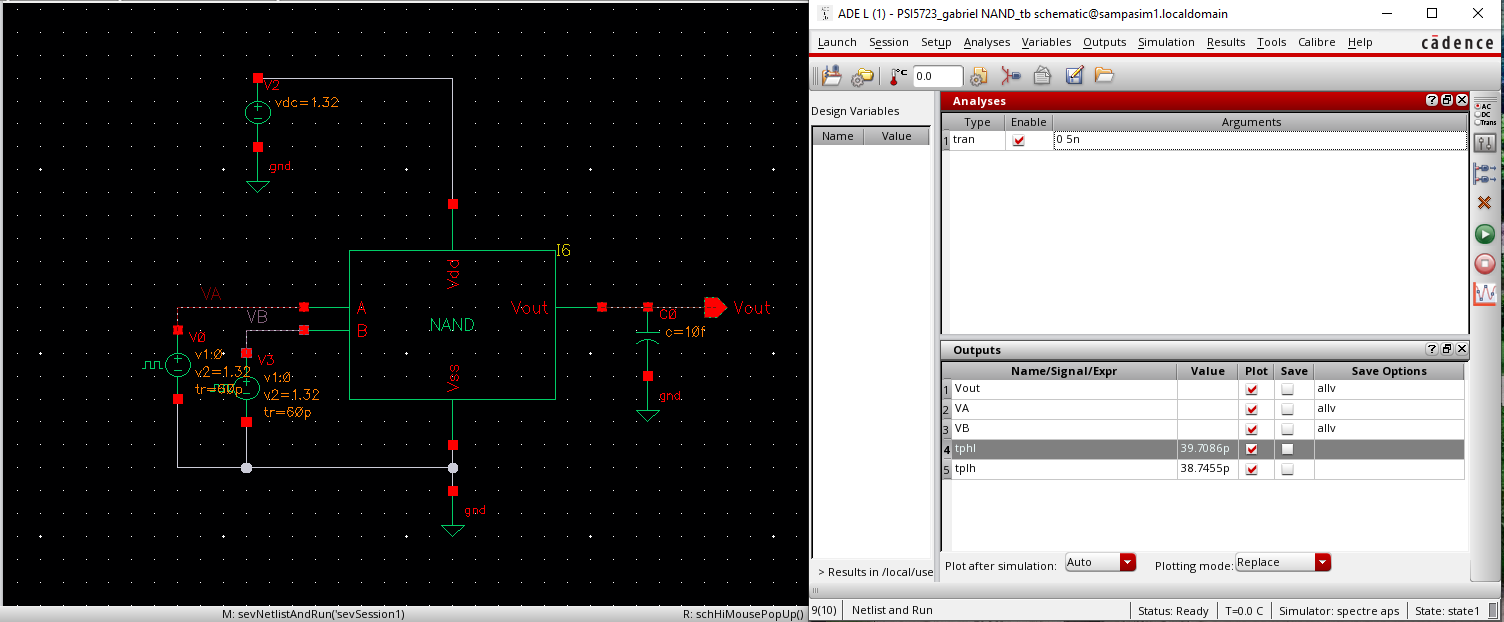
\includegraphics[width=\linewidth]{imagens/NAND_FAST.PNG}
    \caption{Configuração da simulação da NAND no corner FAST (WCP), com $V_{DD}=1{,}32\,\mathrm{V}$ e temperatura de $0\,^{\circ}\mathrm{C}$. O ADE fornece $t_{pHL}=39{,}7086\,\mathrm{ps}$ e $t_{pLH}=38{,}7455\,\mathrm{ps}$.}
    \label{fig:nand-fast-config}
\end{figure}

\subsubsection{Atrasos de propagação}

As medições por marcadores são apresentadas nas Figuras~\ref{fig:nand-slow-atrasos} e~\ref{fig:nand-fast-atrasos}. No corner SLOW, a transição de subida da entrada cruza $540\,\mathrm{mV}$ em $2{,}03000\,\mathrm{ns}$ e a saída cruza esse nível, durante a descida, em $2{,}08611\,\mathrm{ns}$. Para a transição oposta, os cruzamentos ocorrem em $2{,}53000\,\mathrm{ns}$ e $2{,}57883\,\mathrm{ns}$. Logo,
\begin{align}
    t_{pHL,\mathrm{SLOW}} &= (2{,}08611-2{,}03000)\,\mathrm{ns}
                            \approx 56{,}11\,\mathrm{ps}, \\
    t_{pLH,\mathrm{SLOW}} &= (2{,}57883-2{,}53000)\,\mathrm{ns}
                            = 48{,}83\,\mathrm{ps}.
\end{align}

\begin{figure}[!htbp]
    \centering
    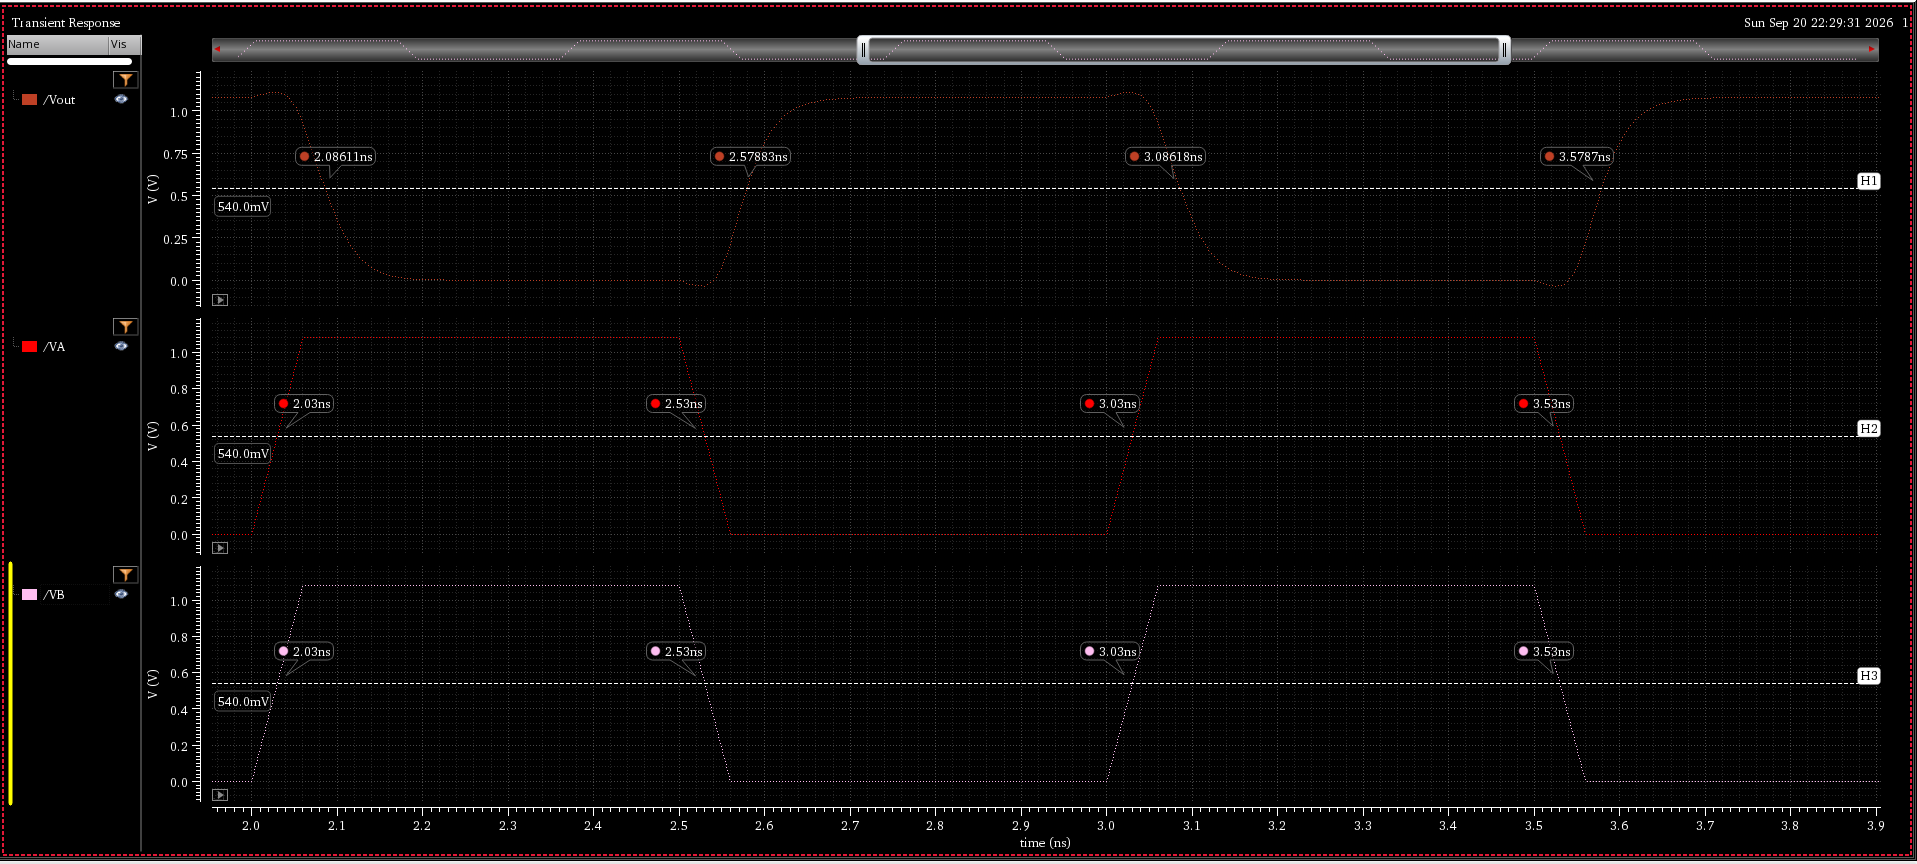
\includegraphics[width=\linewidth]{imagens/NAND_tphl_tplh_SLOW.PNG}
    \caption{Medição de $t_{pHL}$ e $t_{pLH}$ da NAND no corner SLOW, utilizando o nível de $540\,\mathrm{mV}$, correspondente a $50\%$ de $V_{DD}$.}
    \label{fig:nand-slow-atrasos}
\end{figure}

No corner FAST, os cruzamentos das entradas ocorrem em $2{,}03000\,\mathrm{ns}$ e $2{,}53000\,\mathrm{ns}$, enquanto os cruzamentos correspondentes da saída ocorrem em $2{,}069709\,\mathrm{ns}$ e $2{,}568745\,\mathrm{ns}$. Portanto,
\begin{align}
    t_{pHL,\mathrm{FAST}} &= (2{,}069709-2{,}030000)\,\mathrm{ns}
                            = 39{,}709\,\mathrm{ps}, \\
    t_{pLH,\mathrm{FAST}} &= (2{,}568745-2{,}530000)\,\mathrm{ns}
                            = 38{,}745\,\mathrm{ps}.
\end{align}

\begin{figure}[!htbp]
    \centering
    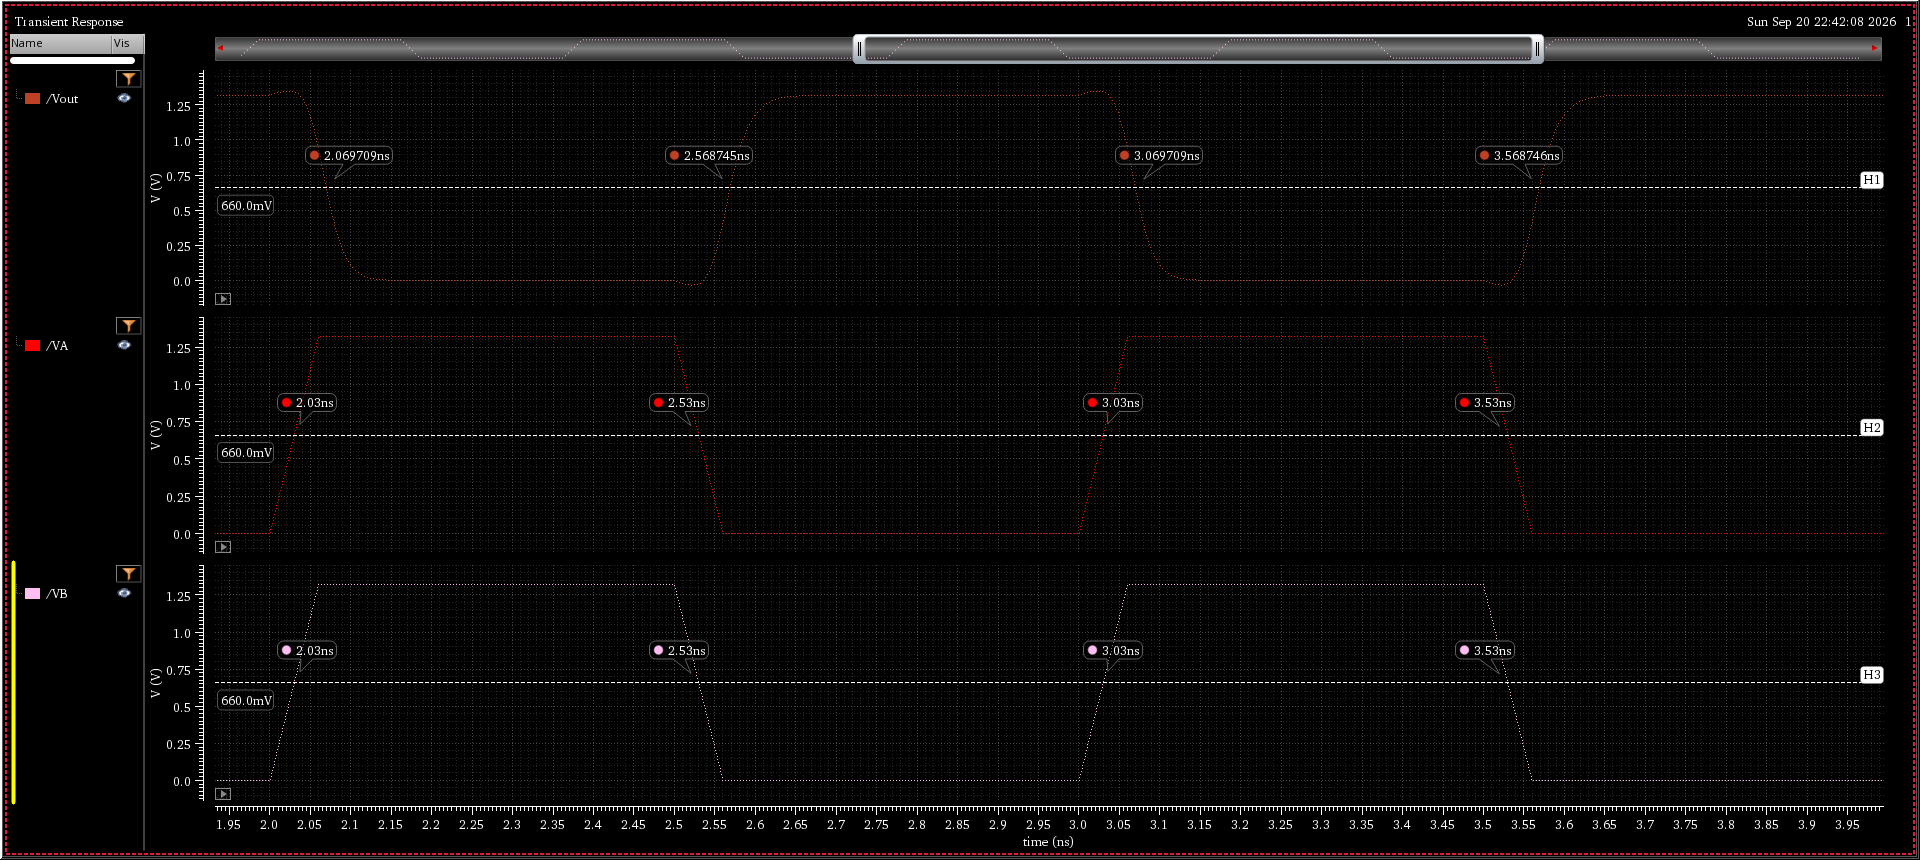
\includegraphics[width=\linewidth]{imagens/NAND_tphl_tplh_FAST.PNG}
    \caption{Medição de $t_{pHL}$ e $t_{pLH}$ da NAND no corner FAST, utilizando o nível de $660\,\mathrm{mV}$, correspondente a $50\%$ de $V_{DD}$.}
    \label{fig:nand-fast-atrasos}
\end{figure}

Os atrasos médios de propagação são $t_{p,\mathrm{SLOW}}=52{,}47\,\mathrm{ps}$ e $t_{p,\mathrm{FAST}}=39{,}23\,\mathrm{ps}$, calculados pela média entre $t_{pLH}$ e $t_{pHL}$ de cada corner.

\subsubsection{Tempos de subida e de descida}

Os tempos de transição da saída foram medidos na ferramenta Direct Measurements pelo critério de $10\%$--$90\%$ da excursão de tensão. As Figuras~\ref{fig:nand-slow-transicoes} e~\ref{fig:nand-fast-transicoes} mostram os resultados. Para o corner SLOW, foram obtidos $t_r=70{,}75\,\mathrm{ps}$ e $t_f=75{,}34\,\mathrm{ps}$. Para o corner FAST, foram obtidos $t_r=53{,}24\,\mathrm{ps}$ e $t_f=48{,}21\,\mathrm{ps}$.

\begin{figure}[!htbp]
    \centering
    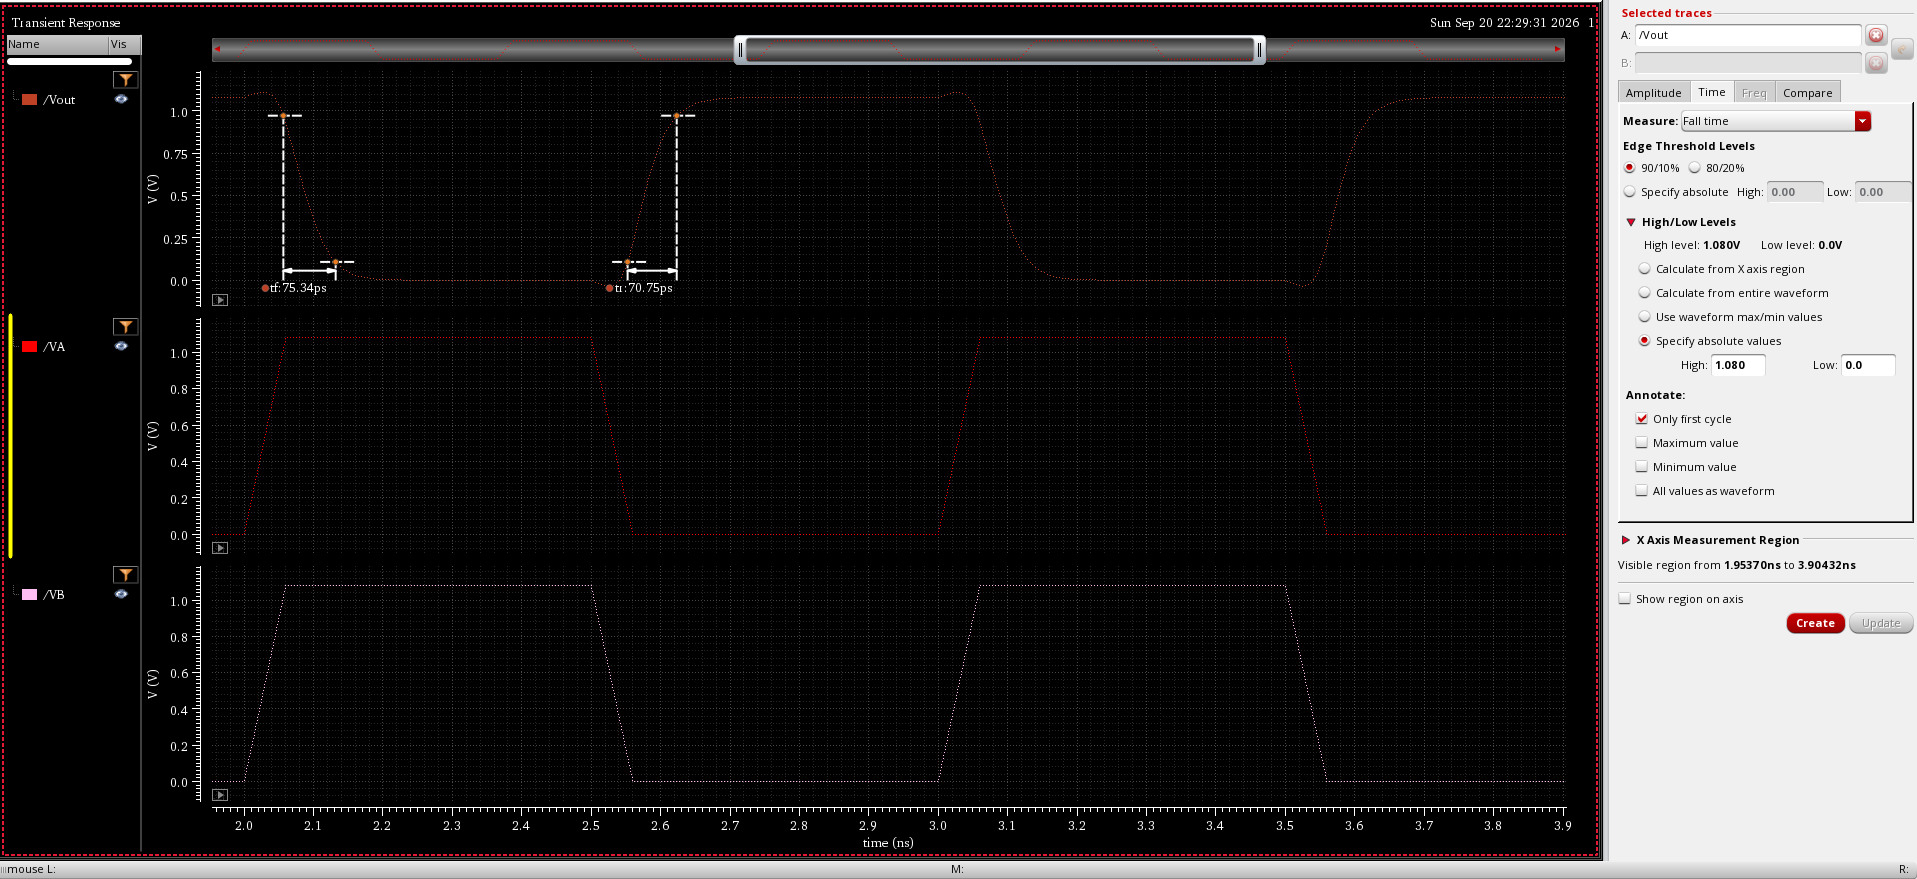
\includegraphics[width=\linewidth]{imagens/NAND_tf_tr_SLOW.PNG}
    \caption{Tempos de subida e de descida da NAND no corner SLOW, medidos pelo critério de $10\%$--$90\%$: $t_r=70{,}75\,\mathrm{ps}$ e $t_f=75{,}34\,\mathrm{ps}$.}
    \label{fig:nand-slow-transicoes}
\end{figure}

\begin{figure}[!htbp]
    \centering
    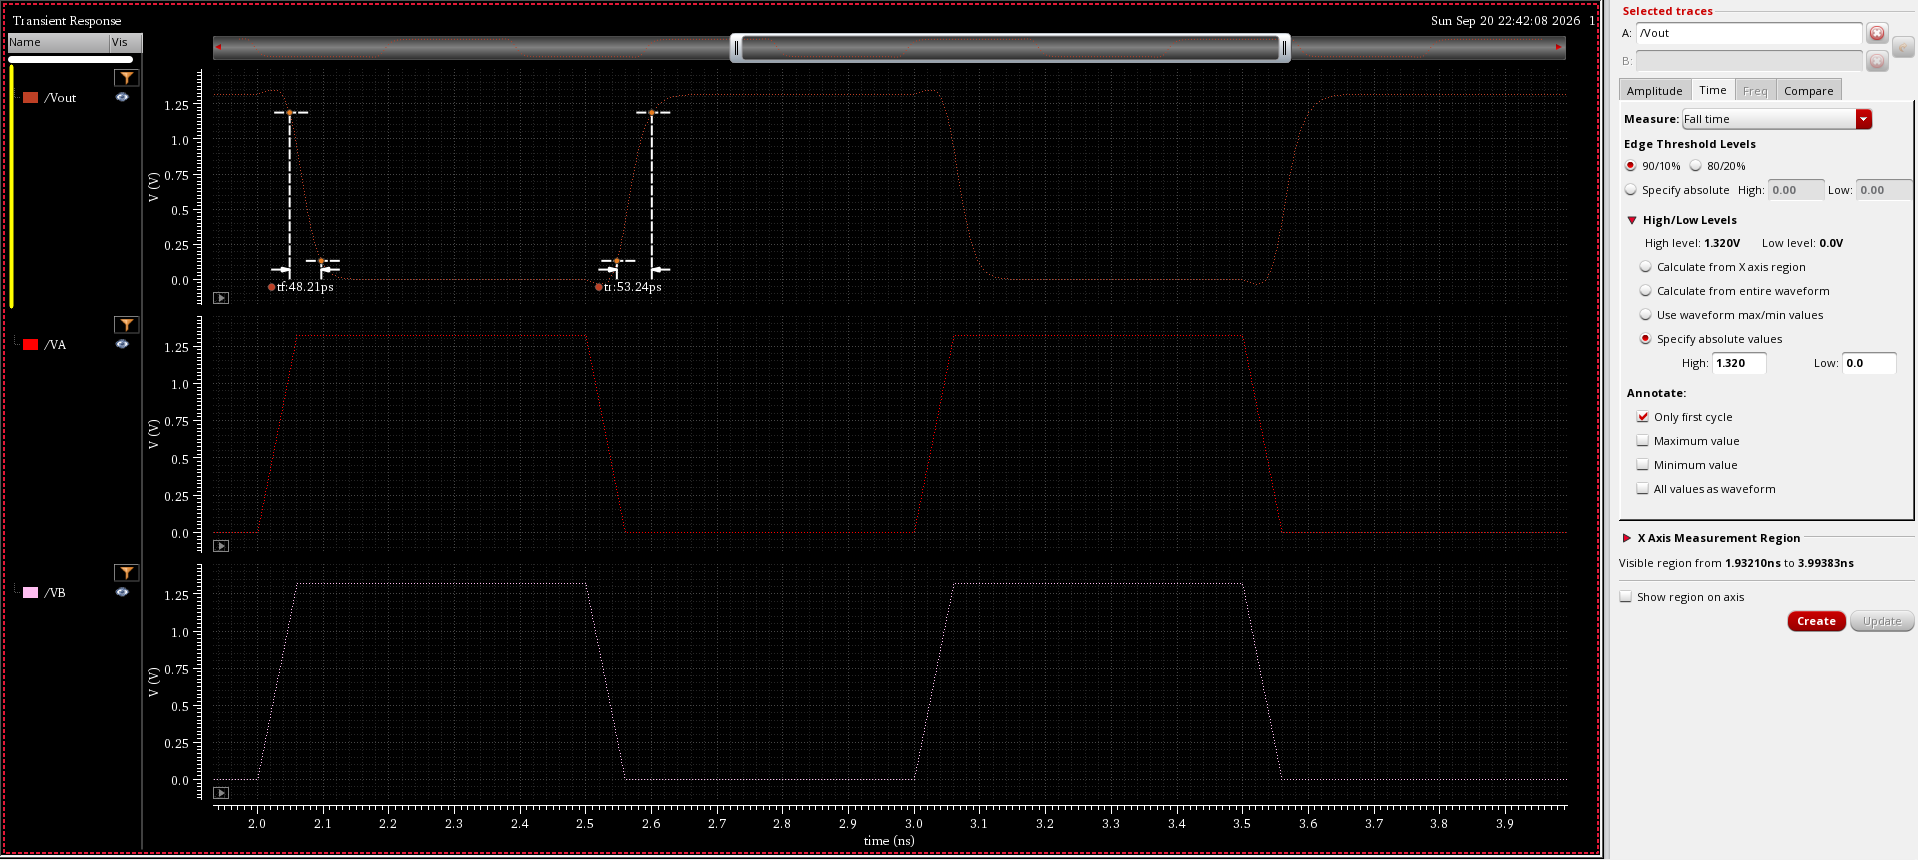
\includegraphics[width=\linewidth]{imagens/NAND_tf_tr_FAST.PNG}
    \caption{Tempos de subida e de descida da NAND no corner FAST, medidos pelo critério de $10\%$--$90\%$: $t_r=53{,}24\,\mathrm{ps}$ e $t_f=48{,}21\,\mathrm{ps}$.}
    \label{fig:nand-fast-transicoes}
\end{figure}

\FloatBarrier

\subsubsection{Comparação entre as condições de simulação}

A Tabela~\ref{tab:nand-corners} reúne todos os resultados obtidos nos corners típico, SLOW e FAST. Os valores típicos correspondem à simulação anterior com $V_{DD}=1{,}2\,\mathrm{V}$ e temperatura de $27\,^{\circ}\mathrm{C}$.

\begin{table}[!htbp]
    \centering
    \caption{Comparação dos tempos da porta NAND nas condições típica, SLOW e FAST.}
    \label{tab:nand-corners}
    \begin{tabular}{lcccccc}
        \hline
        Condição & $V_{DD}$ ($\mathrm{V}$) & $T$ ($^{\circ}\mathrm{C}$) & $t_{pLH}$ ($\mathrm{ps}$) & $t_{pHL}$ ($\mathrm{ps}$) & $t_r$ ($\mathrm{ps}$) & $t_f$ ($\mathrm{ps}$) \\
        \hline
        Típica & $1{,}20$ & $27$  & $43{,}07$ & $45{,}05$ & $59{,}66$ & $55{,}42$ \\
        SLOW   & $1{,}08$ & $125$ & $48{,}83$ & $56{,}11$ & $70{,}75$ & $75{,}34$ \\
        FAST   & $1{,}32$ & $0$   & $38{,}75$ & $39{,}71$ & $53{,}24$ & $48{,}21$ \\
        \hline
    \end{tabular}
\end{table}

Tomando a condição típica como referência, o corner SLOW aumenta $t_{pLH}$ em aproximadamente $13{,}4\%$ e $t_{pHL}$ em $24{,}5\%$. O atraso médio passa de $44{,}06\,\mathrm{ps}$ para $52{,}47\,\mathrm{ps}$, um aumento de cerca de $19{,}1\%$. Os tempos $t_r$ e $t_f$ aumentam, respectivamente, $18{,}6\%$ e $35{,}9\%$.

O maior impacto sobre $t_{pHL}$ e $t_f$ indica que, no corner SLOW, a descarga da saída pela associação em série dos NMOS é a transição mais penalizada. Esse comportamento é esperado no corner WCS: a menor alimentação reduz a sobre-excitação dos transistores, enquanto a temperatura elevada reduz a mobilidade dos portadores, diminuindo a corrente disponível para carregar e descarregar a capacitância de saída.

No corner FAST, $t_{pLH}$ diminui aproximadamente $10{,}0\%$ e $t_{pHL}$ diminui $11{,}9\%$ em relação à condição típica. O atraso médio é reduzido para $39{,}23\,\mathrm{ps}$, cerca de $11{,}0\%$ abaixo do valor típico. Da mesma forma, $t_r$ e $t_f$ diminuem $10{,}8\%$ e $13{,}0\%$, respectivamente.

A tensão de alimentação mais alta e a temperatura mais baixa aumentam a capacidade de condução dos transistores e tornam as transições mais rápidas. Essa melhora de velocidade ocorre na condição WCP, associada a maior consumo dinâmico devido ao aumento de $V_{DD}$, uma vez que a energia de comutação é aproximadamente proporcional a $C_LV_{DD}^{2}$.

Portanto, os resultados seguem a tendência física esperada: o corner SLOW estabelece o pior caso de velocidade, com todos os tempos superiores aos típicos, enquanto o corner FAST produz os menores atrasos e tempos de transição. Além disso, o equilíbrio entre $t_{pLH}$ e $t_{pHL}$ obtido no dimensionamento típico não é preservado exatamente nos corners extremos, pois as redes PMOS e NMOS não sofrem variações idênticas de mobilidade e corrente de condução.

\section{Desenho do layout da porta NAND}

O layout da porta NAND foi desenvolvido no Virtuoso a partir do dimensionamento obtido nas simulações de esquemático. A rede PMOS foi posicionada na parte superior, no interior do poço N, próxima à barra de $V_{DD}$, enquanto a rede NMOS foi posicionada na parte inferior, próxima à barra de $V_{SS}$. Essa organização segue o fluxo vertical convencional de uma célula CMOS e facilita a conexão dos corpos dos transistores às respectivas alimentações.

\subsection{Estratégia de desenho e roteamento}

A Figura~\ref{fig:nand-layout} apresenta a visão completa do layout. As barras de alimentação foram dispostas horizontalmente nas extremidades superior e inferior da célula. Para reduzir cruzamentos e facilitar a leitura das conexões, adotou-se como regra de roteamento o uso predominante de Metal~1 para os segmentos verticais e de Metal~2 para os segmentos horizontais. As mudanças de camada foram realizadas com vias nos pontos de conexão necessários. Essa separação de direções entre as camadas evita colisões entre as interconexões das entradas, da saída e das alimentações.

\begin{figure}[!htbp]
    \centering
    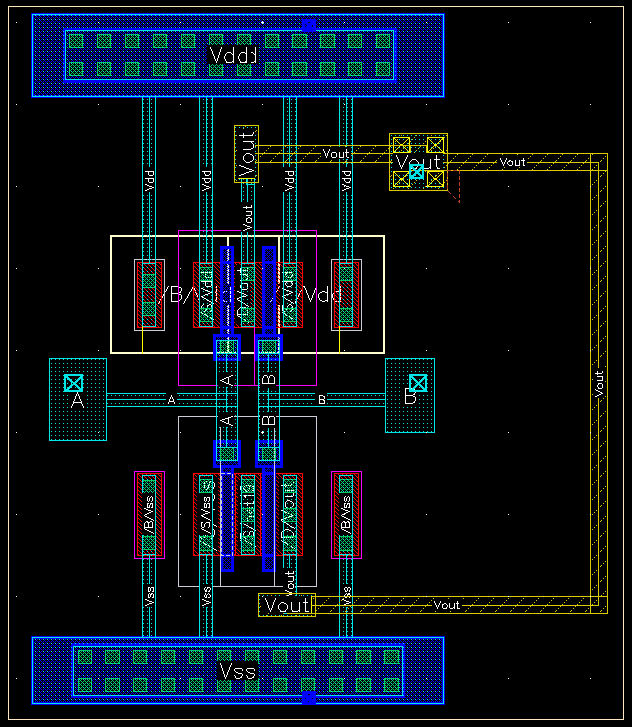
\includegraphics[width=0.72\linewidth]{imagens/NAND_layout.PNG}
    \caption{Layout completo da porta NAND, com a rede PMOS na região superior, a rede NMOS na região inferior e as interconexões em Metal~1 e Metal~2.}
    \label{fig:nand-layout}
\end{figure}

Os transistores de uma mesma rede foram aproximados para reduzir o comprimento das conexões entre terminais comuns e, consequentemente, a resistência e as capacitâncias parasitas associadas ao roteamento. Entretanto, não foi realizado o \textit{abutment} das regiões de difusão. A manutenção de regiões ativas separadas permitiu posicionar contatos individualmente e alinhar verticalmente a rede PMOS com a rede NMOS. Esse alinhamento simplificou o roteamento das entradas $A$ e $B$, cujas portas correspondentes puderam ser organizadas em colunas comuns às duas redes.

Na rede PMOS, os terminais conectados à alimentação foram conduzidos até a barra superior de $V_{DD}$, e os drenos associados à saída foram reunidos no nó $V_{out}$. Na rede NMOS, os dois dispositivos foram conectados em série, com o transistor inferior ligado à barra de $V_{SS}$ e o transistor superior ligado ao mesmo nó de saída. Contatos de poço e de substrato foram distribuídos próximos às respectivas redes para permitir a polarização dos terminais de \textit{body}. O nó $V_{out}$ foi conduzido até a lateral direita da célula, enquanto os pinos de entrada foram posicionados nas laterais, reduzindo a sobreposição com o roteamento interno.

\subsection{Definição dos pinos}

A Figura~\ref{fig:nand-pin-placement} mostra a configuração dos pinos no \textit{Pin Planner}, que permite a definição da camada onde cada pino foi desenhado no layout. %Os terminais $A$ e $B$ foram definidos como entradas, $V_{out}$ como saída e $V_{DD}$ e $V_{SS}$ como terminais de alimentação. %A definição e a conectividade dos pinos foram revisadas antes da verificação final, garantindo a correspondência dos cinco terminais entre o esquemático e o layout.

\begin{figure}[!htbp]
    \centering
    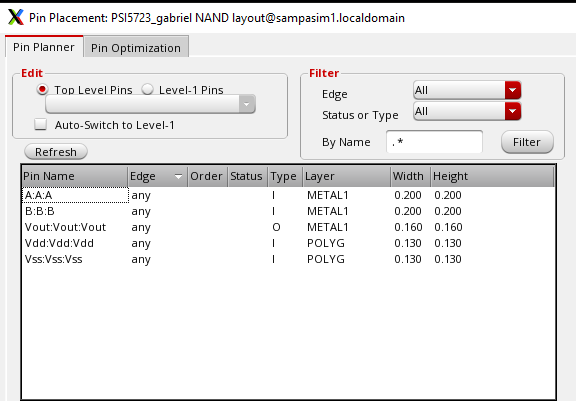
\includegraphics[width=0.78\linewidth]{imagens/NAND_pin_placement.PNG}
    \caption{Configuração dos pinos da célula NAND no \textit{Pin Planner}.}
    \label{fig:nand-pin-placement}
\end{figure}

\subsection{Verificação DRC}

A verificação das regras de projeto foi executada com o Calibre nmDRC. O resultado apresentado na Figura~\ref{fig:nand-drc} contém marcadores em 13 das 15 verificações listadas. A regra selecionada na captura, \texttt{OD.DN.3}, exige uma densidade mínima de $25\%$ da camada de difusão na área total do chip. Também são apresentados avisos equivalentes para diferentes camadas e áreas de impressão.

\begin{figure}[!htbp]
    \centering
    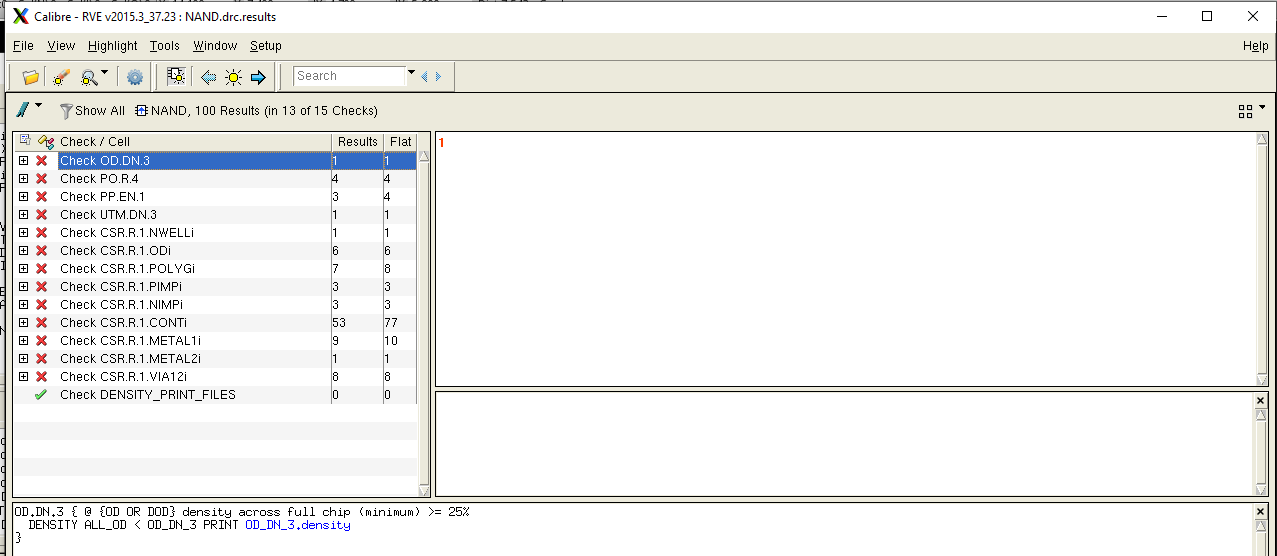
\includegraphics[width=\linewidth]{imagens/NAND_Callibre_nmDRC.PNG}
    \caption{Resultados do Calibre nmDRC para o layout da NAND. A regra selecionada corresponde a uma exigência global de densidade mínima da camada de difusão.}
    \label{fig:nand-drc}
\end{figure}

Como o arquivo contém apenas uma célula NAND isolada, sem o restante do chip, grande parte da área analisada permanece vazia. Por essa razão, os avisos globais de densidade e de área vazia foram desconsiderados nesta etapa. %Em um projeto destinado à fabricação, essa justificativa não seria suficiente: seria necessário inserir estruturas de preenchimento e executar novamente o DRC até obter um resultado limpo. Assim, o resultado atual deve ser interpretado como uma verificação preliminar da célula, e não como aprovação definitiva de DRC.

\subsection{Verificação LVS e extração de parasitas}

Após a revisão dos pinos e das conexões do layout, foi executada a verificação \textit{Layout Versus Schematic} no Calibre. A Figura~\ref{fig:nand-lvs} apresenta o resultado \textit{CORRECT}: layout e esquemático possuem cinco portas, seis redes e quatro transistores, sendo dois NMOS e dois PMOS. Assim, foi confirmada a equivalência elétrica entre as duas representações da porta NAND.

\begin{figure}[!htbp]
    \centering
    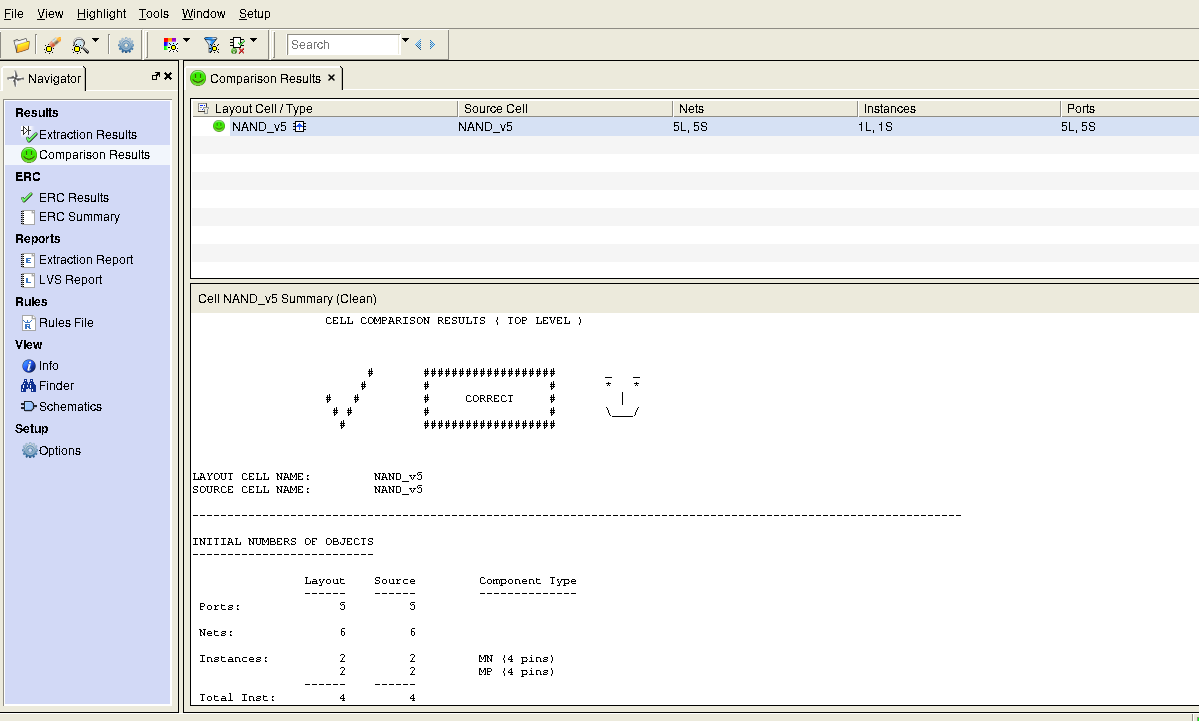
\includegraphics[width=0.95\linewidth]{imagens/LVS_update/NAND_LVS_validated.png}
    \caption{Resultado da verificação LVS da porta NAND no Calibre, com correspondência correta entre layout e esquemático.}
    \label{fig:nand-lvs}
\end{figure}

Com o LVS validado, utilizou-se o Calibre PEX para extrair as resistências e capacitâncias parasitas do layout. A Tabela~\ref{tab:nand-parasitas} apresenta o resumo da extração por rede. A coluna \texttt{R\_Count} indica a quantidade de elementos resistivos extraídos; $C_{\mathrm{tot}}$ representa a capacitância da rede para o substrato; $C_C$ corresponde à capacitância de acoplamento com outras redes; e a última coluna apresenta a soma dessas duas contribuições.

\begin{table}[!htbp]
    \centering
    \scriptsize
    \caption{Resumo dos parasitas extraídos pelo Calibre PEX para cada rede do layout da NAND.}
    \label{tab:nand-parasitas}
    \resizebox{\linewidth}{!}{%
    \begin{tabular}{llcccc}
        \hline
        Rede no layout & Rede no esquemático & \texttt{R\_Count} & $C_{\mathrm{tot}}$ ($\mathrm{F}$) & $C_C$ ($\mathrm{F}$) & $C_{\mathrm{tot}}+C_C$ ($\mathrm{F}$) \\
        \hline
        \texttt{A}    & \texttt{A}    & $8$  & $2{,}20492\times10^{-16}$ & $7{,}75235\times10^{-17}$ & $2{,}98015\times10^{-16}$ \\
        \texttt{B}    & \texttt{B}    & $8$  & $1{,}95120\times10^{-16}$ & $1{,}65963\times10^{-16}$ & $3{,}61083\times10^{-16}$ \\
        \texttt{VOUT} & \texttt{VOUT} & $22$ & $3{,}55737\times10^{-16}$ & $4{,}74046\times10^{-16}$ & $8{,}29783\times10^{-16}$ \\
        \texttt{VSS}  & \texttt{VSS}  & $15$ & $1{,}02883\times10^{-15}$ & $2{,}22095\times10^{-16}$ & $1{,}25092\times10^{-15}$ \\
        \texttt{VDD}  & \texttt{VDD}  & $21$ & $9{,}92209\times10^{-16}$ & $1{,}74824\times10^{-16}$ & $1{,}16703\times10^{-15}$ \\
        \texttt{6}    & \texttt{NET1} & $5$  & $8{,}83051\times10^{-17}$ & $2{,}11377\times10^{-16}$ & $2{,}99682\times10^{-16}$ \\
        \hline
    \end{tabular}%
    }
\end{table}

As maiores capacitâncias totais da NAND aparecem nas redes de alimentação: $1{,}25092\,\mathrm{fF}$ em $V_{SS}$ e $1{,}16703\,\mathrm{fF}$ em $V_{DD}$. A saída apresenta $0{,}829783\,\mathrm{fF}$, dos quais $0{,}474046\,\mathrm{fF}$ correspondem ao acoplamento com outras redes.

O circuito extraído foi então simulado nas condições típica, SLOW e FAST. Nas Figuras~\ref{fig:nand-pex-normal}--\ref{fig:nand-pex-fast}, os atrasos foram obtidos pela diferença entre os cruzamentos correspondentes da entrada e da saída. Os tempos de subida e de descida são as medições de $10\%$--$90\%$ indicadas pelos marcadores das próprias formas de onda.

\begin{figure}[!htbp]
    \centering
    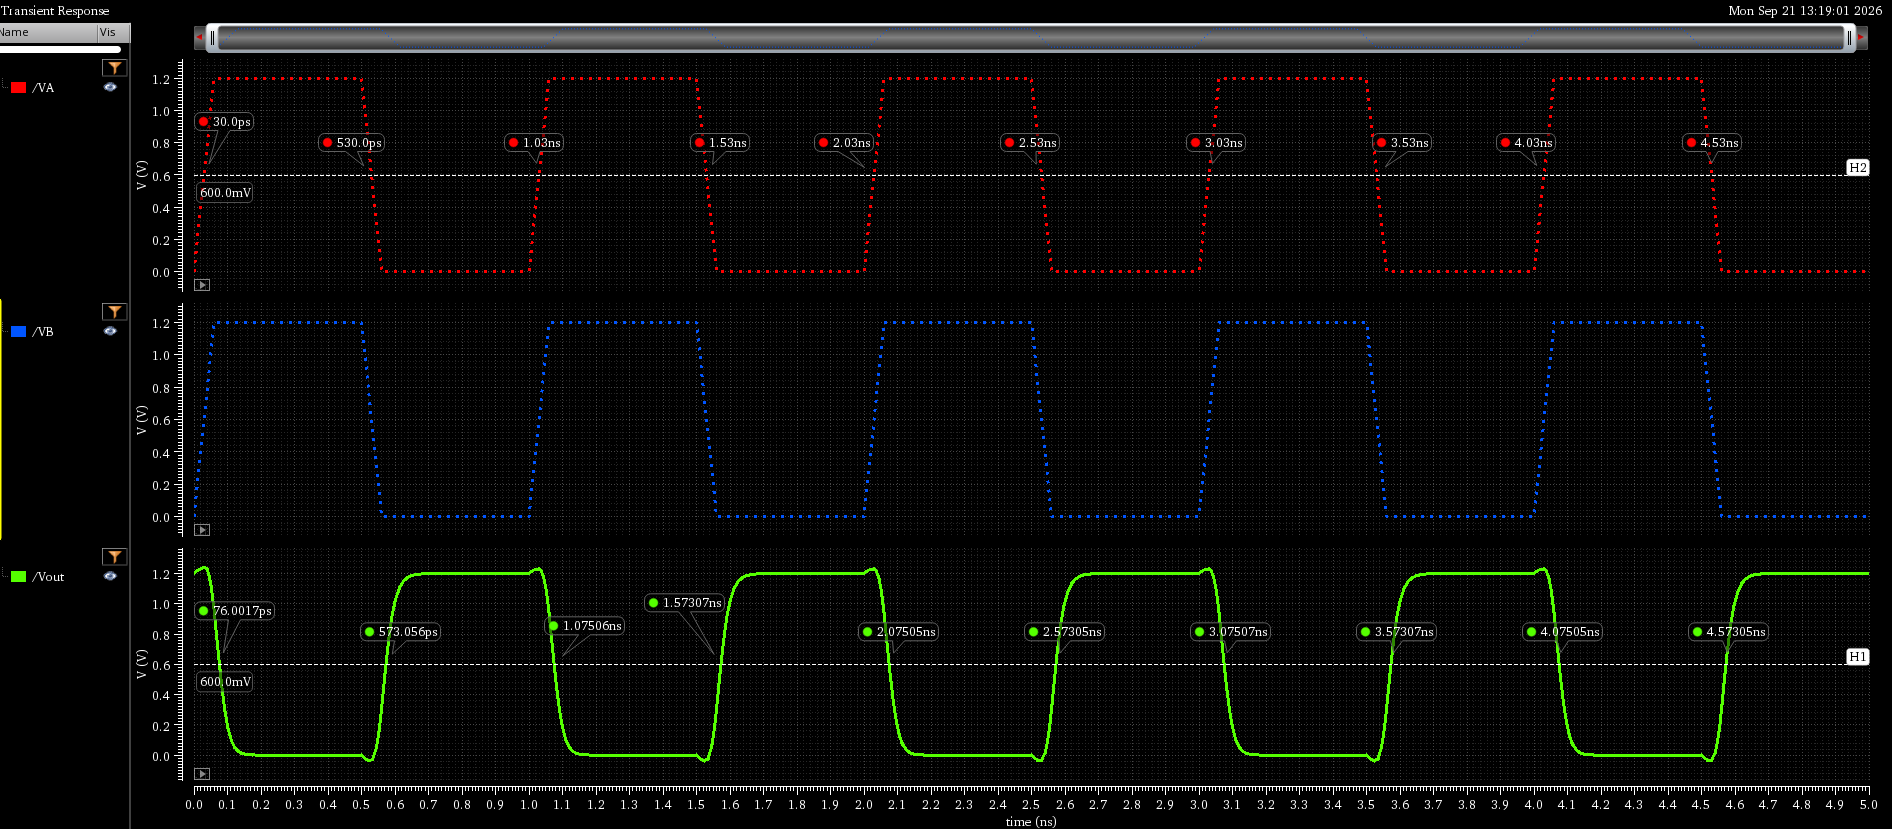
\includegraphics[width=\linewidth]{imagens/LVS_update/NAND_PEX_NORMAL_SIMULATION_2.png}
    \caption{Simulação PEX da NAND na condição típica para a medição dos atrasos de propagação: $t_{pLH}=43{,}07\,\mathrm{ps}$ e $t_{pHL}=45{,}06\,\mathrm{ps}$.}
    \label{fig:nand-pex-normal}
\end{figure}

\FloatBarrier

Utilizando os marcadores da Figura~\ref{fig:nand-pex-normal}, na condição típica, obtêm-se
\begin{align}
    t_{pHL} &= (1{,}07506-1{,}03000)\,\mathrm{ns}
             =45{,}06\,\mathrm{ps}, \\
    t_{pLH} &= (1{,}57307-1{,}53000)\,\mathrm{ns}
             =43{,}07\,\mathrm{ps}, \\
    t_p &= \frac{t_{pLH}+t_{pHL}}{2}
          =44{,}07\,\mathrm{ps}.
\end{align}
Os tempos de transição foram extraídos separadamente da Figura~\ref{fig:nand-pex-normal-transicoes}, utilizando os níveis de $10\%$ e $90\%$ de $V_{DD}$.
\begin{figure}[!htbp]
    \centering
    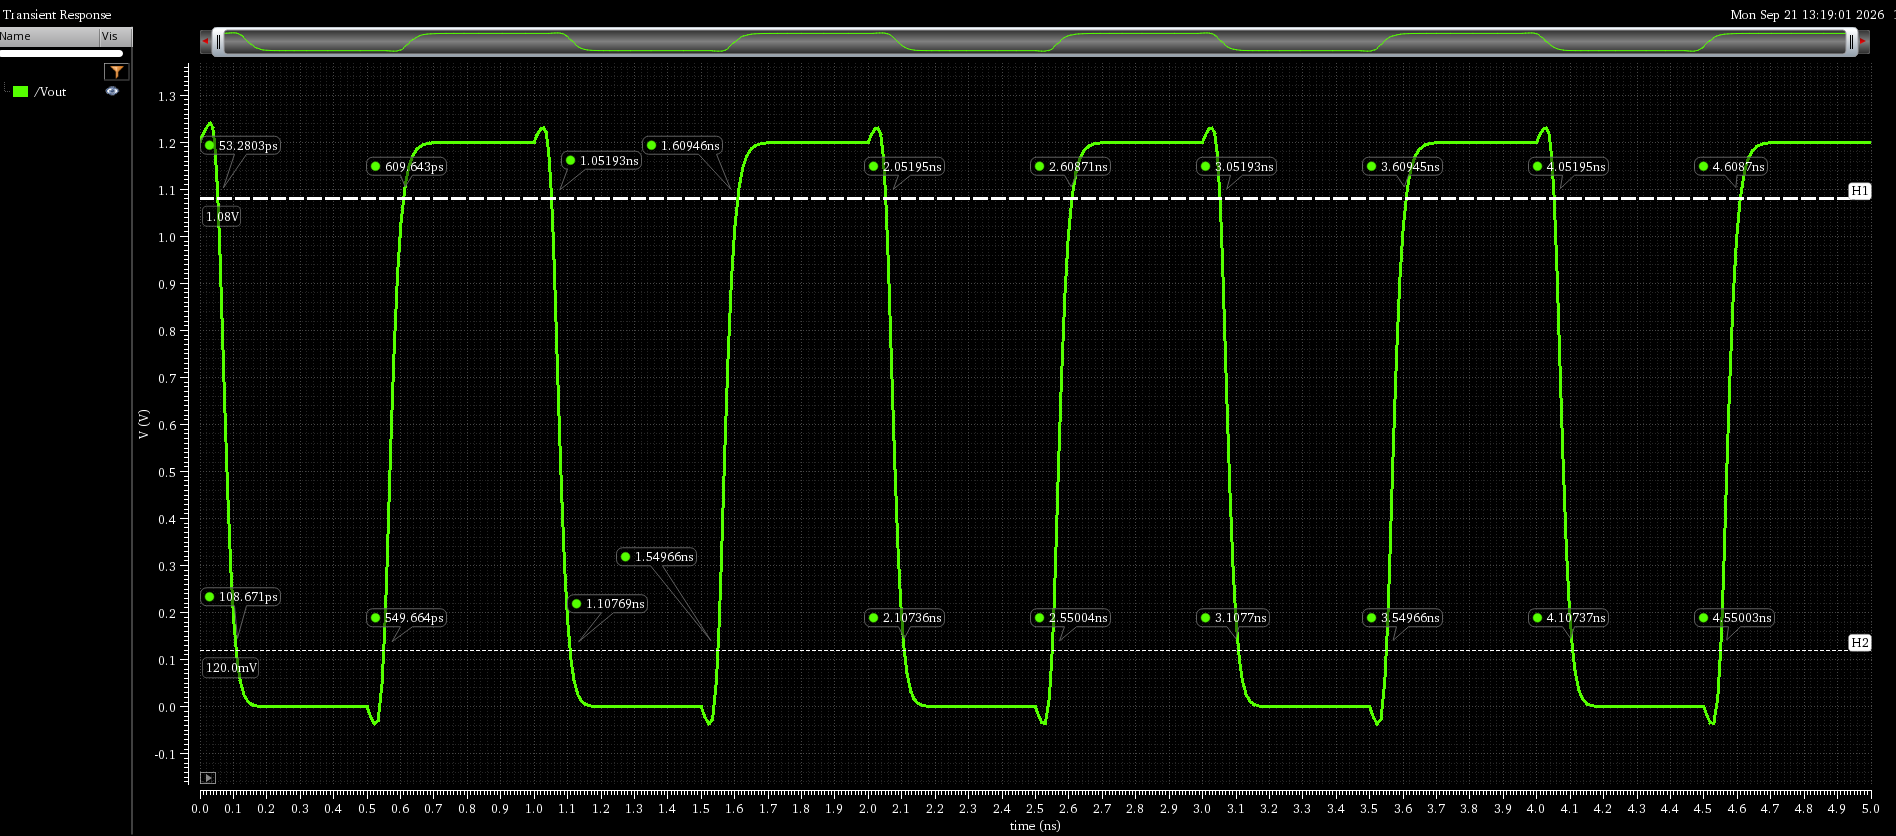
\includegraphics[width=\linewidth]{imagens/LVS_update/NAND_PEX_NORMAL_SIMULATION_TRISE_TFALL_10p90p.png}
    \caption{Medição PEX dos tempos de subida e de descida da NAND na condição típica, entre $120\,\mathrm{mV}$ e $1{,}08\,\mathrm{V}$.}
    \label{fig:nand-pex-normal-transicoes}
\end{figure}
\FloatBarrier
\begin{align}
    t_r &= (609{,}643-549{,}664)\,\mathrm{ps}
          =59{,}98\,\mathrm{ps}, \\
    t_f &= (1{,}10769-1{,}05193)\,\mathrm{ns}
          =55{,}76\,\mathrm{ps}.
\end{align}

\begin{figure}[!htbp]
    \centering
    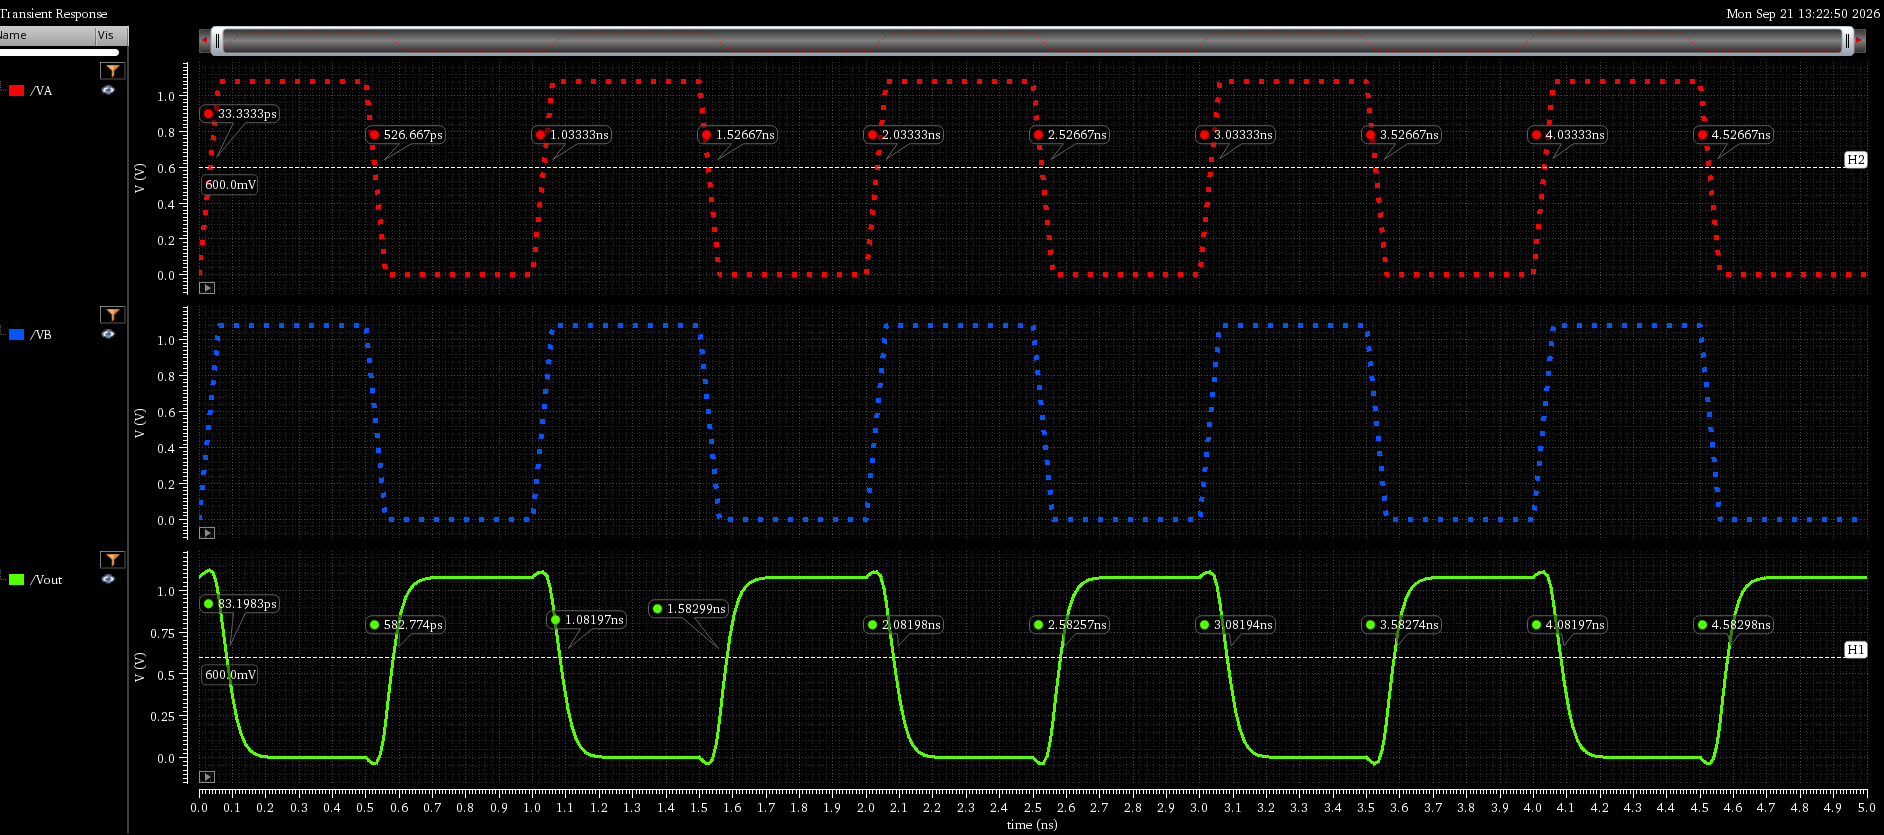
\includegraphics[width=\linewidth]{imagens/LVS_update/NAND_PEX_SLOW_SIMULATION_2.png}
    \caption{Simulação PEX da NAND no corner SLOW para a medição dos atrasos de propagação: $t_{pLH}=56{,}32\,\mathrm{ps}$ e $t_{pHL}=48{,}64\,\mathrm{ps}$.}
    \label{fig:nand-pex-slow}
\end{figure}

\FloatBarrier

No corner SLOW da Figura~\ref{fig:nand-pex-slow}, os cruzamentos indicados pelos marcadores resultam em
\begin{align}
    t_{pHL} &= (1{,}08197-1{,}03333)\,\mathrm{ns}
             =48{,}64\,\mathrm{ps}, \\
    t_{pLH} &= (1{,}58299-1{,}52667)\,\mathrm{ns}
             =56{,}32\,\mathrm{ps}, \\
    t_p &= \frac{t_{pLH}+t_{pHL}}{2}
          =52{,}48\,\mathrm{ps}.
\end{align}
Para as bordas da saída, utilizam-se os marcadores da Figura~\ref{fig:nand-pex-slow-transicoes}, posicionados em $108\,\mathrm{mV}$ e $972\,\mathrm{mV}$.
\begin{figure}[!htbp]
    \centering
    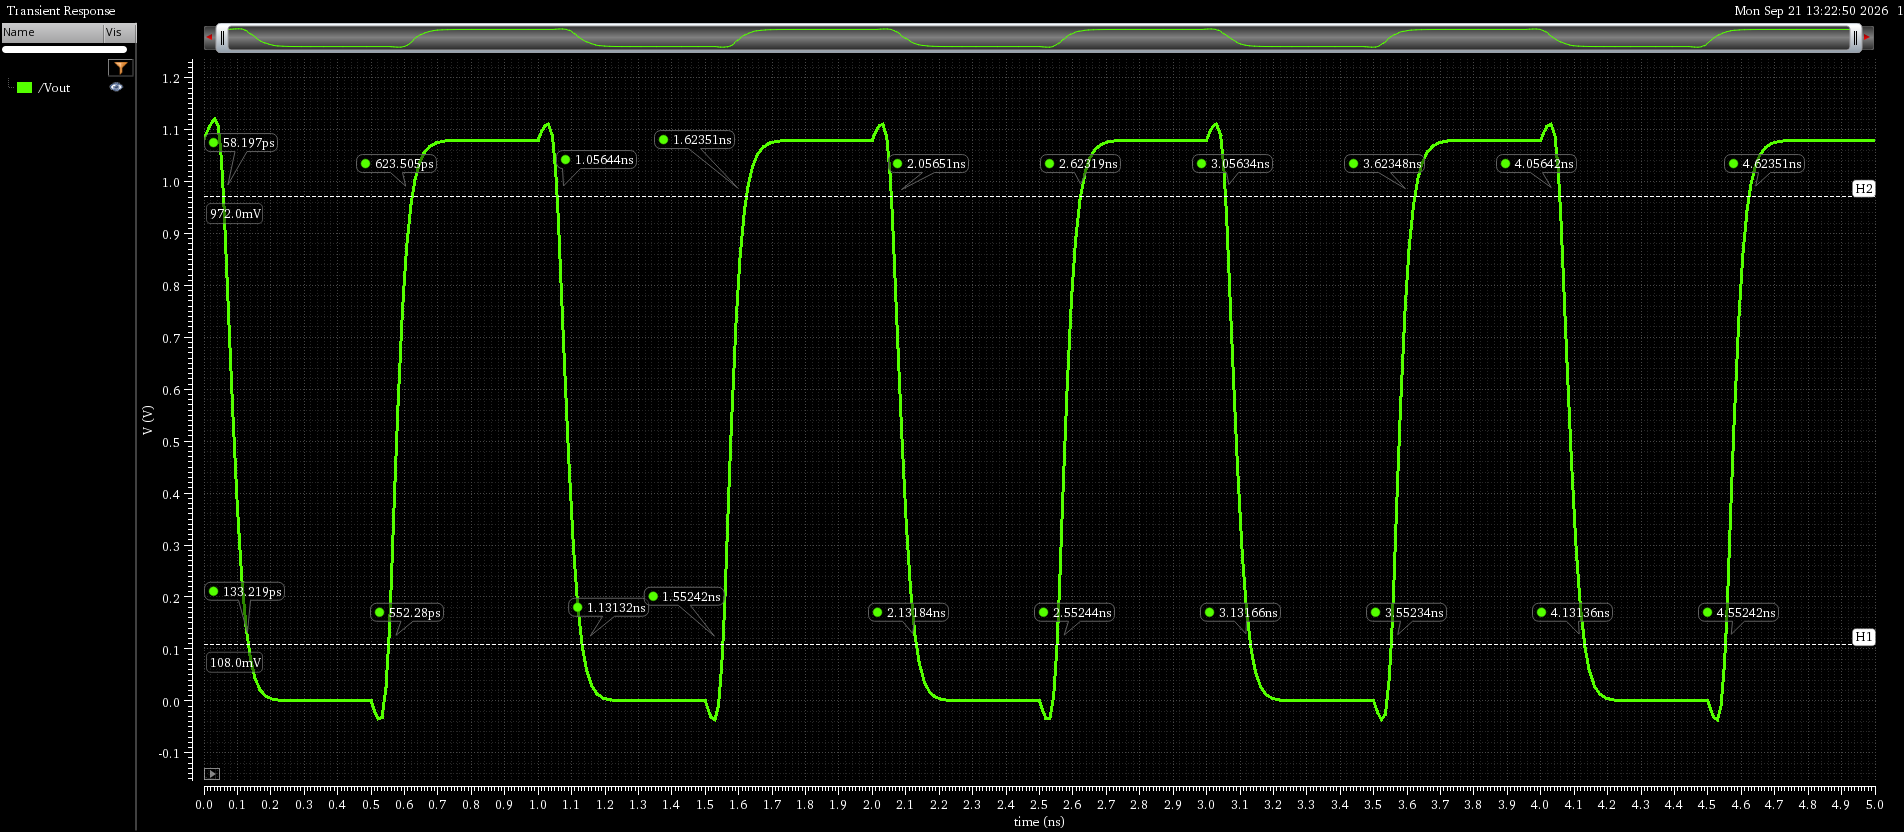
\includegraphics[width=\linewidth]{imagens/LVS_update/NAND_PEX_SLOW_SIMULATION_TRISE_TFALL_10p90p.png}
    \caption{Medição PEX dos tempos de subida e de descida da NAND no corner SLOW pelo critério de $10\%$--$90\%$.}
    \label{fig:nand-pex-slow-transicoes}
\end{figure}
\FloatBarrier
\begin{align}
    t_r &= (623{,}505-552{,}280)\,\mathrm{ps}
          =71{,}23\,\mathrm{ps}, \\
    t_f &= (1{,}13132-1{,}05644)\,\mathrm{ns}
          =74{,}88\,\mathrm{ps}.
\end{align}

\begin{figure}[!htbp]
    \centering
    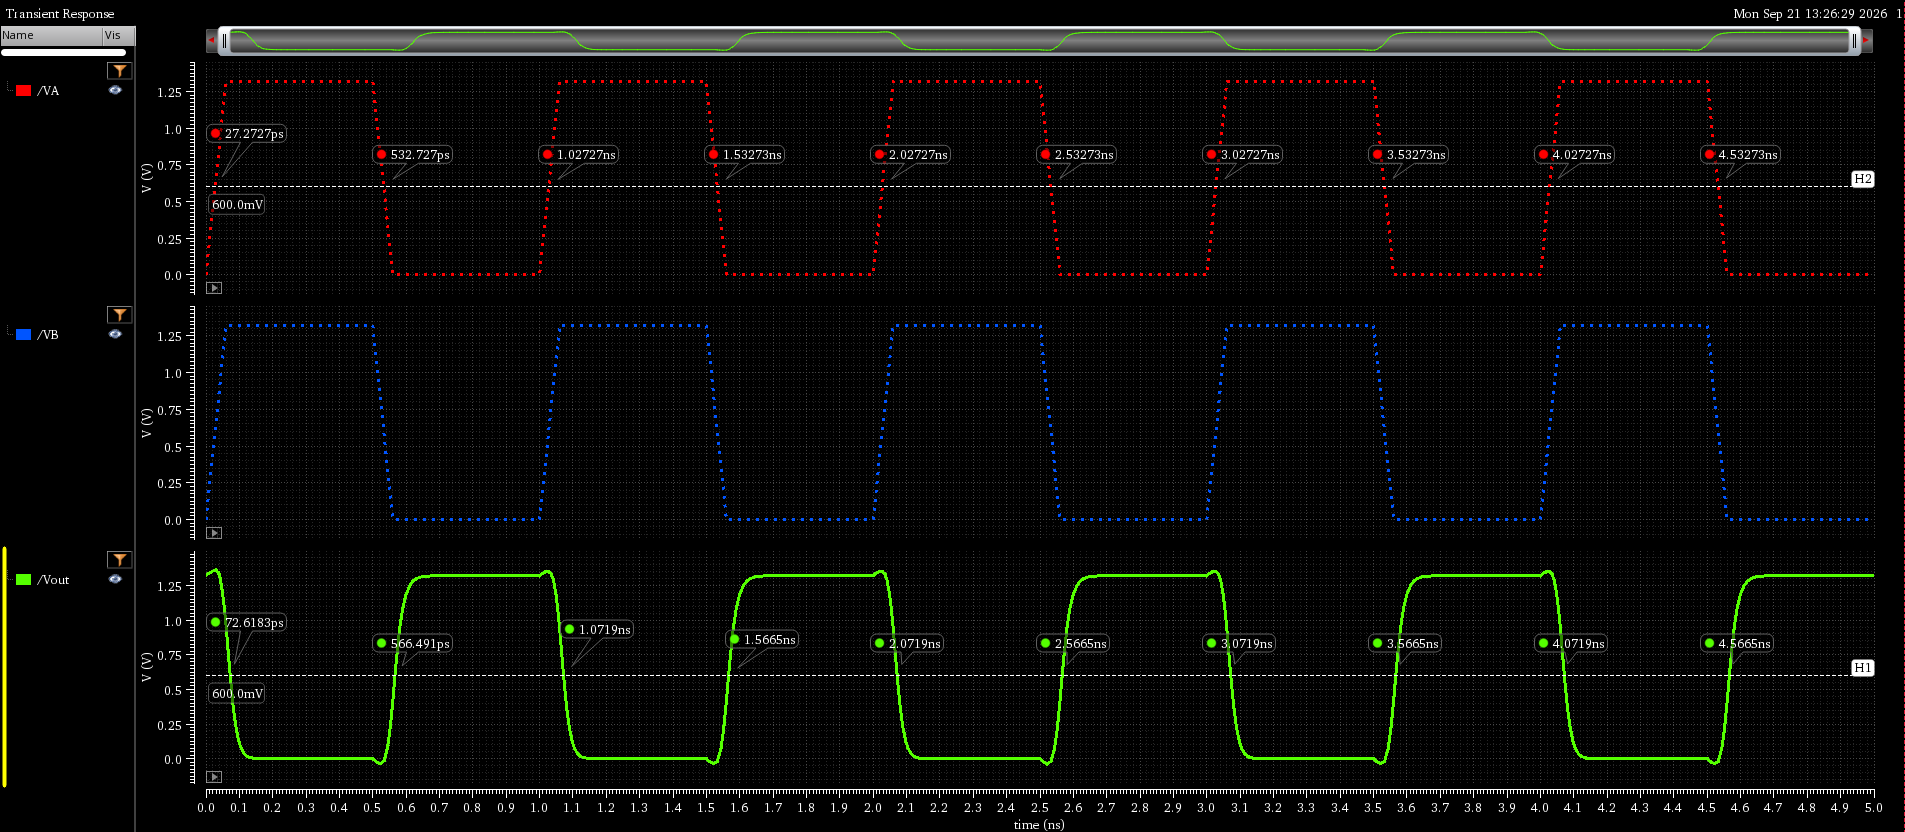
\includegraphics[width=\linewidth]{imagens/LVS_update/NAND_PEX_FAST_SIMULATION_2.png}
    \caption{Simulação PEX da NAND no corner FAST para a medição dos atrasos de propagação: $t_{pLH}=33{,}77\,\mathrm{ps}$ e $t_{pHL}=44{,}63\,\mathrm{ps}$.}
    \label{fig:nand-pex-fast}
\end{figure}

\FloatBarrier

No corner FAST da Figura~\ref{fig:nand-pex-fast}, obtêm-se
\begin{align}
    t_{pHL} &= (1{,}07190-1{,}02727)\,\mathrm{ns}
             =44{,}63\,\mathrm{ps}, \\
    t_{pLH} &= (1{,}56650-1{,}53273)\,\mathrm{ns}
             =33{,}77\,\mathrm{ps}, \\
    t_p &= \frac{t_{pLH}+t_{pHL}}{2}
          =39{,}20\,\mathrm{ps}.
\end{align}
Os tempos de transição são obtidos da Figura~\ref{fig:nand-pex-fast-transicoes}, com níveis de referência de $132\,\mathrm{mV}$ e $1{,}188\,\mathrm{V}$.
\begin{figure}[!htbp]
    \centering
    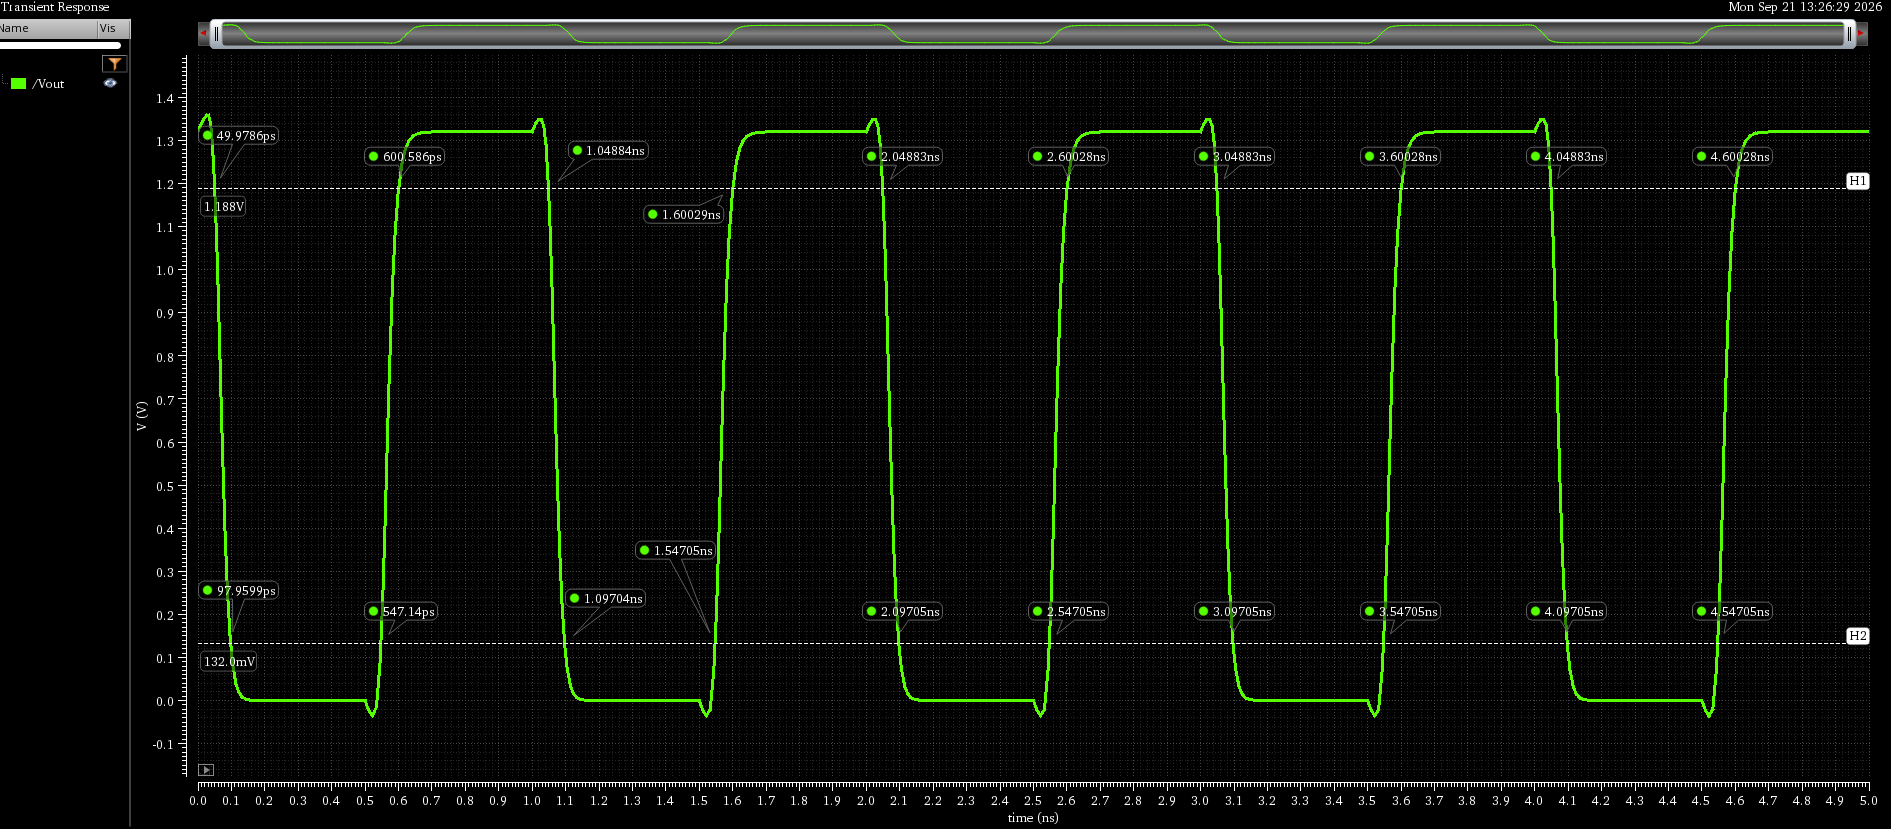
\includegraphics[width=\linewidth]{imagens/LVS_update/NAND_PEX_FAST_SIMULATION_TRISE_TFALL_10p90p.png}
    \caption{Medição PEX dos tempos de subida e de descida da NAND no corner FAST pelo critério de $10\%$--$90\%$.}
    \label{fig:nand-pex-fast-transicoes}
\end{figure}
\FloatBarrier
\begin{align}
    t_r &= (600{,}586-547{,}140)\,\mathrm{ps}
          =53{,}45\,\mathrm{ps}, \\
    t_f &= (1{,}09704-1{,}04884)\,\mathrm{ns}
          =48{,}20\,\mathrm{ps}.
\end{align}

\FloatBarrier

Os valores calculados para os três corners são reunidos e comparados aos resultados de esquemático na Tabela~\ref{tab:nand-esquematico-pex}.

Os atrasos médios e os tempos de transição pós-layout permanecem próximos dos valores de esquemático nos três corners. Os valores de $t_r$ e $t_f$ foram extraídos exclusivamente das capturas específicas de $10\%$--$90\%$, enquanto as imagens de simulação com marcadores em $600\,\mathrm{mV}$ foram utilizadas somente para $t_{pLH}$ e $t_{pHL}$. Nas simulações de esquemático dos corners SLOW e FAST, a referência dos atrasos era $50\%$ de cada alimentação; portanto, a comparação individual dos atrasos nesses corners deve considerar essa diferença de critério.

Nas duas últimas colunas da tabela, a variação causada pela inclusão dos parasitas é calculada, para cada corner, por
\begin{equation}
    \Delta t_p=t_{p,\text{PEX}}-t_{p,\text{esquemático}},
    \qquad
    \Delta t_p(\%)=\frac{\Delta t_p}{t_{p,\text{esquemático}}}\,100\%.
\end{equation}

\begin{table}[!htbp]
    \centering
    \small
    \caption{Comparação entre as simulações de esquemático e PEX da porta NAND.}
    \label{tab:nand-esquematico-pex}
    \resizebox{\linewidth}{!}{%
    \begin{tabular}{llccccccc}
        \hline
        Condição & Modelo & $t_{pLH}$ ($\mathrm{ps}$) & $t_{pHL}$ ($\mathrm{ps}$) & $t_p$ ($\mathrm{ps}$) & $t_r$ ($\mathrm{ps}$) & $t_f$ ($\mathrm{ps}$) & $\Delta t_p$ ($\mathrm{ps}$) & $\Delta t_p$ ($\%$) \\
        \hline
        Típica & Esquemático & $43{,}07$ & $45{,}05$ & $44{,}06$ & $59{,}66$ & $55{,}42$ & -- & -- \\
        Típica & PEX         & $43{,}07$ & $45{,}06$ & $44{,}07$ & $59{,}98$ & $55{,}76$ & $+0{,}01$ & $+0{,}02$ \\
        SLOW   & Esquemático & $48{,}83$ & $56{,}11$ & $52{,}47$ & $70{,}75$ & $75{,}34$ & -- & -- \\
        SLOW   & PEX         & $56{,}32$ & $48{,}64$ & $52{,}48$ & $71{,}23$ & $74{,}88$ & $+0{,}01$ & $+0{,}02$ \\
        FAST   & Esquemático & $38{,}75$ & $39{,}71$ & $39{,}23$ & $53{,}24$ & $48{,}21$ & -- & -- \\
        FAST   & PEX         & $33{,}77$ & $44{,}63$ & $39{,}20$ & $53{,}45$ & $48{,}20$ & $-0{,}03$ & $-0{,}08$ \\
        \hline
    \end{tabular}%
    }
\end{table}

\FloatBarrier


\section{Cálculo dos parâmetros da porta NOR}

A porta NOR de duas entradas foi implementada em lógica CMOS estática no Cadence Virtuoso, conforme a Figura~\ref{fig:nor-esquematico}. Novamente, observa-se que na condição pedida para simulações com $A = B$, a porta se comporta como um inversor.

Ao contrário da NAND, a NOR utiliza dois PMOS em série entre a alimentação e a saída e dois NMOS em paralelo entre a saída e o terra. A saída assume nível alto somente para $A=B=0$, quando ambos os PMOS conduzem e os dois NMOS estão cortados. Se pelo menos uma entrada estiver em nível alto, o NMOS correspondente estabelece um caminho de descarga e a rede PMOS tem seu caminho de condução interrompido, levando a saída ao nível baixo.

\begin{figure}[!htbp]
    \centering
    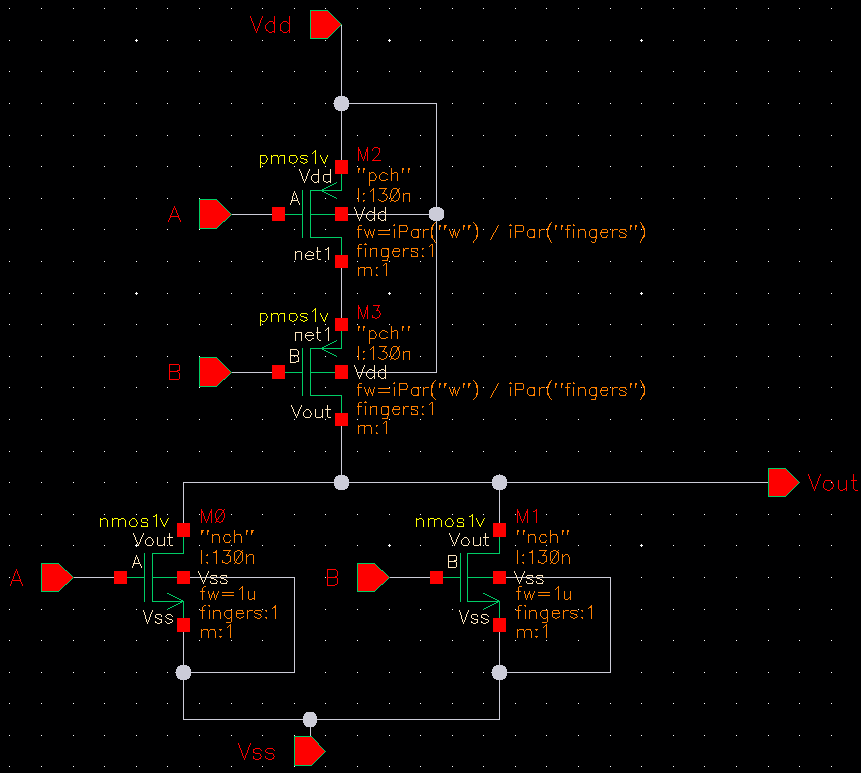
\includegraphics[width=0.82\linewidth]{imagens/NOR_schematic.png}
    \caption{Esquemático da porta NOR de duas entradas, com PMOS em série e NMOS em paralelo.}
    \label{fig:nor-esquematico}
\end{figure}

Os quatro transistores apresentam comprimento de canal de $L=130\,\mathrm{nm}$, um único finger e multiplicidade unitária. Cada NMOS possui largura de $W_n=2\,\mu\mathrm{m}$, enquanto a largura dos PMOS é novamente parametrizada. A associação em série dos PMOS torna o dimensionamento da rede de carga particularmente importante para equilibrar os atrasos de subida e de descida.

O circuito de teste da Figura~\ref{fig:nor-testbench} utiliza alimentação de $V_{DD}=1{,}2\,\mathrm{V}$, terra em $0\,\mathrm{V}$ e capacitância de carga de $C_L=10\,\mathrm{fF}$. As duas fontes pulsadas variam entre $0$ e $1{,}2\,\mathrm{V}$, com tempo de subida configurado em $60\,\mathrm{ps}$. Essas condições de alimentação e carga são as mesmas utilizadas no teste da NAND, embora o dimensionamento dos transistores seja diferente.

\begin{figure}[!htbp]
    \centering
    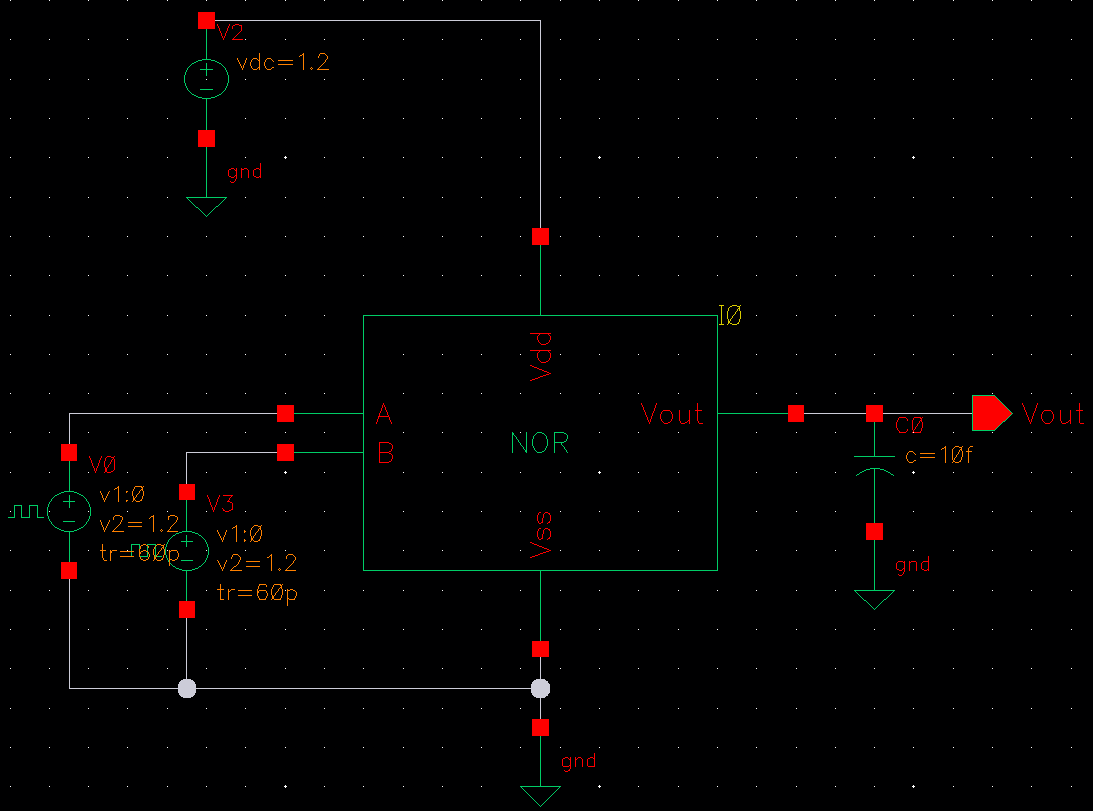
\includegraphics[width=0.72\linewidth]{imagens/NOR_tb_schematic.PNG}
    \caption{Circuito de teste da porta NOR, com duas entradas pulsadas, alimentação de $1{,}2\,\mathrm{V}$ e carga de $10\,\mathrm{fF}$.}
    \label{fig:nor-testbench}
\end{figure}

\subsection{Configuração da simulação no ADE}

A Figura~\ref{fig:nor-ade} apresenta a configuração do ADE para a NOR. A análise transitória é realizada de $0$ a $5\,\mathrm{ns}$, à temperatura de $27\,^{\circ}\mathrm{C}$. Foram selecionados os sinais \texttt{Vout}, \texttt{A} e \texttt{B}, além das expressões para os atrasos de propagação \texttt{tplh} e \texttt{tphl}.

\begin{figure}[!htbp]
    \centering
    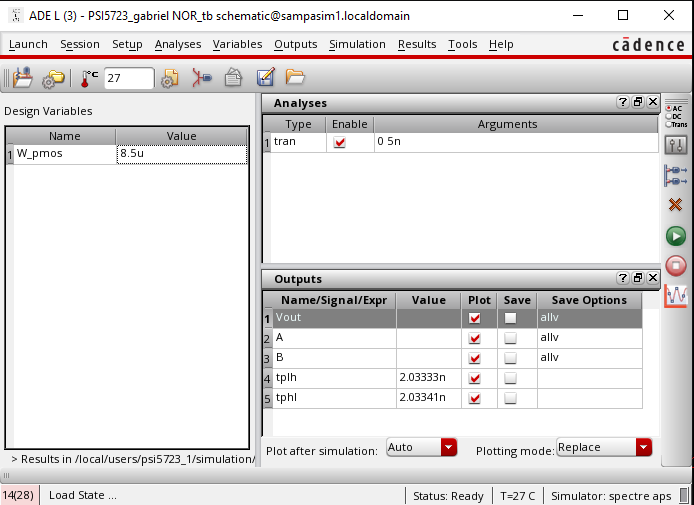
\includegraphics[width=0.80\linewidth]{imagens/NOR_tb_ADE.PNG}
    \caption{Configuração da NOR no ADE, com $W_p=8{,}5\,\mu\mathrm{m}$ e análise transitória até $5\,\mathrm{ns}$. Os valores das expressões de atraso exigem a verificação discutida no texto.}
    \label{fig:nor-ade}
\end{figure}

\subsection{Varredura da largura dos transistores PMOS}

Novamente, utilizamos a ferramenta Parametric Analysis para realizar a varredura da variável \texttt{W\_pmos}. A Figura~\ref{fig:nor-atrasos-varredura} mostra as grandezas \texttt{tplh} e \texttt{tphl} em função de \texttt{W\_pmos}, no intervalo exibido de $4$ a $9\,\mu\mathrm{m}$. A curva de \texttt{tplh} diminui com a largura dos PMOS, enquanto a de \texttt{tphl} aumenta. Esse comportamento é compatível, respectivamente, com o fortalecimento da rede de carga e com o aumento das capacitâncias dos dispositivos conectados à saída.

\begin{figure}[!htbp]
    \centering
    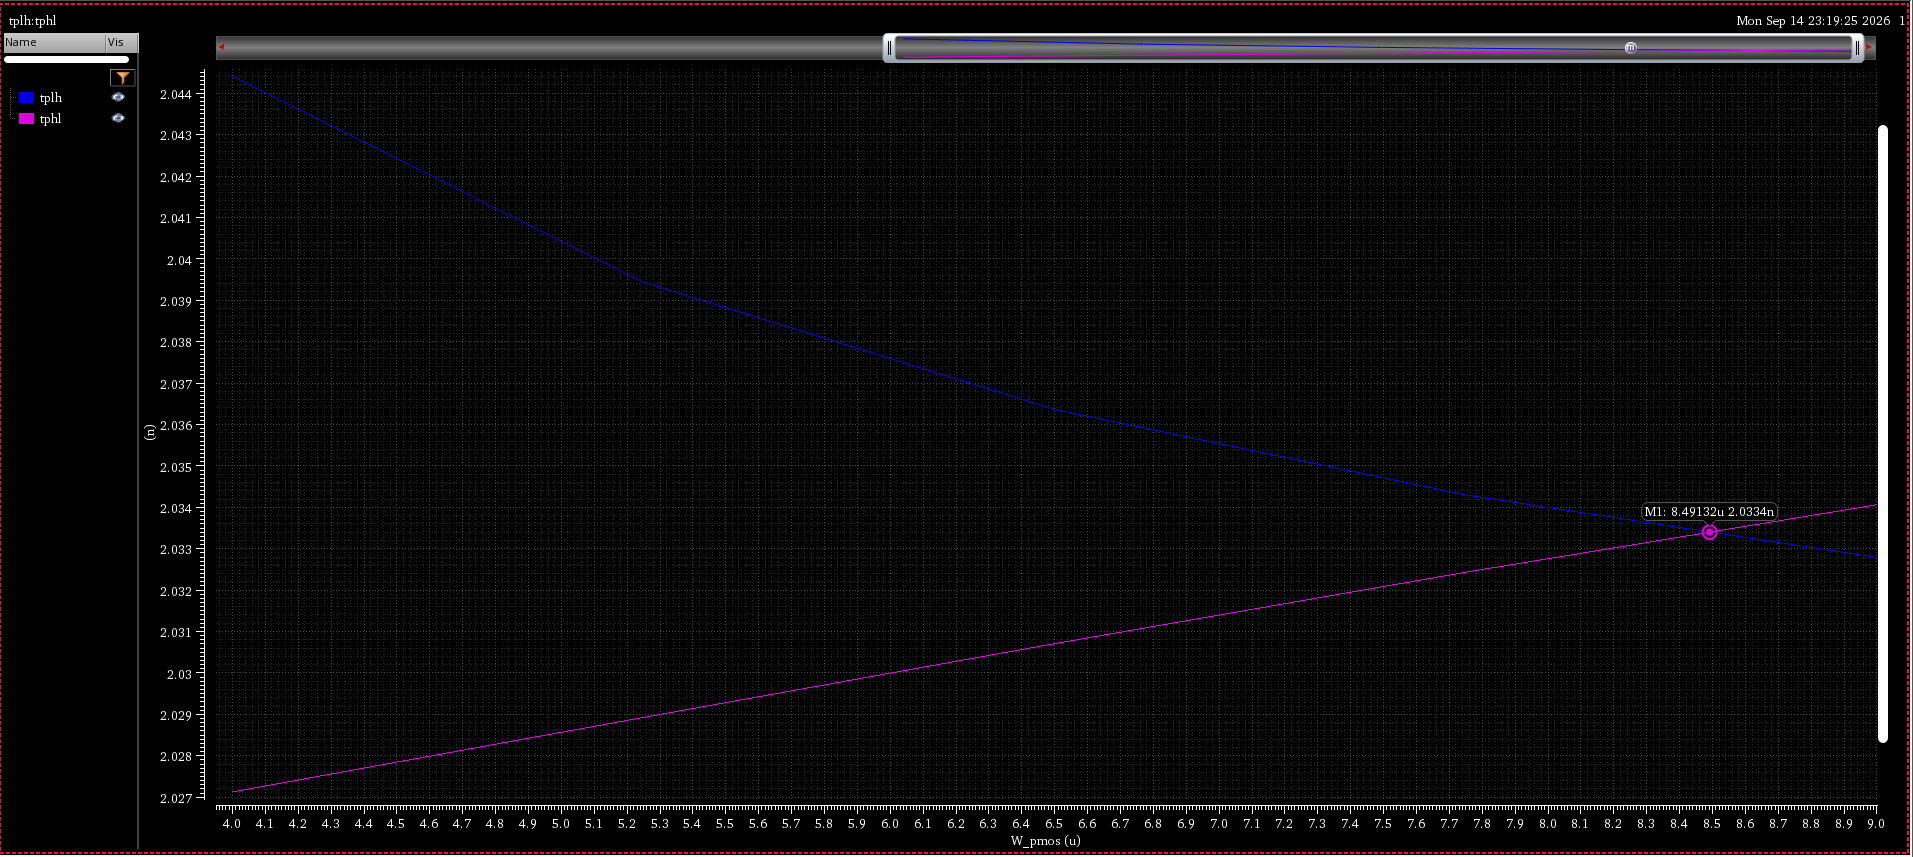
\includegraphics[width=\linewidth]{imagens/NOR_tb_tplh_tphl.PNG}
    \caption{Varredura da largura dos PMOS da NOR: expressão \texttt{tplh} em azul e \texttt{tphl} em magenta. O marcador próximo à interseção indica $W_p\approx8{,}5\,\mu\mathrm{m}$. A escala vertical é discutida no texto.}
    \label{fig:nor-atrasos-varredura}
\end{figure}

O marcador indica uma interseção próxima de $W_p=8{,}5\,\mu\mathrm{m}$ no ADE para aproximar os dois atrasos. Essa largura corresponde a $W_p/W_n=4{,}25$ por transistor.

\begin{tcolorbox}[
    title={Estimativa teórica para a largura dos PMOS da NOR},
    colback=bleu303pale,
    colframe=bleu303,
    fonttitle=\bfseries
]

Na condição simulada $A=B$, o caminho de carga é formado pelos dois PMOS em série e na descarga os dois NMOS conduzem em paralelo durante a descarga. Dessa forma, calculam-se os tempos de carga e descarga com $R_{p,\text{eq}} = 2R_p$ e $R_{n,\text{eq}} = \frac{R_n}{2}$ respectivamente

\begin{align}
    t_{pLH} &= 0,69 (2R_p) C_L \\
    t_{pHL} &= 0,69 \left(\frac{R_n}{2}\right) C_L
\end{align}

A igualdade $t_{pLH} = t_{pHL}$ ocorre quando
\begin{equation}
    4\frac{R_p}{R_n} = 1 \iff 4 \left(\frac{W_n}{W_p}\right) \left(\frac{\mu_n}{\mu_p}\right) = 1 \iff W_p = 4  \left(\frac{\mu_n}{\mu_p}\right) W_n
\end{equation}

Para $W_n=1\,\mu\mathrm{m}$ e adotando $\frac{\mu_n}{\mu_p} \approx 2$, a estimativa é $W_p\approx 8 \,\mu\mathrm{m}$. Assim, o valor experimental $W_p\approx8{,}5\,\mu\mathrm{m}$ está de próximo do dimensionamento teórico da NOR.
\end{tcolorbox}

\subsection{Atrasos de propagação na análise transitória}

A Figura~\ref{fig:nor-marcadores} apresenta as formas de onda com marcadores horizontais em $600\,\mathrm{mV}$, correspondentes a $50\%$ de $V_{DD}$. As entradas \texttt{/A} e \texttt{/B} comutam simultaneamente. A saída desce quando ambas sobem e retorna ao nível alto quando ambas descem, comportamento coerente com a função NOR para as combinações $00$ e $11$. %Esse teste não verifica isoladamente as combinações $01$ e $10$, nem os atrasos de cada entrada com a outra mantida em nível baixo.

\begin{figure}[!htbp]
    \centering
    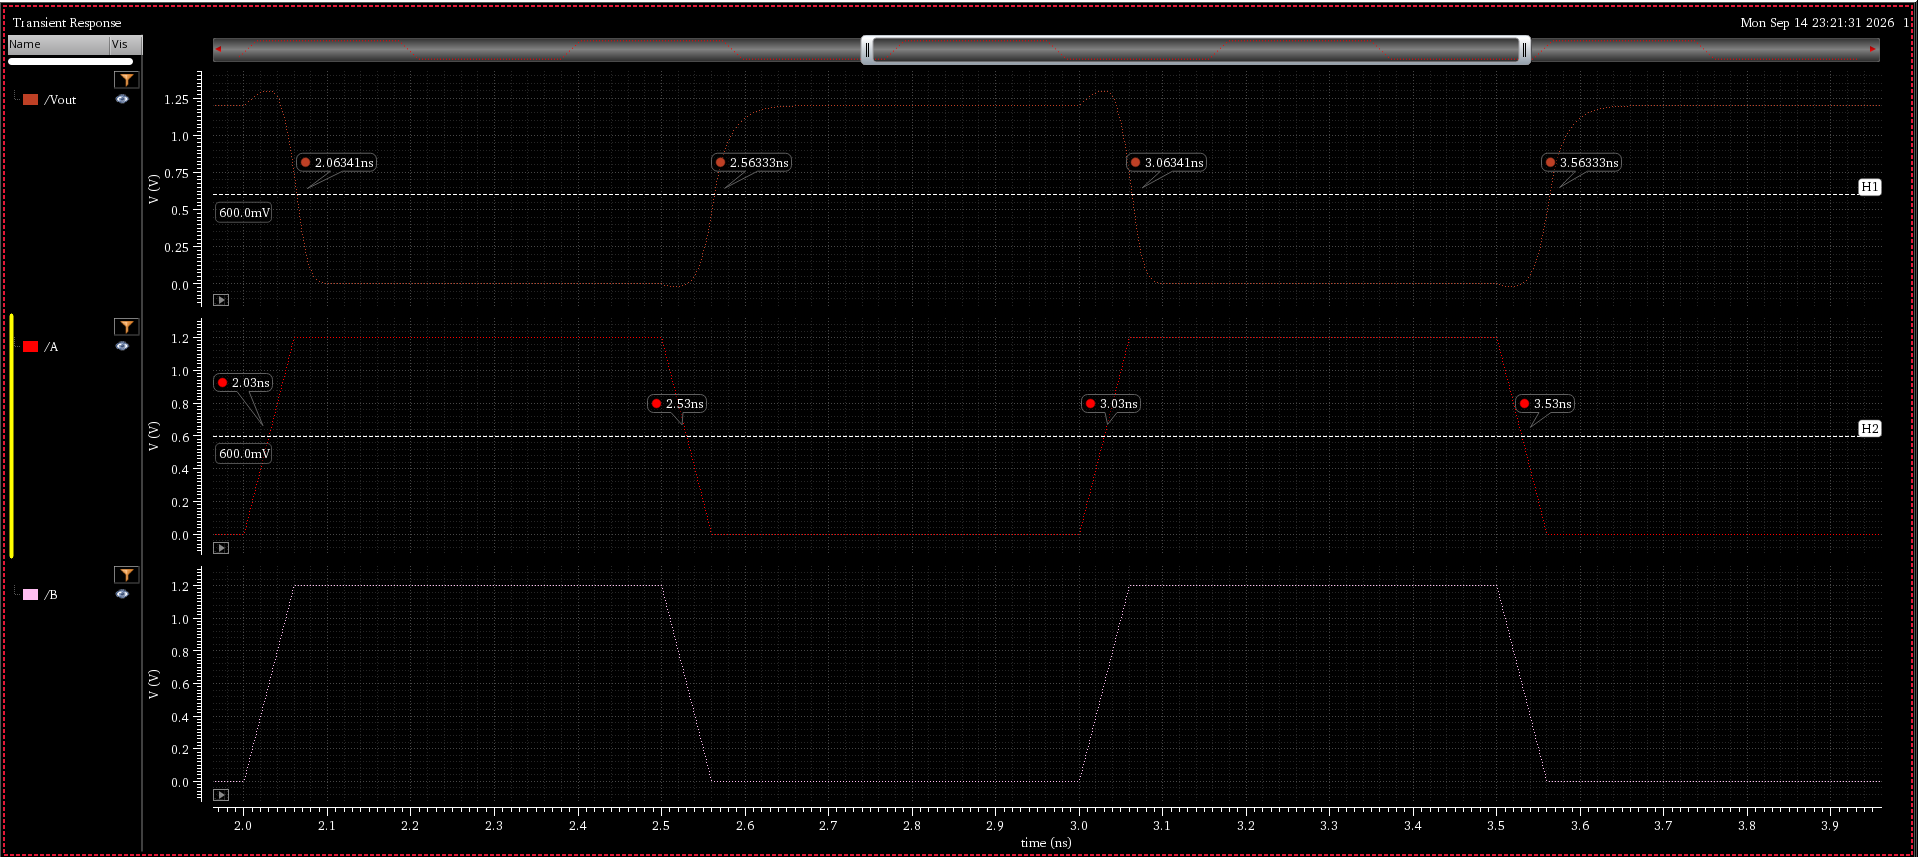
\includegraphics[width=\linewidth]{imagens/NOR_horizontal_markers.PNG}
    \caption{Formas de onda da NOR e marcadores em $600\,\mathrm{mV}$ para a medição dos atrasos entre transições correspondentes de entrada e saída.}
    \label{fig:nor-marcadores}
\end{figure}

Utilizando o mesmo critério de medição de $50\%$ empregado para a NAND, obtêm-se
\begin{align}
    t_{pHL} &= (2{,}06341-2{,}03000)\,\mathrm{ns}
             = 33{,}41\,\mathrm{ps}, \\
    t_{pLH} &= (2{,}56333-2{,}53000)\,\mathrm{ns}
             = 33{,}33\,\mathrm{ps}.
\end{align}
Consequentemente, o atraso médio de propagação é
\begin{equation}
    t_p=\frac{t_{pLH}+t_{pHL}}{2}=33{,}37\,\mathrm{ps}.
\end{equation}
Os marcadores do ciclo seguinte, em $3{,}03$ e $3{,}06341\,\mathrm{ns}$ para a descida da saída e em $3{,}53$ e $3{,}56333\,\mathrm{ns}$ para a subida, reproduzem os mesmos atrasos na precisão apresentada. A diferença entre $t_{pHL}$ e $t_{pLH}$ é de apenas $0{,}08\,\mathrm{ps}$, indicando bom equilíbrio nessa condição de teste. São essas diferenças entre os marcadores, e não os valores absolutos exibidos pelas expressões do ADE, que fundamentam o resumo dos resultados.

\subsection{Tempos de subida e de descida}

A Figura~\ref{fig:nor-subida-descida} apresenta as medições das bordas da saída. A ferramenta utiliza o critério de $10\%$--$90\%$, com níveis de referência explicitamente definidos em $0$ e $1{,}2\,\mathrm{V}$; os limiares são, portanto, $0{,}12$ e $1{,}08\,\mathrm{V}$. Essa definição evita que o pequeno pico acima de $V_{DD}$, visível antes da descida, altere os limiares por uma escolha automática baseada no máximo da forma de onda.

\begin{figure}[!htbp]
    \centering
    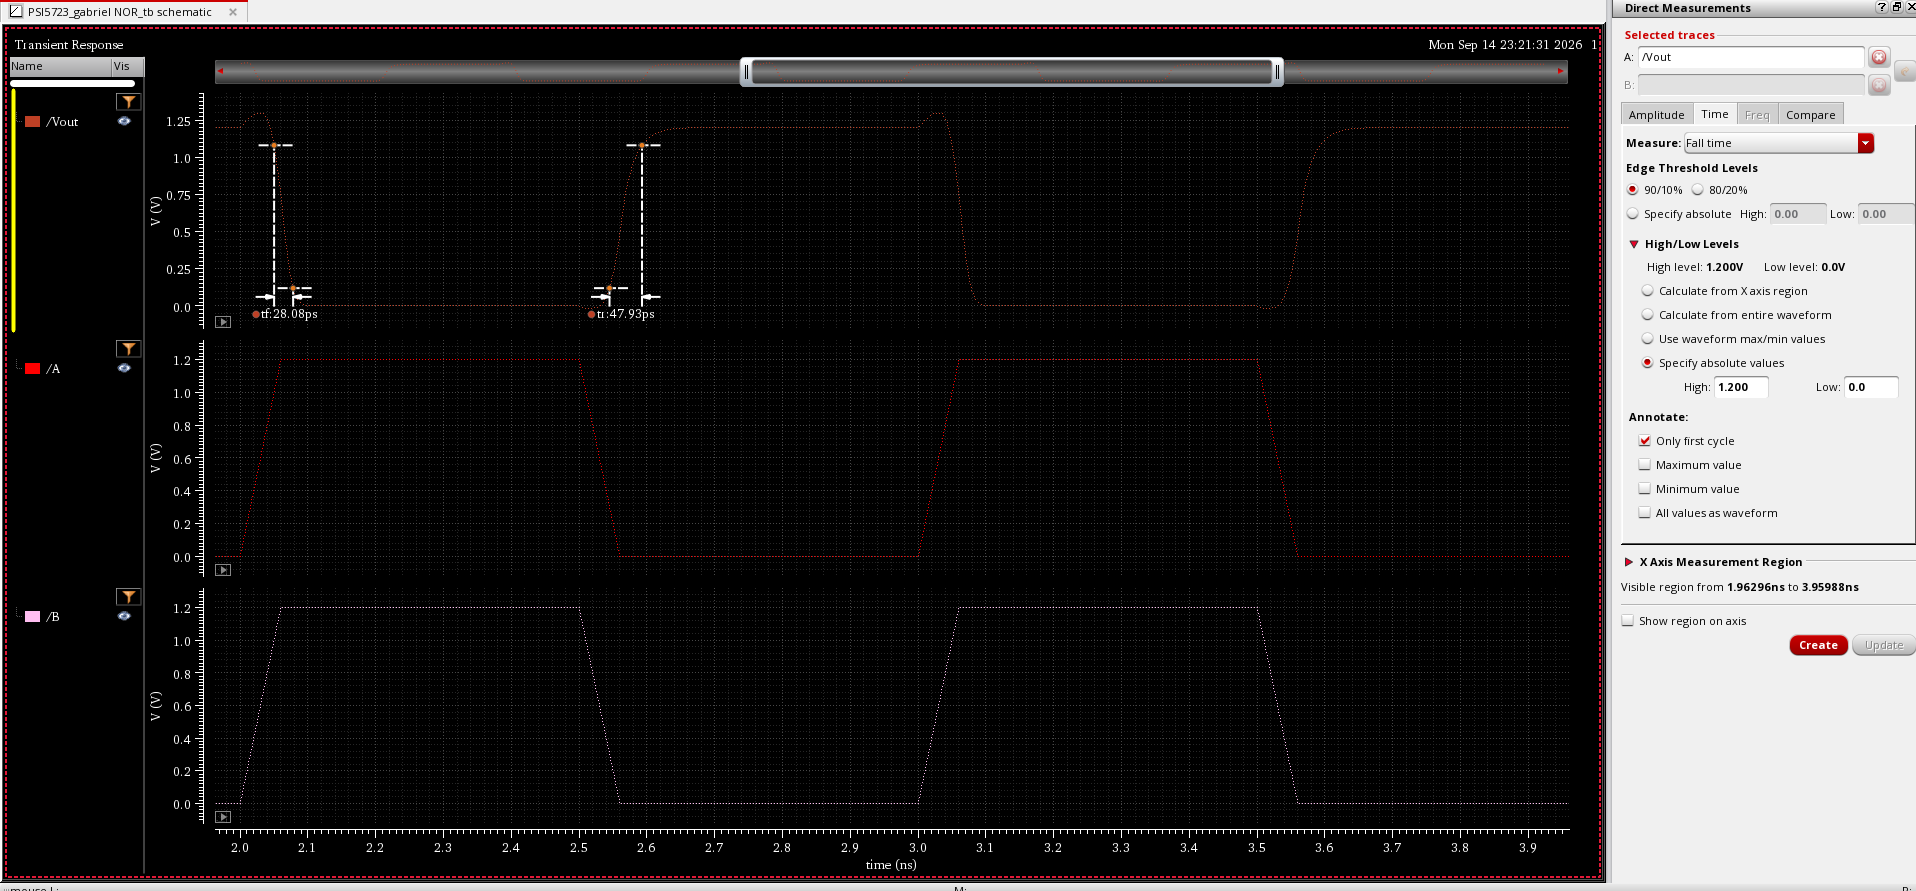
\includegraphics[width=\linewidth]{imagens/NOR_rise_fall_time.PNG}
    \caption{Medição das bordas da saída da NOR pelo critério de $10\%$--$90\%$, com $t_r=47{,}93\,\mathrm{ps}$ e $t_f=28{,}08\,\mathrm{ps}$.}
    \label{fig:nor-subida-descida}
\end{figure}

Os marcadores fornecem $t_r=47{,}93\,\mathrm{ps}$ e $t_f=28{,}08\,\mathrm{ps}$. A subida é mais lenta que a descida, apesar de os atrasos de propagação medidos a $50\%$ serem praticamente iguais. Não há contradição: o equilíbrio de $t_{pLH}$ e $t_{pHL}$ não implica igualdade dos intervalos necessários para percorrer de $10\%$ a $90\%$ da excursão de saída.

\begin{table}[!htbp]
    \centering
    \caption{Resumo das medições transitórias da NOR, com $W_p=8{,}5\,\mu\mathrm{m}$, $W_n=2\,\mu\mathrm{m}$, $V_{DD}=1{,}2\,\mathrm{V}$ e $C_L=10\,\mathrm{fF}$. Os atrasos são calculados pelos marcadores das formas de onda.}
    \label{tab:nor-tempos}
    \begin{tabular}{lcc}
        \hline
        Grandeza & Critério de medição & Valor ($\mathrm{ps}$) \\
        \hline
        Atraso de subida, $t_{pLH}$ & Entrada--saída, $50\%$ & $33{,}33$ \\
        Atraso de descida, $t_{pHL}$ & Entrada--saída, $50\%$ & $33{,}41$ \\
        Atraso médio, $t_p$ & $(t_{pLH}+t_{pHL})/2$ & $33{,}37$ \\
        Tempo de subida, $t_r$ & Saída, $10\% \rightarrow 90\%$ & $47{,}93$ \\
        Tempo de descida, $t_f$ & Saída, $90\% \rightarrow 10\%$ & $28{,}08$ \\
        \hline
    \end{tabular}
\end{table}

\FloatBarrier

A Tabela~\ref{tab:nor-tempos} reúne os resultados da NOR. Comparando-a com a Tabela~\ref{tab:nand-tempos}, o atraso médio da NOR é menor no teste apresentado, mas seus transistores também possuem larguras maiores. Logo, a comparação caracteriza os dois dimensionamentos adotados, e não uma vantagem universal da topologia NOR. Os resultados são de esquemático, sem caracterização de layout extraído nesta etapa, e não estabelecem o pior caso entre todas as transições possíveis das entradas.

\subsection{Simulação nos corners SLOW e FAST}

A porta NOR também foi simulada nos corners SLOW e FAST, mantendo-se $W_p=8{,}5\,\mu\mathrm{m}$ e a capacitância de carga de $10\,\mathrm{fF}$. As Figuras~\ref{fig:nor-slow-config} e~\ref{fig:nor-fast-config} apresentam as configurações das duas simulações. Os atrasos dos corners foram calculados diretamente pelas diferenças entre os marcadores das entradas e da saída. Os níveis de referência adotados são $540\,\mathrm{mV}$ para o corner SLOW e $660\,\mathrm{mV}$ para o corner FAST, correspondentes a $50\%$ das respectivas tensões de alimentação.

\begin{figure}[!htbp]
    \centering
    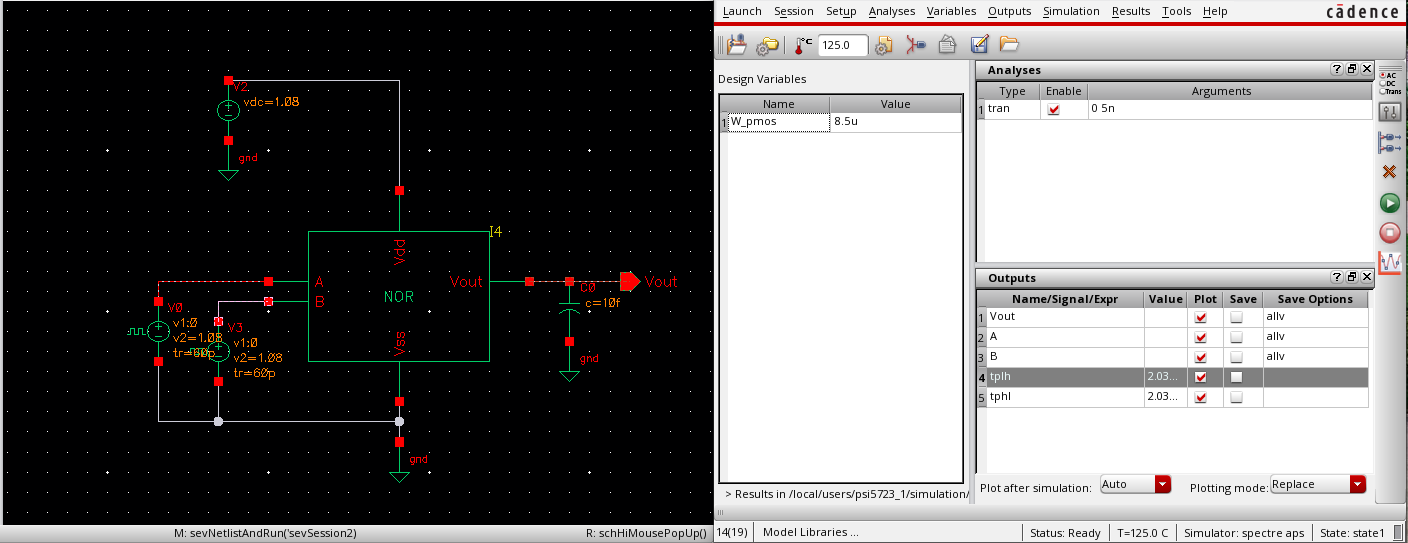
\includegraphics[width=\linewidth]{imagens/NOR_SLOW.PNG}
    \caption{Configuração da simulação da NOR no corner SLOW (WCS), com $W_p=8{,}5\,\mu\mathrm{m}$, $V_{DD}=1{,}08\,\mathrm{V}$ e temperatura de $125\,^{\circ}\mathrm{C}$.}
    \label{fig:nor-slow-config}
\end{figure}

\begin{figure}[!htbp]
    \centering
    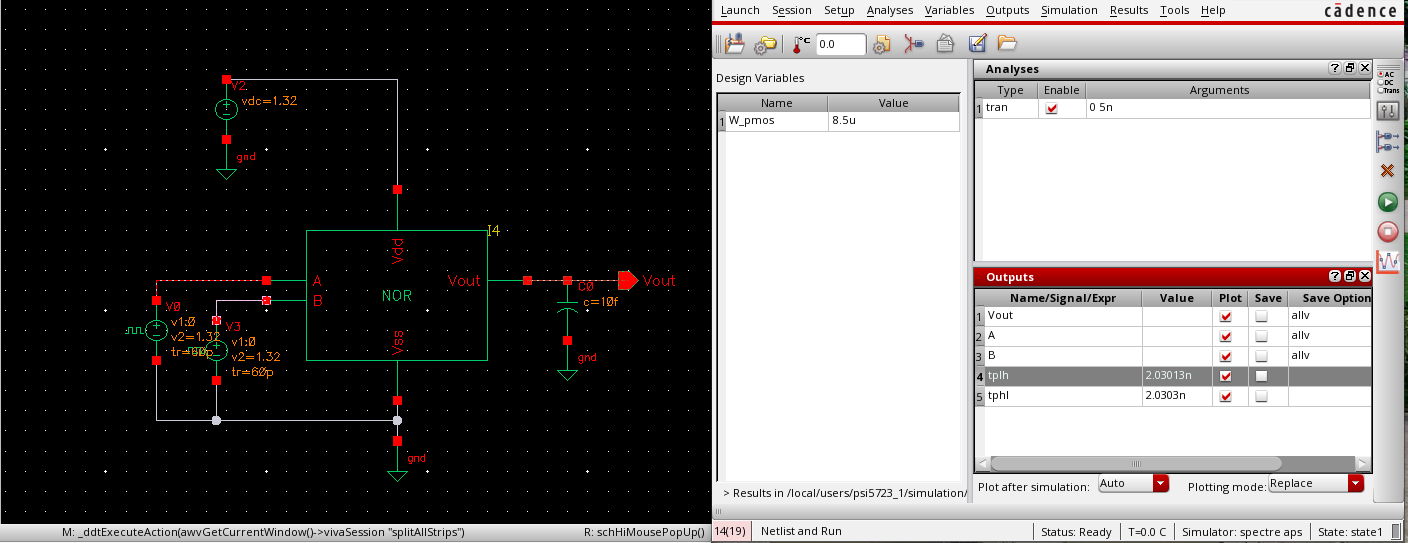
\includegraphics[width=\linewidth]{imagens/NOR_FAST.PNG}
    \caption{Configuração da simulação da NOR no corner FAST (WCP), com $W_p=8{,}5\,\mu\mathrm{m}$, $V_{DD}=1{,}32\,\mathrm{V}$ e temperatura de $0\,^{\circ}\mathrm{C}$.}
    \label{fig:nor-fast-config}
\end{figure}

\subsubsection{Atrasos de propagação}

As formas de onda e os marcadores utilizados para calcular os atrasos são mostrados nas Figuras~\ref{fig:nor-slow-atrasos} e~\ref{fig:nor-fast-atrasos}. No corner SLOW, a entrada cruza $540\,\mathrm{mV}$ em $2{,}03000\,\mathrm{ns}$ durante a subida, e a saída cruza o mesmo nível em $2{,}06985\,\mathrm{ns}$ durante a descida. Para a transição oposta, os cruzamentos ocorrem em $2{,}53000\,\mathrm{ns}$ e $2{,}56826\,\mathrm{ns}$. Portanto,
\begin{align}
    t_{pHL,\mathrm{SLOW}} &= (2{,}06985-2{,}03000)\,\mathrm{ns}
                            = 39{,}85\,\mathrm{ps}, \\
    t_{pLH,\mathrm{SLOW}} &= (2{,}56826-2{,}53000)\,\mathrm{ns}
                            = 38{,}26\,\mathrm{ps}.
\end{align}

\begin{figure}[!htbp]
    \centering
    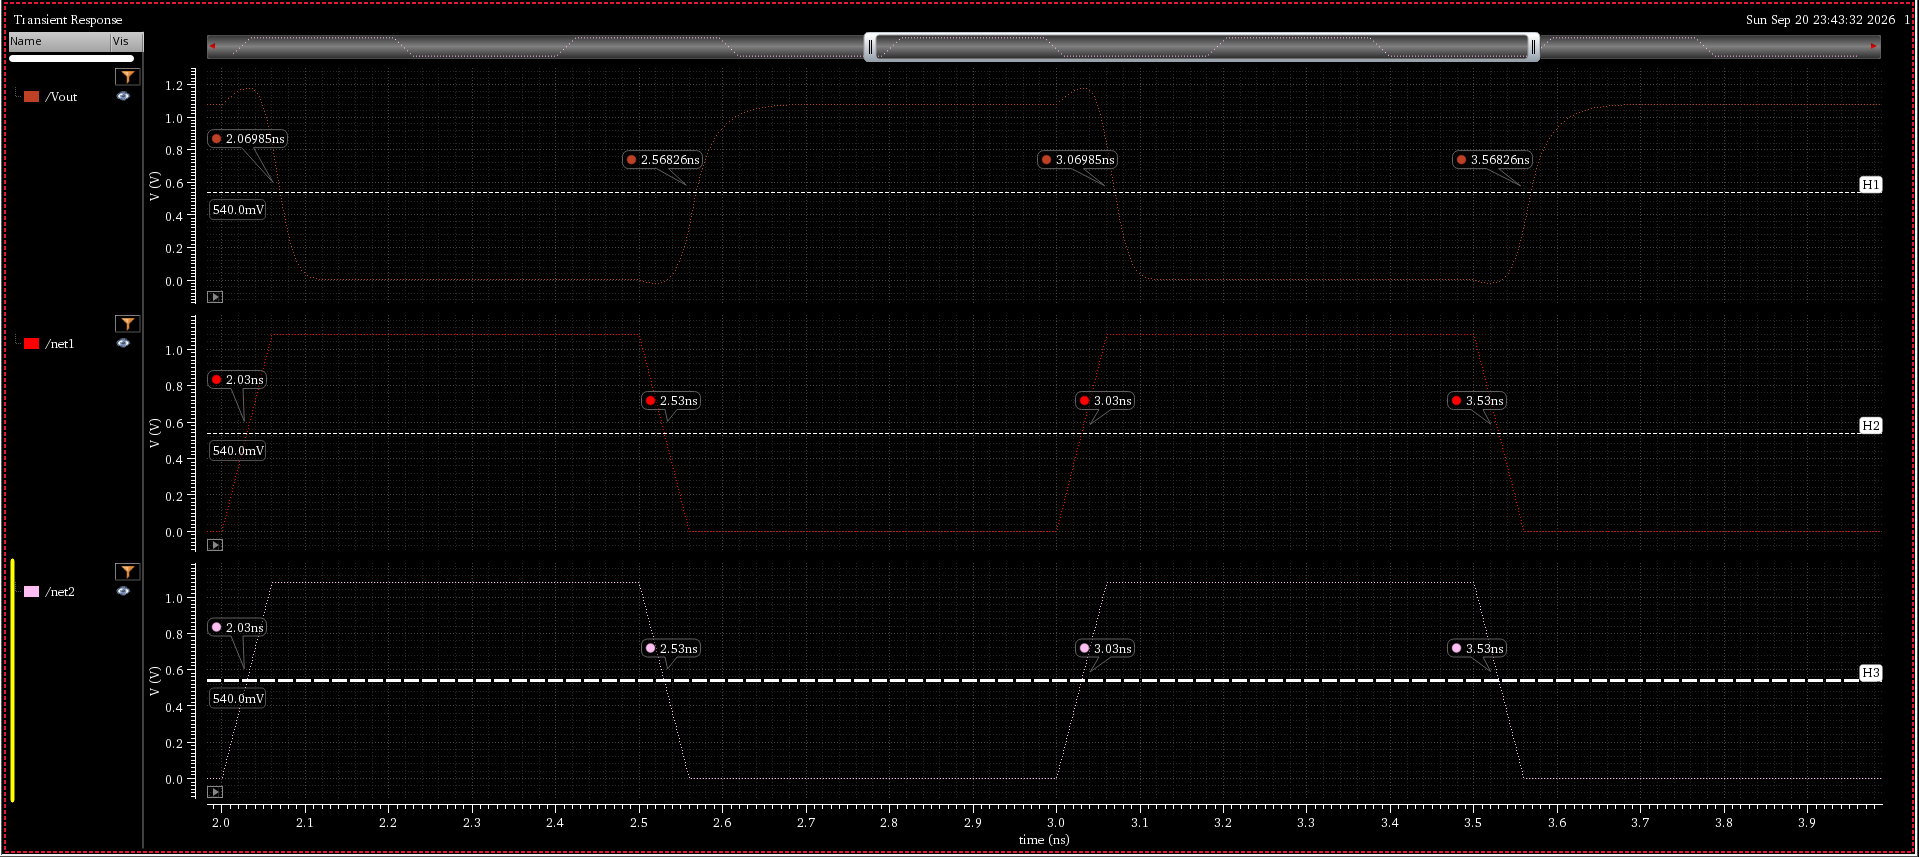
\includegraphics[width=\linewidth]{imagens/NOR_tphl_tplh_SLOW.PNG}
    \caption{Medição de $t_{pHL}$ e $t_{pLH}$ da NOR no corner SLOW, utilizando o nível de $540\,\mathrm{mV}$, correspondente a $50\%$ de $V_{DD}$.}
    \label{fig:nor-slow-atrasos}
\end{figure}

No corner FAST, a saída cruza $660\,\mathrm{mV}$ em $2{,}060299\,\mathrm{ns}$ durante a descida e em $2{,}560130\,\mathrm{ns}$ durante a subida. Subtraindo os instantes correspondentes das entradas, obtêm-se
\begin{align}
    t_{pHL,\mathrm{FAST}} &= (2{,}060299-2{,}030000)\,\mathrm{ns}
                            = 30{,}299\,\mathrm{ps}, \\
    t_{pLH,\mathrm{FAST}} &= (2{,}560130-2{,}530000)\,\mathrm{ns}
                            = 30{,}130\,\mathrm{ps}.
\end{align}

\begin{figure}[!htbp]
    \centering
    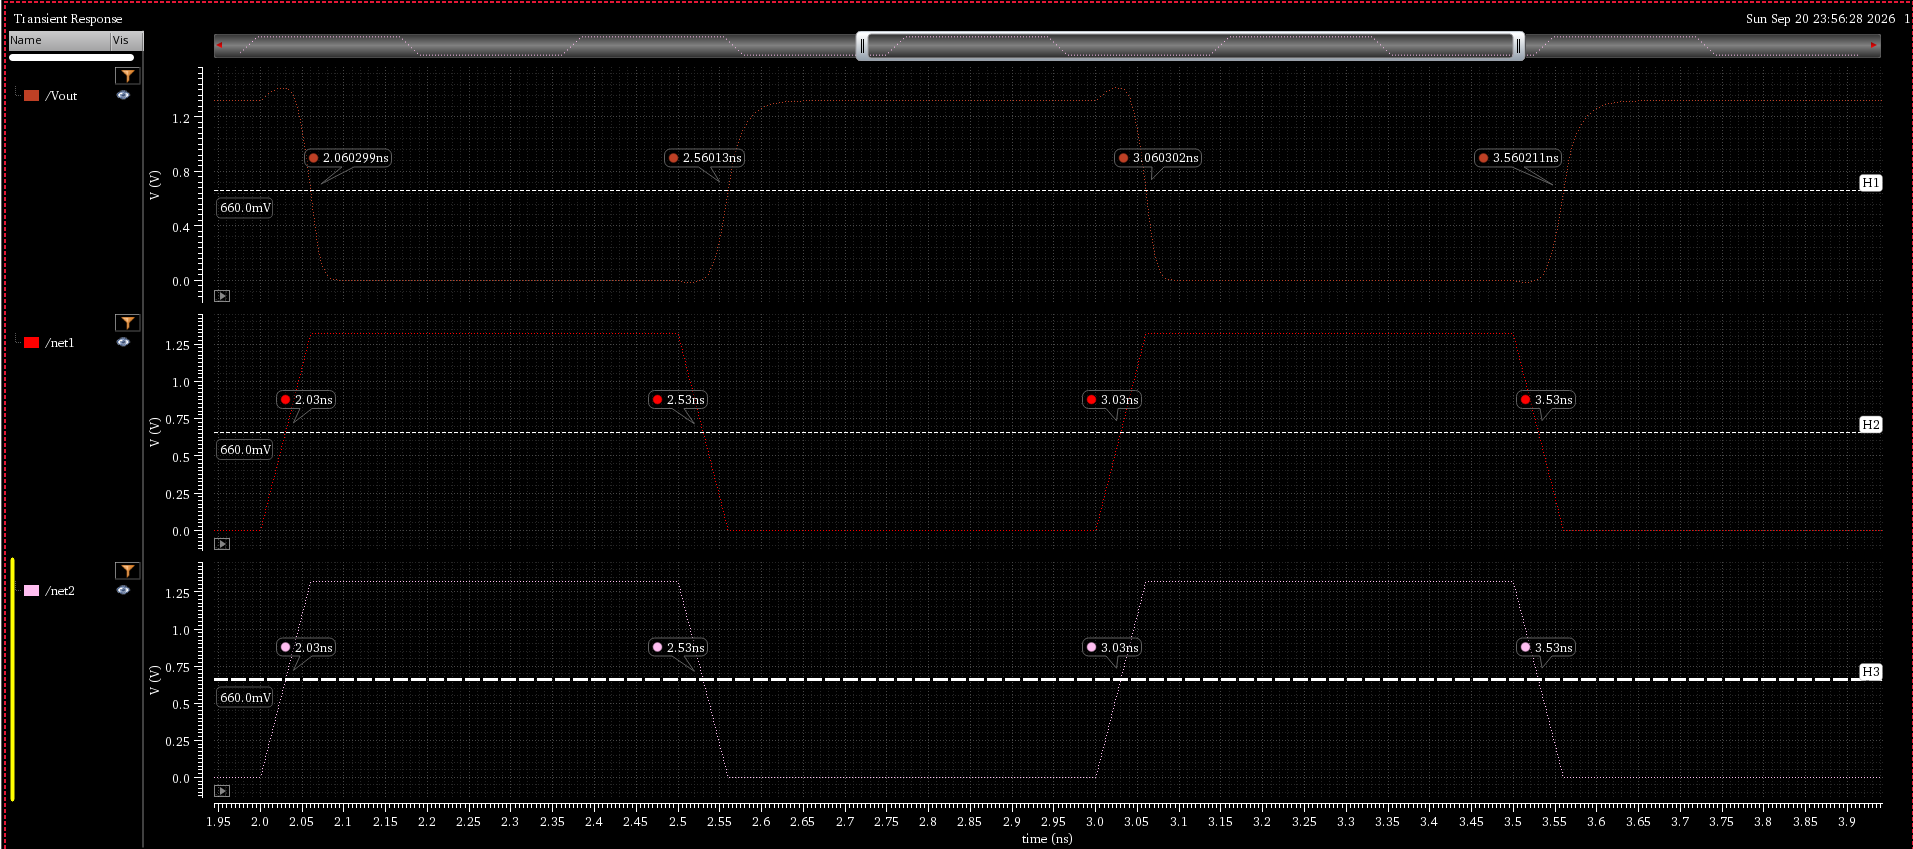
\includegraphics[width=\linewidth]{imagens/NOR_tphl_tplh_FAST.PNG}
    \caption{Medição de $t_{pHL}$ e $t_{pLH}$ da NOR no corner FAST, utilizando o nível de $660\,\mathrm{mV}$, correspondente a $50\%$ de $V_{DD}$.}
    \label{fig:nor-fast-atrasos}
\end{figure}

Os atrasos médios de propagação são $t_{p,\mathrm{SLOW}}=39{,}06\,\mathrm{ps}$ e $t_{p,\mathrm{FAST}}=30{,}21\,\mathrm{ps}$. Mesmo nos corners extremos, $t_{pLH}$ e $t_{pHL}$ permanecem próximos, indicando que o dimensionamento adotado mantém um bom equilíbrio no cruzamento por $50\%$ de $V_{DD}$.

\subsubsection{Tempos de subida e de descida}

Os tempos de transição foram medidos entre $10\%$ e $90\%$ da excursão da saída. Conforme a Figura~\ref{fig:nor-slow-transicoes}, o corner SLOW apresenta $t_r=60{,}17\,\mathrm{ps}$ e $t_f=35{,}63\,\mathrm{ps}$. No corner FAST, mostrado na Figura~\ref{fig:nor-fast-transicoes}, foram obtidos $t_r=43{,}41\,\mathrm{ps}$ e $t_f=25{,}62\,\mathrm{ps}$.

\begin{figure}[!htbp]
    \centering
    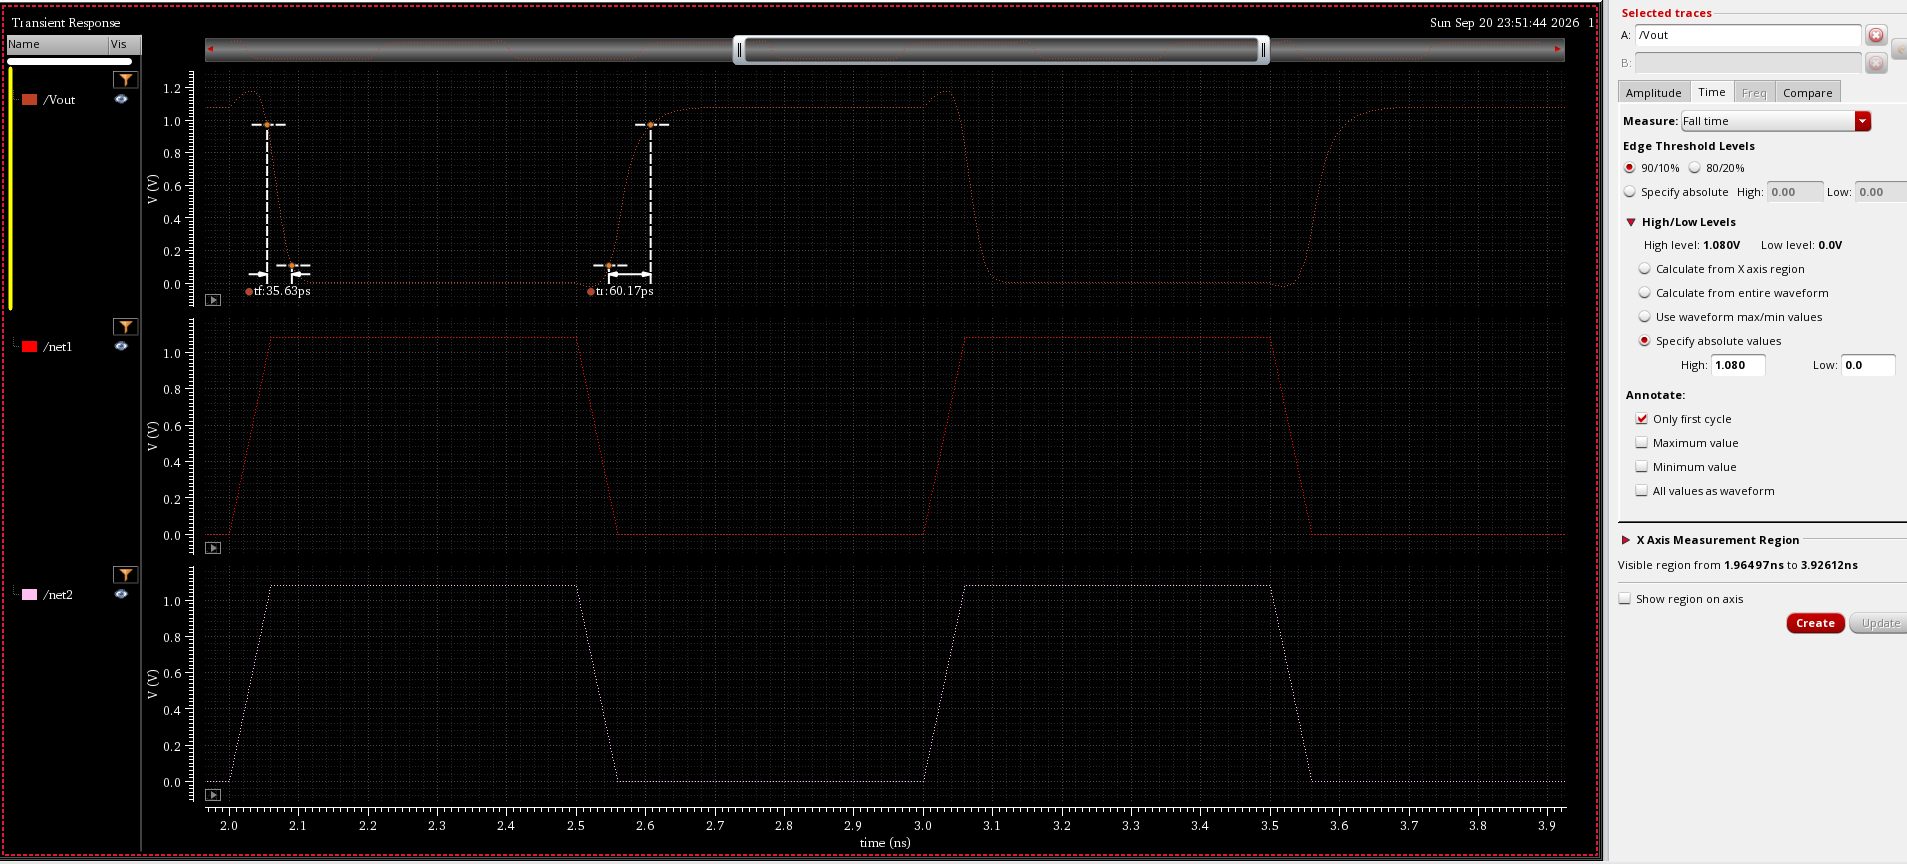
\includegraphics[width=\linewidth]{imagens/NOR_tf_tr_SLOW.PNG}
    \caption{Tempos de subida e de descida da NOR no corner SLOW, medidos pelo critério de $10\%$--$90\%$: $t_r=60{,}17\,\mathrm{ps}$ e $t_f=35{,}63\,\mathrm{ps}$.}
    \label{fig:nor-slow-transicoes}
\end{figure}

\begin{figure}[!htbp]
    \centering
    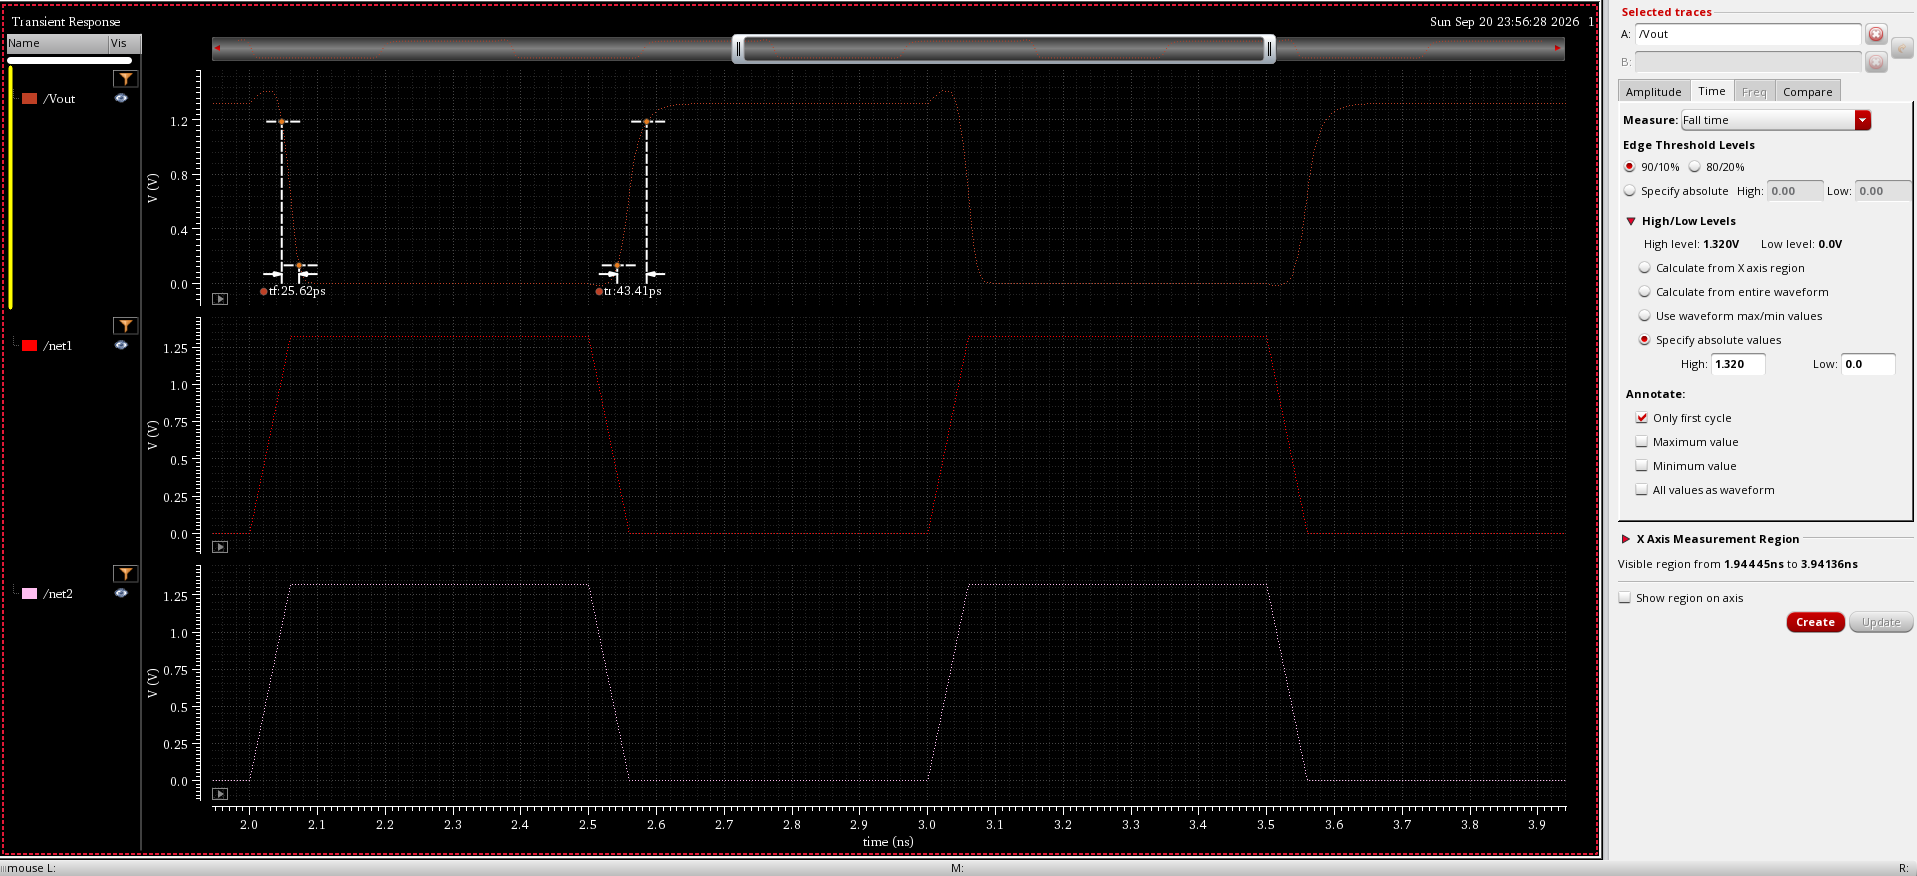
\includegraphics[width=\linewidth]{imagens/NOR_tf_tr_FAST.PNG}
    \caption{Tempos de subida e de descida da NOR no corner FAST, medidos pelo critério de $10\%$--$90\%$: $t_r=43{,}41\,\mathrm{ps}$ e $t_f=25{,}62\,\mathrm{ps}$.}
    \label{fig:nor-fast-transicoes}
\end{figure}

\FloatBarrier

\subsubsection{Comparação entre as condições de simulação}

A Tabela~\ref{tab:nor-corners} compara os resultados dos corners típico, SLOW e FAST. Os valores típicos foram obtidos anteriormente com $V_{DD}=1{,}2\,\mathrm{V}$ e temperatura de $27\,^{\circ}\mathrm{C}$.

\begin{table}[!htbp]
    \centering
    \caption{Comparação dos tempos da porta NOR nas condições típica, SLOW e FAST.}
    \label{tab:nor-corners}
    \begin{tabular}{lcccccc}
        \hline
        Condição & $V_{DD}$ ($\mathrm{V}$) & $T$ ($^{\circ}\mathrm{C}$) & $t_{pLH}$ ($\mathrm{ps}$) & $t_{pHL}$ ($\mathrm{ps}$) & $t_r$ ($\mathrm{ps}$) & $t_f$ ($\mathrm{ps}$) \\
        \hline
        Típica & $1{,}20$ & $27$  & $33{,}33$ & $33{,}41$ & $47{,}93$ & $28{,}08$ \\
        SLOW   & $1{,}08$ & $125$ & $38{,}26$ & $39{,}85$ & $60{,}17$ & $35{,}63$ \\
        FAST   & $1{,}32$ & $0$   & $30{,}13$ & $30{,}30$ & $43{,}41$ & $25{,}62$ \\
        \hline
    \end{tabular}
\end{table}

Em relação à condição típica, o corner SLOW aumenta $t_{pLH}$ em aproximadamente $14{,}8\%$ e $t_{pHL}$ em $19{,}3\%$. O atraso médio passa de $33{,}37\,\mathrm{ps}$ para $39{,}06\,\mathrm{ps}$, crescimento de cerca de $17{,}0\%$. Os tempos de subida e de descida aumentam $25{,}5\%$ e $26{,}9\%$, respectivamente. O aumento de todos os tempos é compatível com a condição WCS: a redução de $V_{DD}$ diminui a sobre-excitação dos transistores, enquanto a temperatura elevada reduz a mobilidade dos portadores. Embora os atrasos medidos a $50\%$ permaneçam equilibrados, a borda de subida continua consideravelmente mais lenta que a borda de descida, devido ao carregamento da saída através dos dois PMOS em série.

No corner FAST, $t_{pLH}$ e $t_{pHL}$ diminuem aproximadamente $9{,}6\%$ e $9{,}3\%$, respectivamente. O atraso médio é reduzido para $30{,}21\,\mathrm{ps}$, cerca de $9{,}5\%$ abaixo do valor típico. Os tempos $t_r$ e $t_f$ diminuem $9{,}4\%$ e $8{,}8\%$. A maior tensão de alimentação e a menor temperatura aumentam a capacidade de condução dos transistores, produzindo transições mais rápidas. Como na análise da NAND, a redução dos tempos ocorre ao custo de maior energia dinâmica de comutação, aproximadamente proporcional a $C_LV_{DD}^{2}$.

Portanto, os resultados da NOR seguem a tendência esperada: o corner SLOW representa o pior caso de velocidade e o corner FAST fornece os menores tempos. A variação do atraso médio é aproximadamente simétrica em torno do corner típico, enquanto a assimetria entre $t_r$ e $t_f$ permanece em todas as condições, refletindo a diferença topológica entre a rede PMOS em série e a rede NMOS em paralelo.

\section{Desenho do layout da porta NOR}

O layout da porta NOR foi desenvolvido seguindo as mesmas convenções gerais adotadas para a NAND: rede PMOS próxima a $V_{DD}$, rede NMOS próxima a $V_{SS}$, segmentos predominantemente verticais em Metal~1 e segmentos horizontais em Metal~2. Para evitar redundância, esta seção enfatiza as particularidades da NOR e os resultados específicos de sua verificação física.

\subsection{Estratégia de desenho e roteamento}

A Figura~\ref{fig:nor-layout} apresenta o layout completo. A principal diferença em relação à NAND é a área ocupada pela rede PMOS. Como cada PMOS da NOR possui $W_p=8{,}5\,\mu\mathrm{m}$ e os dois dispositivos formam o caminho de carga em série, essa rede domina a altura da célula. Os NMOS, com $W_n=1\,\mu\mathrm{m}$ e conexão em paralelo, ocupam uma região menor próxima à barra de $V_{SS}$.

\begin{figure}[!htbp]
    \centering
    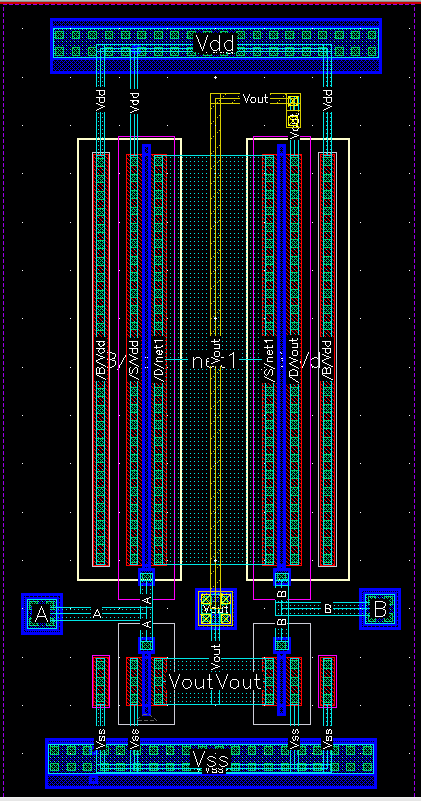
\includegraphics[width=0.52\linewidth]{imagens/NOR_layout.PNG}
    \caption{Layout da porta NOR, com a extensa rede PMOS em série na região superior e a rede NMOS em paralelo próxima à barra de $V_{SS}$.}
    \label{fig:nor-layout}
\end{figure}

As barras de alimentação foram mantidas nas extremidades superior e inferior. As entradas $A$ e $B$ foram posicionadas nas laterais e roteadas até as portas dos dispositivos. O nó de saída reúne o terminal inferior da associação PMOS e os drenos dos NMOS em paralelo. %Assim como no layout da NAND, a separação direcional entre Metal~1 e Metal~2 foi utilizada para reduzir cruzamentos: conexões verticais percorrem majoritariamente Metal~1, enquanto os trechos horizontais utilizam Metal~2 e vias de transição.

Os dispositivos foram posicionados próximos para limitar o comprimento das interconexões, mas preservando espaço para contatos, vias e alinhamento entre as redes. No caso da NOR, esse espaçamento foi especialmente importante por causa da grande largura dos PMOS e da necessidade de conduzir separadamente as duas entradas até a rede superior sem colisão com a saída.

\subsection{Definição dos pinos}

A configuração mostrada na Figura~\ref{fig:nor-pin-placement} apresenta os terminais da célula no \textit{Pin Planner}, mostrando as camadas onde desenhamos cada pino. %Antes da verificação final, os pinos e suas conexões foram revisados para manter no layout os mesmos cinco terminais do esquemático: as entradas $A$ e $B$, a saída $V_{out}$ e as alimentações $V_{DD}$ e $V_{SS}$.

\begin{figure}[!htbp]
    \centering
    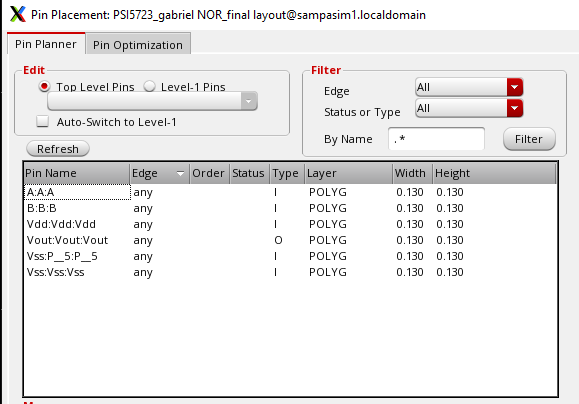
\includegraphics[width=0.78\linewidth]{imagens/NOR_pin_placement.PNG}
    \caption{Configuração dos pinos da porta NOR no \textit{Pin Planner}.}
    \label{fig:nor-pin-placement}
\end{figure}

Os pinos foram associados às formas condutoras correspondentes, com nomes e finalidades consistentes entre o esquemático, o layout e o arquivo de regras. Essa correspondência permitiu o reconhecimento correto das redes durante a comparação LVS.

\subsection{Verificação DRC}

O Calibre nmDRC reportou 274 marcadores distribuídos em 13 das 15 verificações listadas, conforme a Figura~\ref{fig:nor-drc}. A regra selecionada, \texttt{OD.DN.3}, exige densidade mínima de $25\%$ de difusão na área total analisada. As categorias apresentadas são as mesmas observadas na célula NAND e estão relacionadas às verificações globais de densidade e área vazia do arquivo que contém apenas a célula isolada.

\begin{figure}[!htbp]
    \centering
    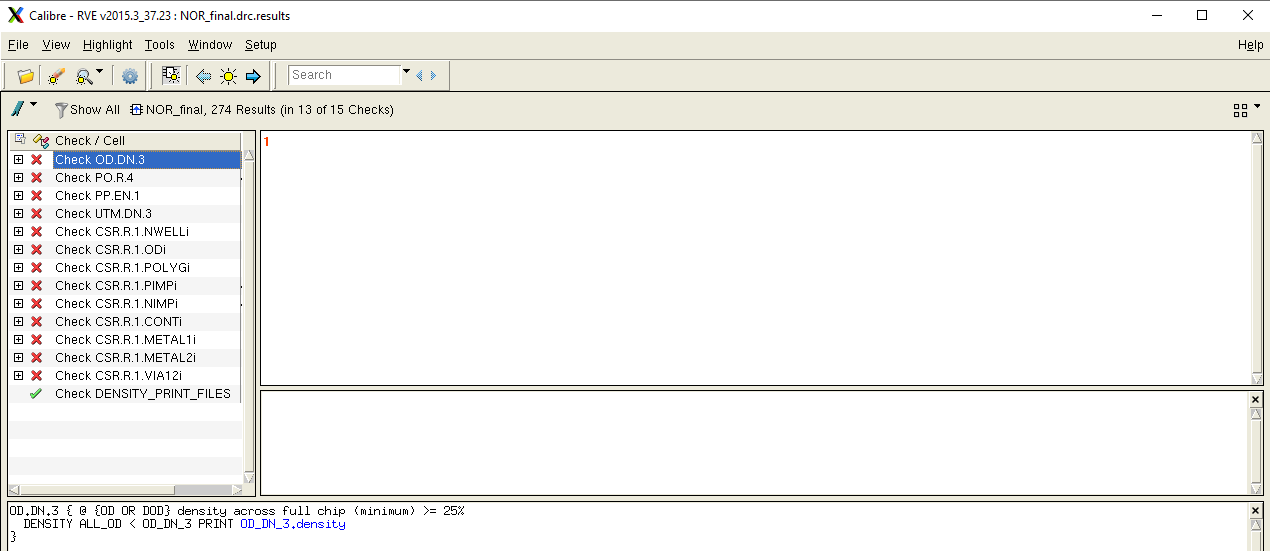
\includegraphics[width=\linewidth]{imagens/NOR_Callibre_nmDRC.PNG}
    \caption{Resultados do Calibre nmDRC para a NOR. A regra selecionada corresponde à densidade mínima de difusão na área total do chip.}
    \label{fig:nor-drc}
\end{figure}

Esses marcadores foram desconsiderados nesta etapa pelo mesmo motivo discutido para a NAND: não há um chip completo, células vizinhas ou preenchimento de densidade ao redor da porta. O número maior de ocorrências em relação à NAND também é compatível com a maior área geométrica da NOR. Ainda assim, o resultado não deve ser apresentado como um DRC limpo. Em uma implementação destinada à fabricação, seria necessário incluir estruturas de preenchimento adequadas e repetir a verificação até a eliminação ou aprovação formal de todos os marcadores.

\subsection{Verificação LVS e extração de parasitas}

A verificação LVS da NOR foi concluída com sucesso. Conforme a Figura~\ref{fig:nor-lvs}, o Calibre apresentou o resultado \textit{CORRECT}, com correspondência de cinco portas, seis redes e quatro transistores entre o layout e o esquemático. Desse modo, a equivalência elétrica da célula foi confirmada antes da extração dos parasitas.

\begin{figure}[!htbp]
    \centering
    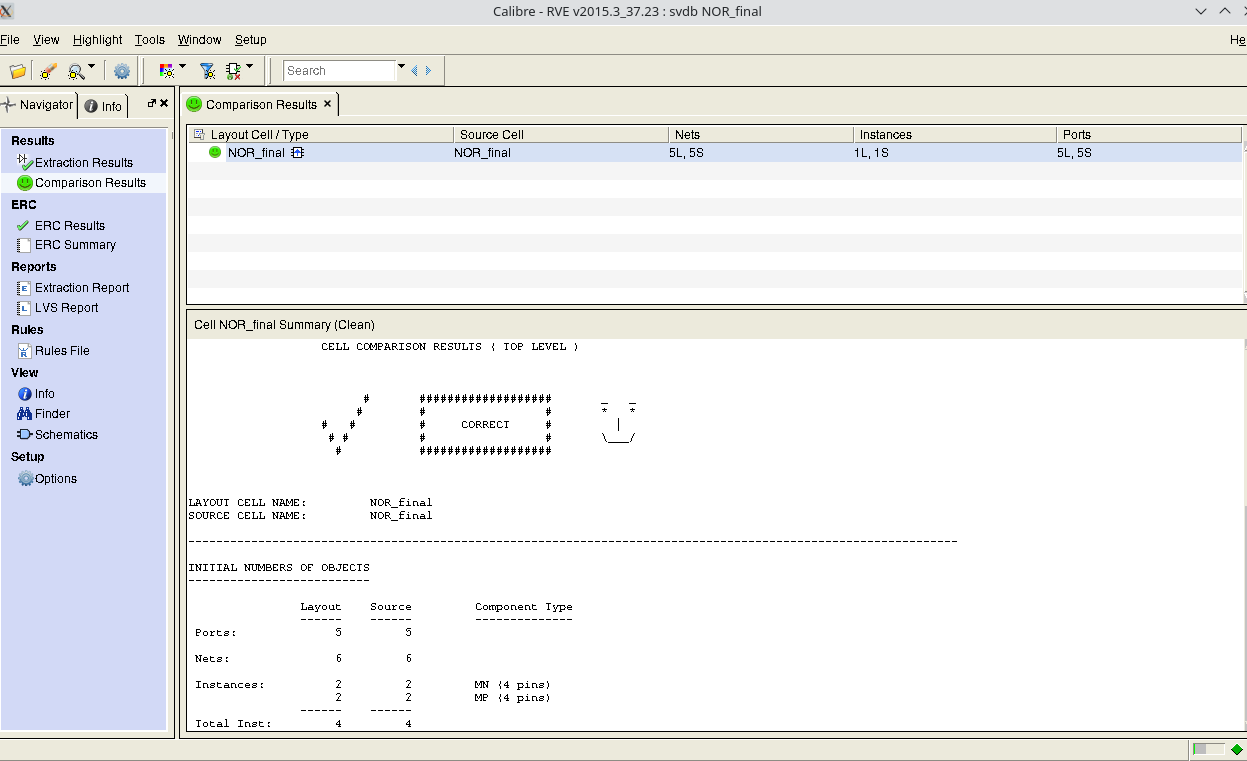
\includegraphics[width=\linewidth]{imagens/LVS_update/NOR_LVS_validated.png}
    \caption{Resultado da verificação LVS da porta NOR no Calibre, com correspondência correta entre layout e esquemático.}
    \label{fig:nor-lvs}
\end{figure}

Após a validação, o Calibre PEX foi empregado para extrair as resistências e capacitâncias parasitas. A Tabela~\ref{tab:nor-parasitas} relaciona as redes do layout às redes do esquemático e apresenta as capacitâncias extraídas.

\begin{table}[!htbp]
    \centering
    \scriptsize
    \caption{Resumo dos parasitas extraídos pelo Calibre PEX para cada rede do layout da NOR.}
    \label{tab:nor-parasitas}
    \resizebox{\linewidth}{!}{%
    \begin{tabular}{llcccc}
        \hline
        Rede no layout & Rede no esquemático & \texttt{R\_Count} & $C_{\mathrm{tot}}$ ($\mathrm{F}$) & $C_C$ ($\mathrm{F}$) & $C_{\mathrm{tot}}+C_C$ ($\mathrm{F}$) \\
        \hline
        \texttt{A}    & \texttt{A}    & $10$ & $5{,}23102\times10^{-16}$ & $2{,}04131\times10^{-16}$ & $7{,}27233\times10^{-16}$ \\
        \texttt{Vss}  & \texttt{VSS}  & $21$ & $1{,}36990\times10^{-15}$ & $2{,}71539\times10^{-16}$ & $1{,}64144\times10^{-15}$ \\
        \texttt{Vout} & \texttt{VOUT} & $23$ & $7{,}24163\times10^{-16}$ & $2{,}13181\times10^{-15}$ & $2{,}85597\times10^{-15}$ \\
        \texttt{B}    & \texttt{B}    & $10$ & $5{,}11269\times10^{-16}$ & $2{,}05629\times10^{-16}$ & $7{,}16898\times10^{-16}$ \\
        \texttt{Vdd}  & \texttt{VDD}  & $12$ & $1{,}20169\times10^{-15}$ & $1{,}06630\times10^{-15}$ & $2{,}26799\times10^{-15}$ \\
        \texttt{6}    & \texttt{NET1} & $5$  & $7{,}81576\times10^{-16}$ & $2{,}10613\times10^{-15}$ & $2{,}88771\times10^{-15}$ \\
        \hline
    \end{tabular}%
    }
\end{table}

Na NOR, as maiores capacitâncias combinadas são observadas no nó interno \texttt{NET1}, com $2{,}88771\,\mathrm{fF}$, e na saída, com $2{,}85597\,\mathrm{fF}$. Em ambos os casos, a capacitância de acoplamento é a contribuição predominante. A rede $V_{DD}$ também apresenta capacitância significativa, igual a $2{,}26799\,\mathrm{fF}$.

As Figuras~\ref{fig:nor-pex-normal}--\ref{fig:nor-pex-fast} apresentam as simulações do circuito extraído nas condições típica, SLOW e FAST.

\begin{figure}[!htbp]
    \centering
    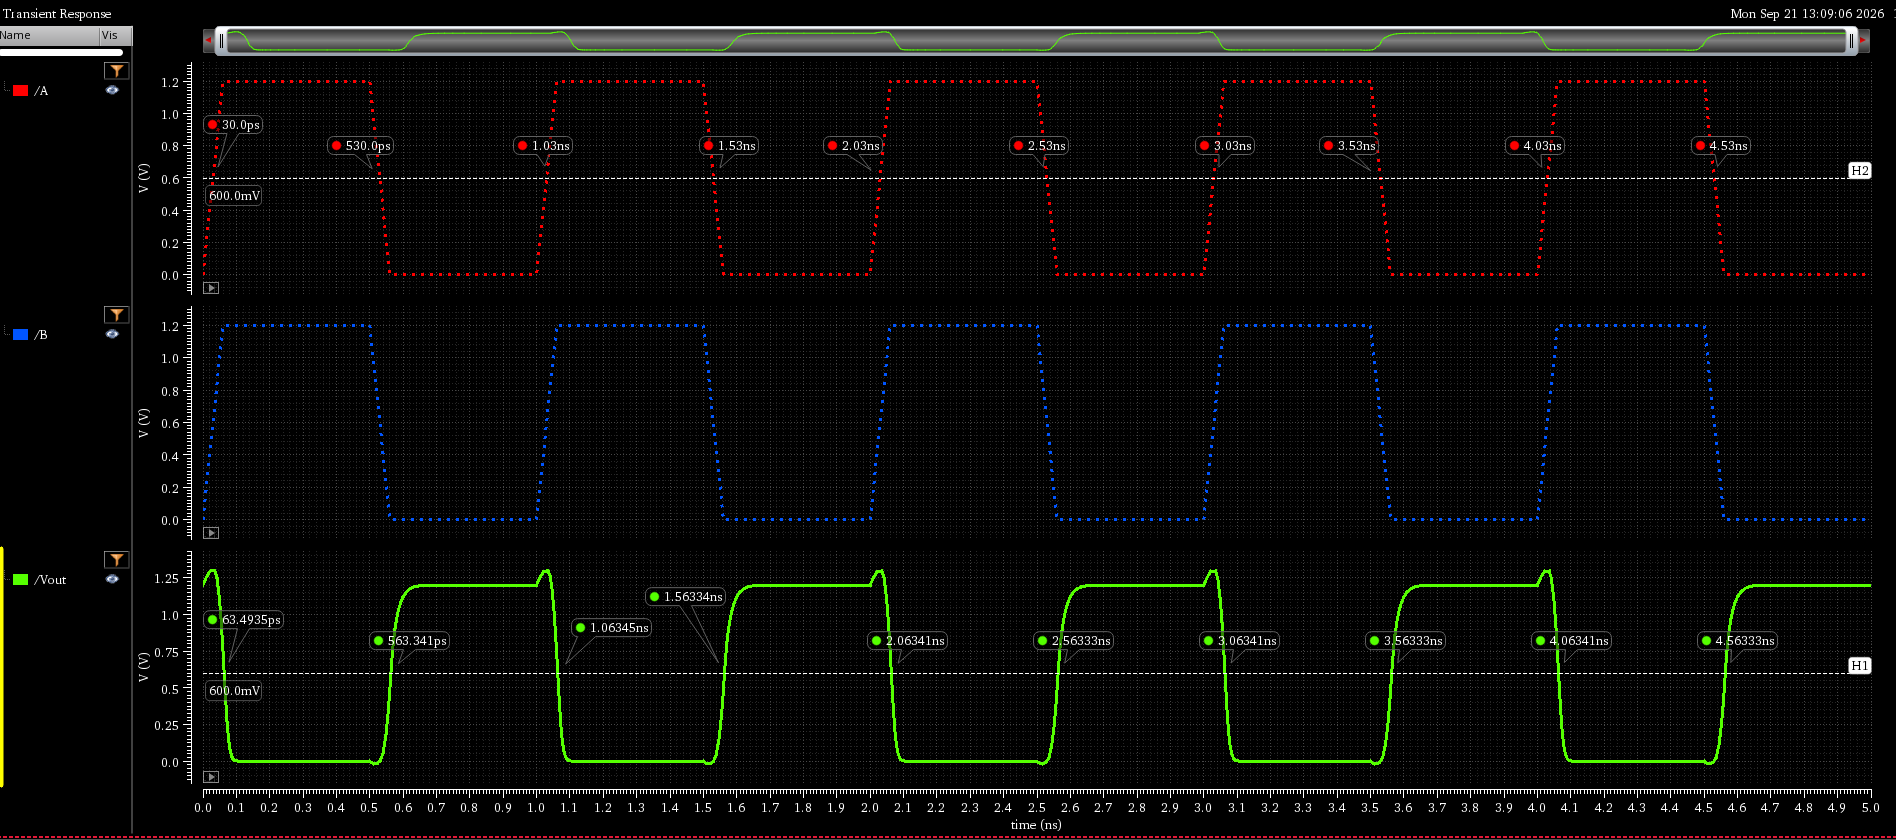
\includegraphics[width=\linewidth]{imagens/LVS_update/NOR_PEX_NORMAL_SIMULATION_2.png}
    \caption{Simulação PEX da NOR na condição típica para a medição dos atrasos de propagação: $t_{pLH}=33{,}34\,\mathrm{ps}$ e $t_{pHL}=33{,}45\,\mathrm{ps}$.}
    \label{fig:nor-pex-normal}
\end{figure}

\FloatBarrier

Utilizando os marcadores da Figura~\ref{fig:nor-pex-normal}, na condição típica, obtêm-se
\begin{align}
    t_{pHL} &= (1{,}06345-1{,}03000)\,\mathrm{ns}
             =33{,}45\,\mathrm{ps}, \\
    t_{pLH} &= (1{,}56334-1{,}53000)\,\mathrm{ns}
             =33{,}34\,\mathrm{ps}, \\
    t_p &= \frac{t_{pLH}+t_{pHL}}{2}
          =33{,}40\,\mathrm{ps}.
\end{align}
Os tempos de transição são extraídos da Figura~\ref{fig:nor-pex-normal-transicoes}, com níveis de $120\,\mathrm{mV}$ e $1{,}08\,\mathrm{V}$.
\begin{figure}[!htbp]
    \centering
    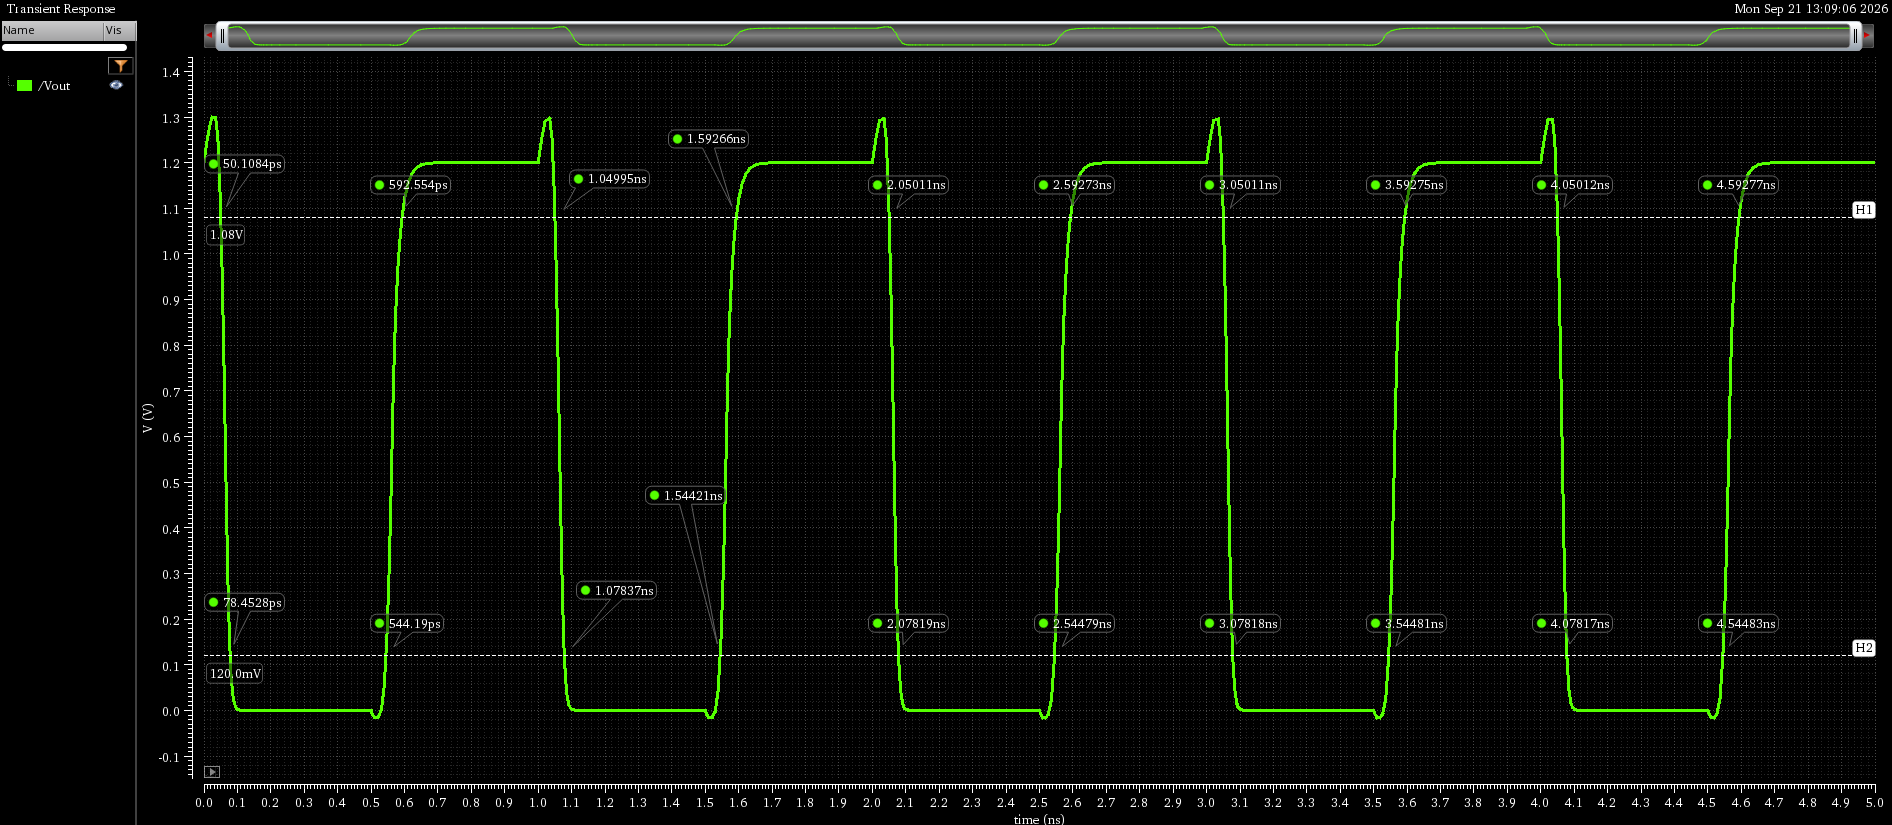
\includegraphics[width=\linewidth]{imagens/LVS_update/NOR_PEX_NORMAL_SIMULATION_TRISE_TFALL_10p90p.png}
    \caption{Medição PEX dos tempos de subida e de descida da NOR na condição típica pelo critério de $10\%$--$90\%$.}
    \label{fig:nor-pex-normal-transicoes}
\end{figure}
\FloatBarrier
\begin{align}
    t_r &= (592{,}554-544{,}190)\,\mathrm{ps}
          =48{,}36\,\mathrm{ps}, \\
    t_f &= (1{,}07837-1{,}04995)\,\mathrm{ns}
          =28{,}42\,\mathrm{ps}.
\end{align}

\begin{figure}[!htbp]
    \centering
    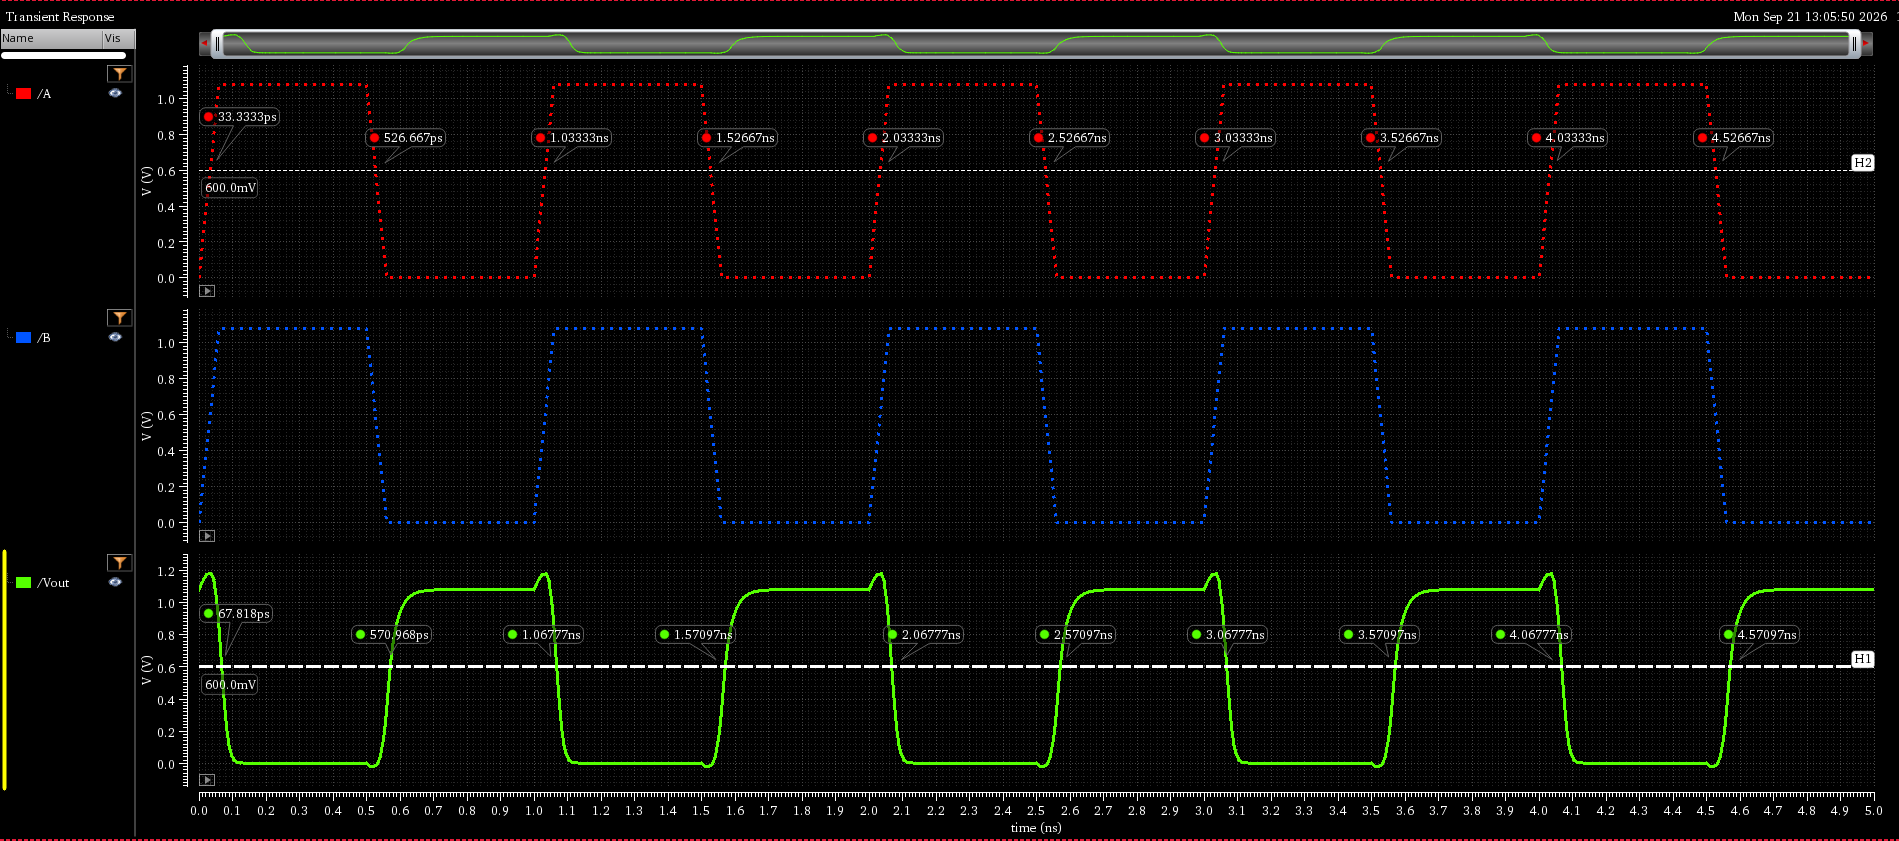
\includegraphics[width=\linewidth]{imagens/LVS_update/NOR_PEX_SLOW_SIMULATION_2.png}
    \caption{Simulação PEX da NOR no corner SLOW para a medição dos atrasos de propagação: $t_{pLH}=44{,}30\,\mathrm{ps}$ e $t_{pHL}=34{,}44\,\mathrm{ps}$.}
    \label{fig:nor-pex-slow}
\end{figure}

\FloatBarrier

No corner SLOW da Figura~\ref{fig:nor-pex-slow}, os atrasos são calculados por
\begin{align}
    t_{pHL} &= (1{,}06777-1{,}03333)\,\mathrm{ns}
             =34{,}44\,\mathrm{ps}, \\
    t_{pLH} &= (1{,}57097-1{,}52667)\,\mathrm{ns}
             =44{,}30\,\mathrm{ps}, \\
    t_p &= \frac{t_{pLH}+t_{pHL}}{2}
          =39{,}37\,\mathrm{ps}.
\end{align}
Para as transições da saída, utilizam-se os marcadores da Figura~\ref{fig:nor-pex-slow-transicoes}, nos níveis de $108\,\mathrm{mV}$ e $972\,\mathrm{mV}$.
\begin{figure}[!htbp]
    \centering
    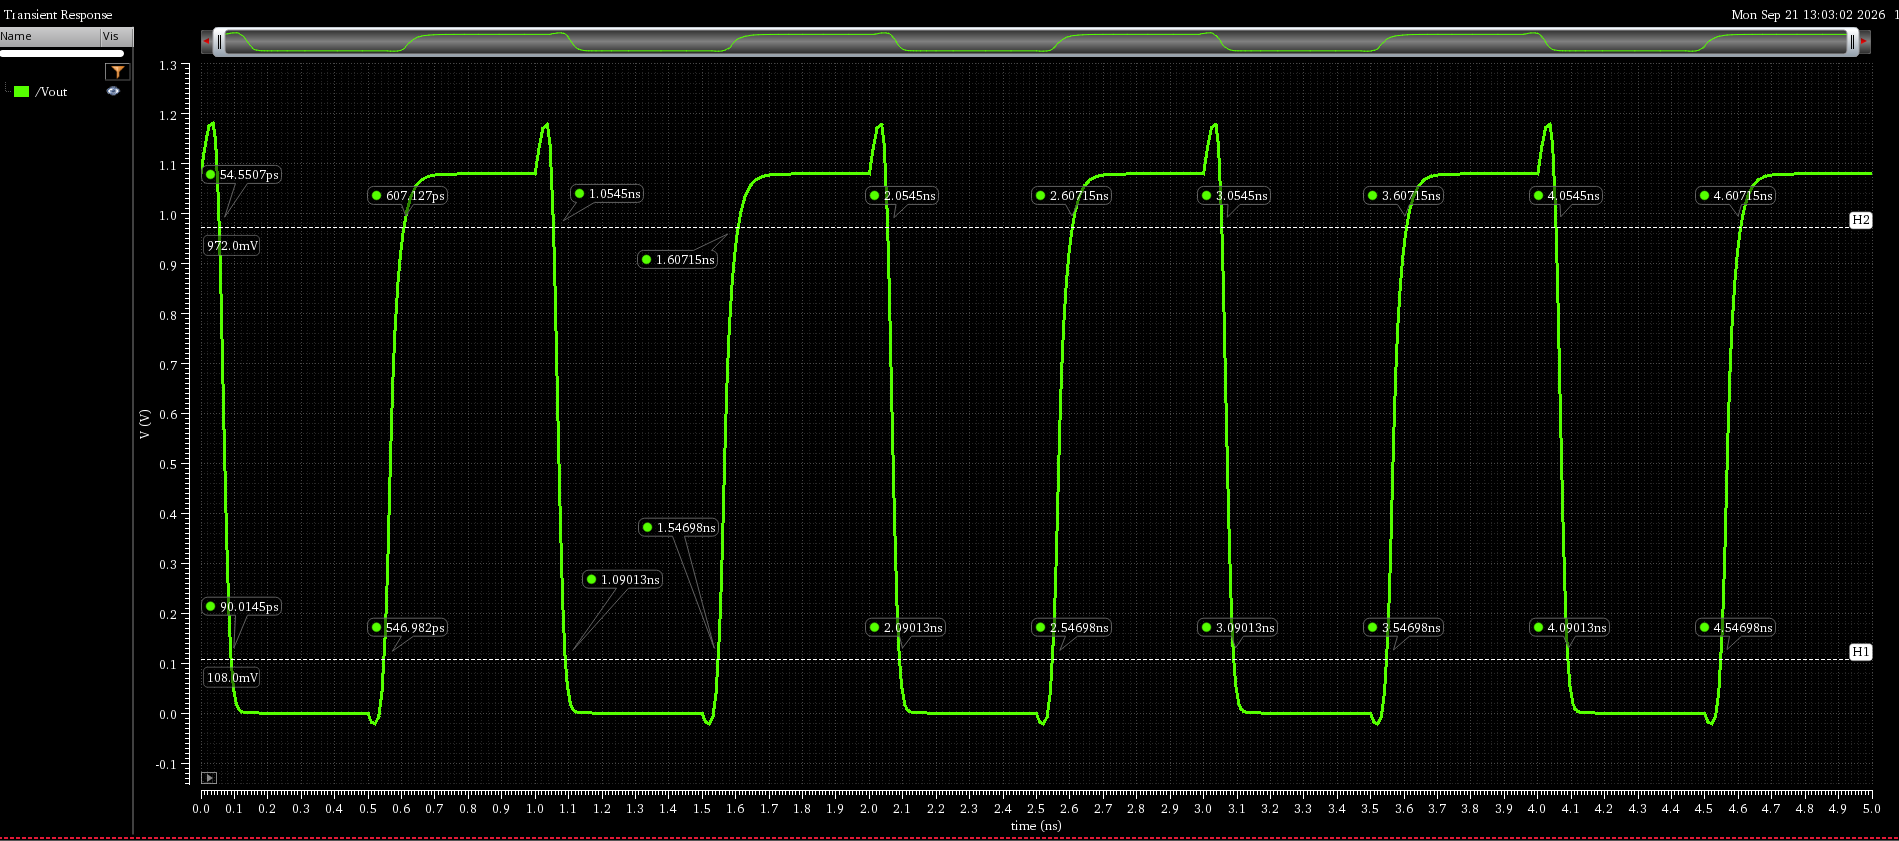
\includegraphics[width=\linewidth]{imagens/LVS_update/NOR_PEX_SLOW_SIMULATION_TRISE_TFALL_10p90p.png}
    \caption{Medição PEX dos tempos de subida e de descida da NOR no corner SLOW pelo critério de $10\%$--$90\%$.}
    \label{fig:nor-pex-slow-transicoes}
\end{figure}
\FloatBarrier
\begin{align}
    t_r &= (607{,}127-546{,}982)\,\mathrm{ps}
          =60{,}15\,\mathrm{ps}, \\
    t_f &= (1{,}09013-1{,}05450)\,\mathrm{ns}
          =35{,}63\,\mathrm{ps}.
\end{align}

\begin{figure}[!htbp]
    \centering
    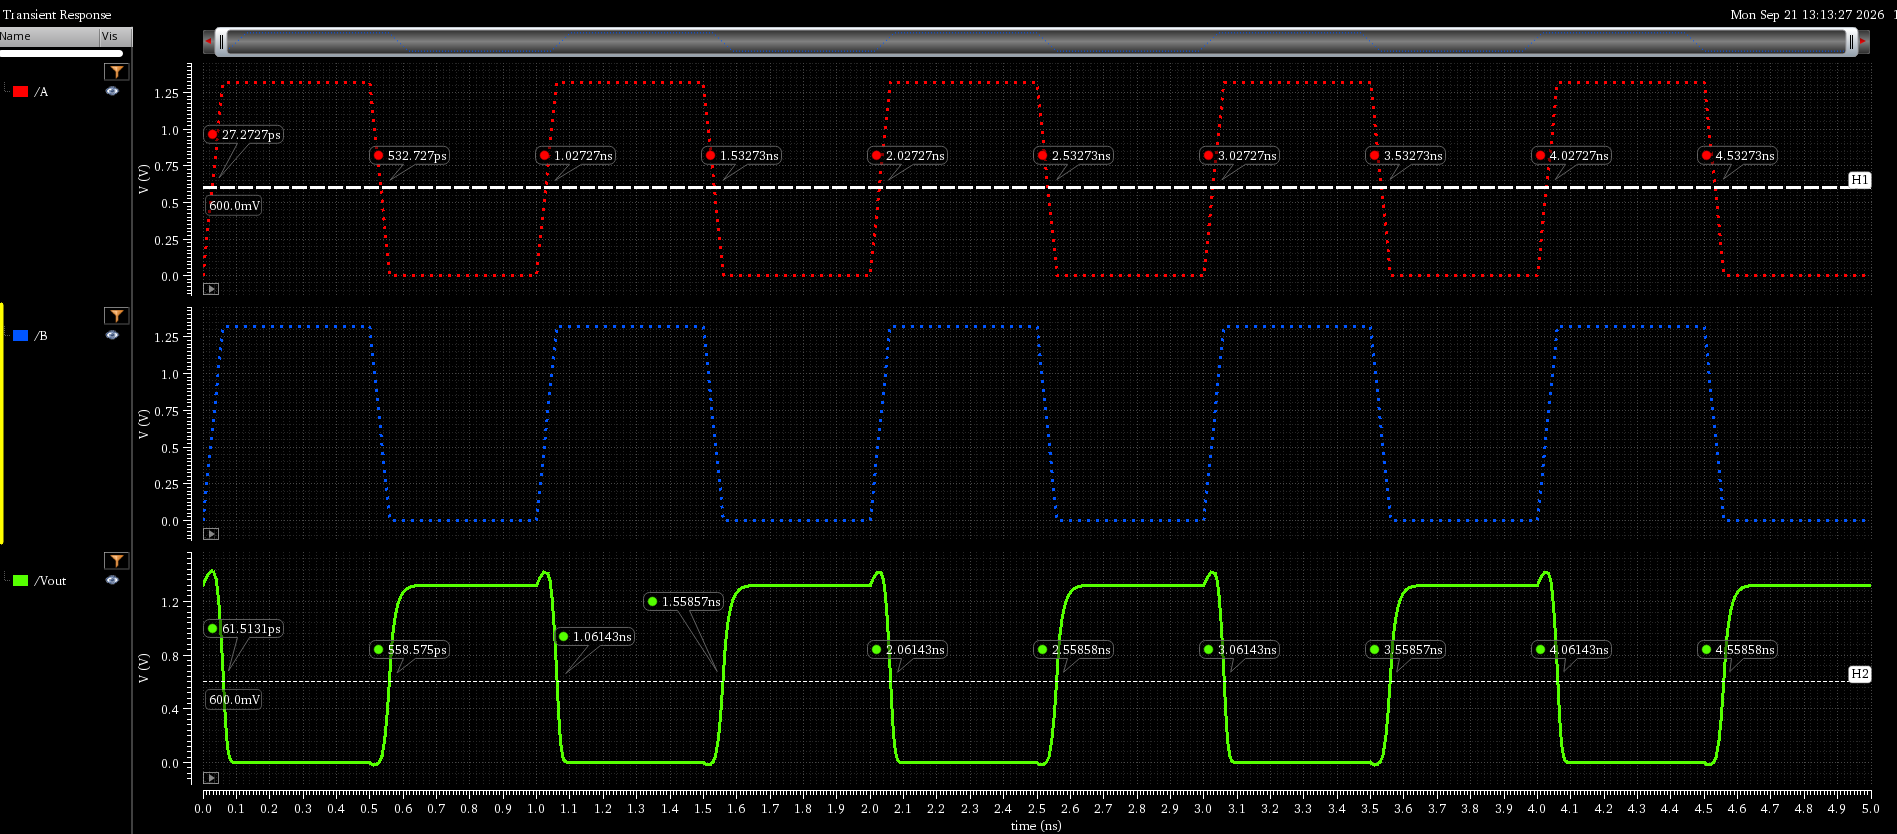
\includegraphics[width=\linewidth]{imagens/LVS_update/NOR_PEX_FAST_SIMULATION_2.png}
    \caption{Simulação PEX da NOR no corner FAST para a medição dos atrasos de propagação: $t_{pLH}=25{,}84\,\mathrm{ps}$ e $t_{pHL}=34{,}16\,\mathrm{ps}$.}
    \label{fig:nor-pex-fast}
\end{figure}

\FloatBarrier

No corner FAST da Figura~\ref{fig:nor-pex-fast}, os marcadores fornecem
\begin{align}
    t_{pHL} &= (1{,}06143-1{,}02727)\,\mathrm{ns}
             =34{,}16\,\mathrm{ps}, \\
    t_{pLH} &= (1{,}55857-1{,}53273)\,\mathrm{ns}
             =25{,}84\,\mathrm{ps}, \\
    t_p &= \frac{t_{pLH}+t_{pHL}}{2}
          =30{,}00\,\mathrm{ps}.
\end{align}
Os tempos de subida e de descida são obtidos da Figura~\ref{fig:nor-pex-fast-transicoes}, nos níveis de $132\,\mathrm{mV}$ e $1{,}188\,\mathrm{V}$.
\begin{figure}[!htbp]
    \centering
    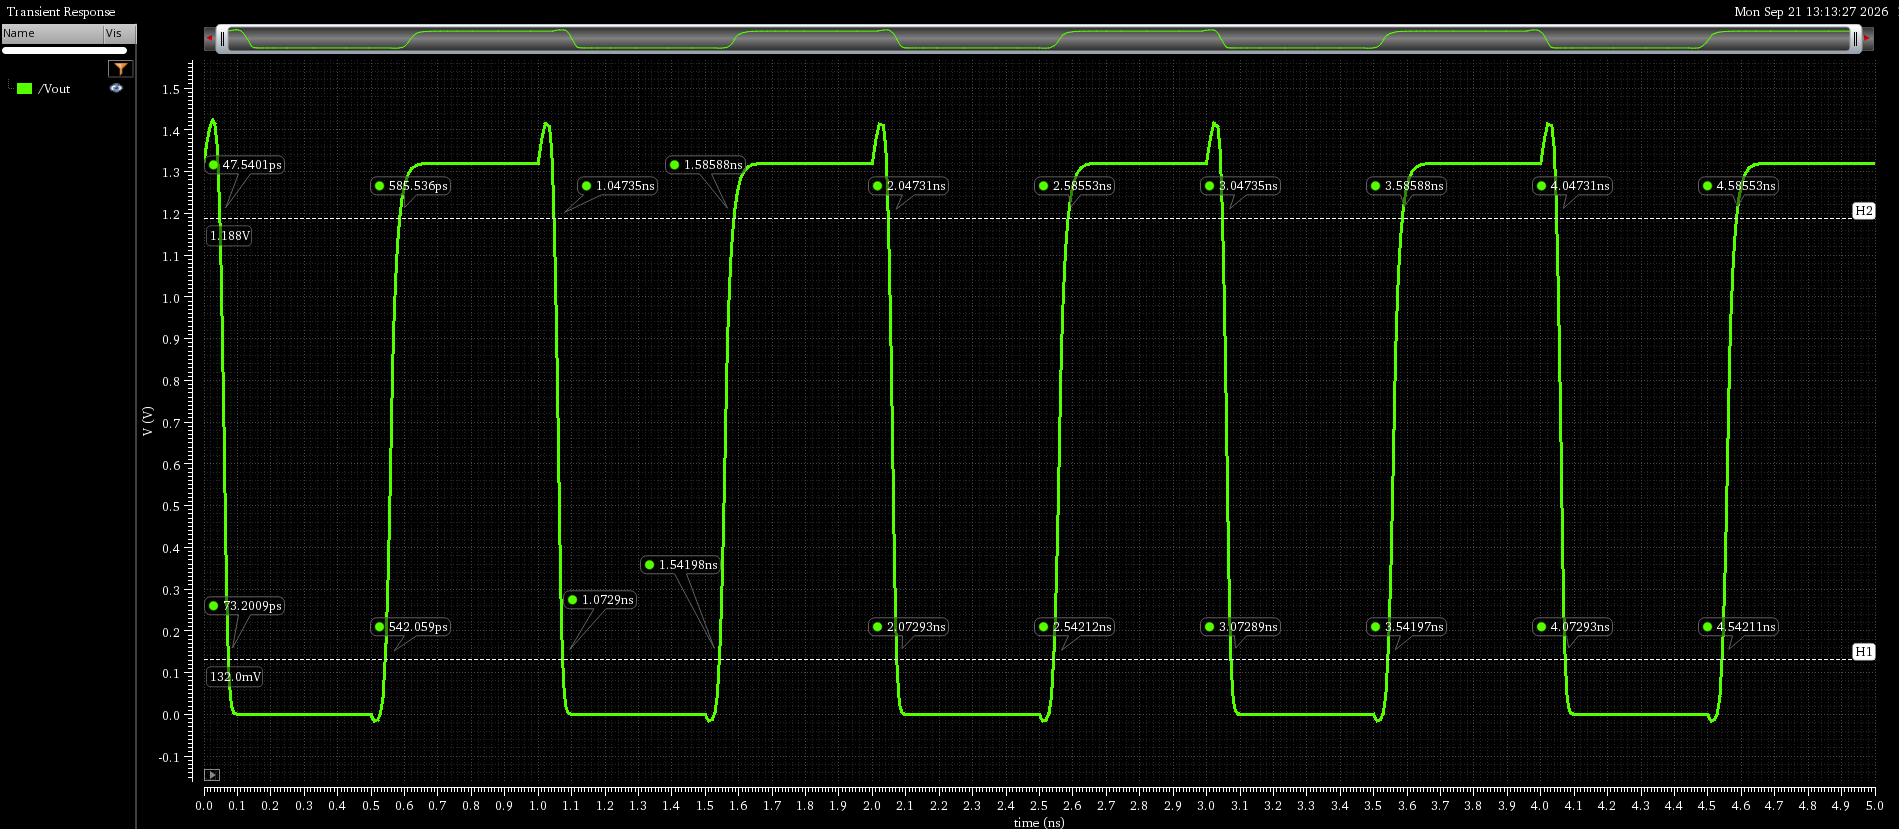
\includegraphics[width=\linewidth]{imagens/LVS_update/NOR_PEX_FAST_SIMULATION_TRISE_TFALL_10p90p.png}
    \caption{Medição PEX dos tempos de subida e de descida da NOR no corner FAST pelo critério de $10\%$--$90\%$.}
    \label{fig:nor-pex-fast-transicoes}
\end{figure}
\FloatBarrier
\begin{align}
    t_r &= (585{,}536-542{,}059)\,\mathrm{ps}
          =43{,}48\,\mathrm{ps}, \\
    t_f &= (1{,}07290-1{,}04730)\,\mathrm{ns}
          =25{,}60\,\mathrm{ps}.
\end{align}

\FloatBarrier

Os resultados calculados para as três condições são comparados aos valores de esquemático na Tabela~\ref{tab:nor-esquematico-pex}.

Assim como na NAND, os atrasos médios e os tempos de transição da NOR extraída permanecem próximos dos valores de esquemático. Os valores de $t_r$ e $t_f$ foram calculados somente a partir das capturas específicas de $10\%$--$90\%$. As capturas de atraso dos três corners utilizam marcadores em $600\,\mathrm{mV}$; por isso, as comparações individuais de $t_{pLH}$ e $t_{pHL}$ nos corners SLOW e FAST devem considerar que as medições anteriores de esquemático utilizaram $50\%$ das respectivas tensões de alimentação.

As colunas $\Delta t_p$ da Tabela~\ref{tab:nor-esquematico-pex} utilizam a mesma definição adotada para a NAND: diferença absoluta e variação percentual do atraso médio PEX em relação ao esquemático no mesmo corner.

\begin{table}[!htbp]
    \centering
    \small
    \caption{Comparação entre as simulações de esquemático e PEX da porta NOR.}
    \label{tab:nor-esquematico-pex}
    \resizebox{\linewidth}{!}{%
    \begin{tabular}{llccccccc}
        \hline
        Condição & Modelo & $t_{pLH}$ ($\mathrm{ps}$) & $t_{pHL}$ ($\mathrm{ps}$) & $t_p$ ($\mathrm{ps}$) & $t_r$ ($\mathrm{ps}$) & $t_f$ ($\mathrm{ps}$) & $\Delta t_p$ ($\mathrm{ps}$) & $\Delta t_p$ ($\%$) \\
        \hline
        Típica & Esquemático & $33{,}33$ & $33{,}41$ & $33{,}37$ & $47{,}93$ & $28{,}08$ & -- & -- \\
        Típica & PEX         & $33{,}34$ & $33{,}45$ & $33{,}40$ & $48{,}36$ & $28{,}42$ & $+0{,}03$ & $+0{,}09$ \\
        SLOW   & Esquemático & $38{,}26$ & $39{,}85$ & $39{,}06$ & $60{,}17$ & $35{,}63$ & -- & -- \\
        SLOW   & PEX         & $44{,}30$ & $34{,}44$ & $39{,}37$ & $60{,}15$ & $35{,}63$ & $+0{,}31$ & $+0{,}79$ \\
        FAST   & Esquemático & $30{,}13$ & $30{,}30$ & $30{,}21$ & $43{,}41$ & $25{,}62$ & -- & -- \\
        FAST   & PEX         & $25{,}84$ & $34{,}16$ & $30{,}00$ & $43{,}48$ & $25{,}60$ & $-0{,}21$ & $-0{,}70$ \\
        \hline
    \end{tabular}%
    }
\end{table}

Conforme obervado na Tabela ~\ref{tab:nor-esquematico-pex}, os parasitas do layout introduziram uma alterção absoluta máxima de 0,79\% apenas.

\end{document}